\documentclass[12pt,a4paper,oneside]{memoir}

% ===============================
% 1. PACKAGES
% ===============================
\usepackage{times}
\usepackage[T1]{fontenc}
\usepackage{xcolor}
\usepackage{graphicx}
\usepackage{amsmath,amssymb}
\usepackage{booktabs}
\usepackage{hyperref}
\usepackage{caption}
\usepackage[backend=biber,style=ieee]{biblatex}
\usepackage{siunitx}
\usepackage{array}
\usepackage{longtable}
\usepackage{placeins}
\usepackage{pdflscape}
\usepackage{lipsum}        % dummy text
\usepackage[linesnumbered,ruled,vlined]{algorithm2e}
\usepackage{float}
%
\usepackage{listings}
% --- Custom Colors for Python Beautification ---
\definecolor{codegreen}{rgb}{0,0.6,0}
\definecolor{codegray}{rgb}{0.5,0.5,0.5}
\definecolor{codepurple}{rgb}{0.58,0,0.82}
\definecolor{backcolour}{rgb}{0.96,0.96,0.97}
\definecolor{codeblue}{rgb}{0.1,0.2,0.8}
% --- Global Listings Style ---
\lstset{
	backgroundcolor=\color{backcolour},   
	commentstyle=\color{codegreen},
	keywordstyle=\color{codeblue}\bfseries,
	numberstyle=\tiny\color{codegray},
	stringstyle=\color{codepurple},
	basicstyle=\ttfamily\scriptsize,
	breakatwhitespace=false,         
	breaklines=true,                 
	captionpos=b,                    
	keepspaces=true,                 
	numbers=left,                    
	numbersep=8pt,                  
	showspaces=false,                
	showstringspaces=false,
	showtabs=false,                  
	tabsize=1,
	frame=single,
	rulecolor=\color{codegray!30},
	language=Python
}

% ===============================
% 2. BIBLIOGRAPHY SETUP
% ===============================
\addbibresource{References.bib}

% ===============================
% 3. COLORS & SPACING
% ===============================
\definecolor{deepred}{RGB}{152,50,34}
\newcommand{\earlierrevision}[1]{\textcolor{blue}{#1}}
\newcommand{\newrevision}[1]{\textcolor{green!45!black}{#1}}
\linespread{1.25}
\setlength{\parindent}{0pt}
\setlength{\parskip}{6pt}
\hyphenpenalty=10000
\exhyphenpenalty=10000
\emergencystretch=3em

% ===============================
% 4. PAGE LAYOUT
% ===============================
\setlrmarginsandblock{1.1in}{1.1in}{*}
\setulmarginsandblock{1in}{1in}{*}
\checkandfixthelayout
\pagestyle{plain}

% ===============================
% 5. NUMBERING & TOC DEPTH
% ===============================
\setsecnumdepth{subsubsection}
\maxsecnumdepth{subsubsection}
\settocdepth{subsection}
\setcounter{tocdepth}{2}

% ===============================
% 6. CHAPTER STYLE (Centered & ALL CAPS)
% ===============================
\makechapterstyle{sdpstyle}{
	\renewcommand{\printchaptername}{}
	\renewcommand{\chapternamenum}{}
	\renewcommand{\printchapternum}{\centering\large\bfseries \thechapter.\space}
	\renewcommand{\chaptitlefont}{\large\bfseries\centering}
	\renewcommand{\afterchapternum}{}
	\renewcommand{\printchaptertitle}[1]{%
		\chaptitlefont\MakeUppercase{##1}%
	}
}
\chapterstyle{sdpstyle}

% ===============================
% 7. HEADING STYLES
% ===============================
\hypersetup{
	colorlinks=false,
	linkcolor=black,
	citecolor=black,
	filecolor=black,
	urlcolor=black,
	linktoc=all,
	pdfborder={0 0 0},
}
\setsecheadstyle{\color{black}\normalsize\bfseries\scshape}
\setsubsecheadstyle{\color{black}\normalsize\bfseries\scshape}
\setsubsubsecheadstyle{\color{black}\bfseries\normalshape}
\renewcommand{\thesubsubsection}{\textcolor{black}{\thesubsection.\arabic{subsubsection}}}

% --- Paragraph heading style (memoir native) ---
\setparaheadstyle{\bfseries}
\setafterparaskip{1.5ex plus .4ex minus .2ex}
\setbeforeparaskip{3.25ex plus 1ex minus .2ex}

% ===============================
% 8. TOC STYLING
% ===============================
\renewcommand{\printtoctitle}[1]{\centering\large\bfseries \MakeUppercase{#1}}
\renewcommand{\cftchapterfont}{\scshape\bfseries\color{black}}
\renewcommand{\cftchapterpagefont}{\color{black}}
\renewcommand{\cftsectionfont}{\scshape\color{black}}
\renewcommand{\cftsectionpagefont}{\color{black}}
\renewcommand{\cftsubsectionfont}{\normalshape\color{black}}
\renewcommand{\cftsubsectionpagefont}{\color{black}}

% ===============================
% 9. UNNUMBERED RED HEADING COMMAND
% ===============================
\newcommand{\redheading}[1]{%
	\vspace{6pt}
	{\color{black}\bfseries\normalshape #1}\par
	\noindent
	\vspace{0pt}%
}

% ===============================
% 10. FIGURE & TABLE CAPTIONS
% ===============================
\captionnamefont{\scshape}
\captiontitlefont{\upshape}
\captiondelim{.\ }
\setlength{\belowcaptionskip}{10pt}
\setlength{\abovecaptionskip}{10pt}

% ===============================
% 11. CONTENTS NAME
% ===============================
\renewcommand{\contentsname}{CONTENTS}

% ===============================
% 12. ALGORITHMS (algorithm2e)
% ===============================
\renewcommand{\listalgorithmcfname}{List of Algorithms}

% ===============================
% 13. PAGE NUMBERING & LIST STYLING
% ===============================
\frontmatter
\pagenumbering{roman}

% --- Figure Spacing (Tightened) ---
\renewcommand{\cftfigurename}{Figure~}
\renewcommand{\cftfigureaftersnum}{.}
\setlength{\cftfigurenumwidth}{3.0em} 
\setlength{\cftfigureindent}{0em}    

% --- Table Spacing (Tightened) ---
\renewcommand{\cfttablename}{Table~}
\renewcommand{\cfttableaftersnum}{.}
\setlength{\cfttablenumwidth}{3.0em} 
\setlength{\cfttableindent}{0em}    

% --- Algorithm List Styling ---
\makeatletter
% Force "Algorithm" prefix into the list
\let\oldl@algocf\l@algocf
\renewcommand{\l@algocf}[2]{\oldl@algocf{Algorithm #1}{#2}}

% Direct memoir-style length setting for Algorithms
\AtBeginDocument{
	\newlength{\cftalgocfnumwidth}
	\setlength{\cftalgocfnumwidth}{6em}
	\newlength{\cftalgocfindent}
	\setlength{\cftalgocfindent}{0em}
}
\makeatother

% ===============================
% 14. APPENDIX SETUP 
% ===============================
\makeatletter
\g@addto@macro\appendix{%
	% 1. Force A, B, C numbering
	\renewcommand{\thechapter}{\Alph{chapter}}
	
	% 2. Fix the Header on the actual page
	\renewcommand{\printchapternum}{%
		\centering\large\bfseries APPENDIX \thechapter.\space%
	}
	
	% 3. Override the chapter command
	\def\chapter{\@ifstar{\@schapter}{\@dblarg\@manualappendixchapter}}
}

\def\@manualappendixchapter[#1]#2{%
	\cleardoublepage % <--- THIS FORCES THE NEW PAGE
	\refstepcounter{chapter}%
	% Writes "Appendix A. Title" to the TOC
	\addcontentsline{toc}{chapter}{\scshape Appendix \thechapter.\hspace{1em}#1}%
	\chaptermark{#1}%
	\if@twocolumn
	\@topnewpage[\@makechapterhead{#2}]%
	\else
	\@makechapterhead{#2}%
	\@afterheading
	\fi
}
\makeatother
%
% ==================================================
% DOCUMENT START
% ==================================================
\begin{document}

% --- TITLE PAGE ---
\begin{titlingpage}
	\centering
	\linespread{1.0}
	\vspace*{0.5in}
	{\large\textbf{\MakeUppercase{Design and Implementation of a Scalable IoT-Based Acoustic Detection System for Early Red Palm Weevil Infestation}}\par}
	\vspace{0.7in}
	{\large\textbf{\textsc{CMP/COE490: Senior Design Project II}}\par}
	\vspace{0.4in}
	Submitted in Partial Fulfillment of the\\
	Requirements for the Degree of\\
	\vspace{0.4in}
	\textbf{\textsc{Bachelor of Science in Computer Science and Engineering}}
	\vspace{0.4in}

	by

	\vspace{0.2in}

	\begin{tabular}{p{2.2in} r}
		Khalid Hamdan         & 99009  \\
		Abdurrahman Maricar   & 96961  \\
		Kareem Mahmoud        & 97349  \\
		Haitham Ayyash        & 103430 \\
	\end{tabular}

	\vspace{0.4in}

	\textit{Advisors}\\[0.15in]
	Dr.\ Mohamed Alhajri\\
	Dr.\ Taha Landolsi

	\vfill

	\makebox[\textwidth][c]{%
		
\includegraphics[width=0.175\textwidth]{AUSlogo.png}
	}

	\vspace{0.1in}

	Department of Computer Science and Engineering\\
	American University of Sharjah\\[0.15in]
	Spring 2026
\end{titlingpage}

% --- ACKNOWLEDGMENTS ---
\chapter*{Acknowledgments}
\thispagestyle{plain}
\addcontentsline{toc}{chapter}{Acknowledgments}
\vspace*{0.4in}
\begin{center}
\itshape
With sincere gratitude
\end{center}
\vspace{0.2in}
\begin{center}
On behalf of our Senior Design team, we would like to extend our sincere thanks to our advisor, Dr.\ Mohamed Alhajri, and our co-advisor, Dr.\ Taha Landolsi, for their guidance, dedication, and continuous support throughout this project.

We are also grateful to the American University of Sharjah and the College of Engineering for providing us with the opportunity and support to pursue this work.

Last but not least, we would like to express our heartfelt thanks to our families for their constant encouragement, patience, and unwavering support.
\end{center}

\vspace{0.5in}
\begin{flushright}
\textit{Respectfully submitted,}\\[0.1in]
\textbf{The Senior Design Team}
\end{flushright}
\clearpage

% --- ABSTRACT ---

\chapter*{Abstract}
\thispagestyle{plain}
\addcontentsline{toc}{chapter}{Abstract}
Palms face significant threats from the Red Palm Weevil (RPW), making RPW management challenging due to the internal development of larvae within the trunk, which often go unnoticed until infestations escalate. This paper presents an innovative, scalable Internet of Things (IoT) system for the acoustic detection and early identification of RPW. The proposed system is designed to use low-cost, trunk-mounted piezoelectric sensors to capture vibrations caused by larval activity within the palm. These sensors are based on ESP32 microcontrollers and LoRa communication modules and are intended to form a wireless sensor network that transmits data packets to a central hub for cloud storage, analysis, and alert generation.

\earlierrevision{To support reliable detection, the proposed design applies bandpass filtering, SNR gating, and MFCC extraction before deep learning inference. A web dashboard is planned to show node health, scheduled measurements, and potential infestation alerts. The modular architecture is intended to support later expansion after prototype and field validation. By providing earlier screening information, the minimally invasive system may help managers target inspections and treatment, but pesticide, economic, and large-scale benefits must be measured rather than assumed.}

\clearpage

% --- CONTENTS (The TOC itself) ---
\tableofcontents* \clearpage

% --- LIST OF FIGURES ---
\listoffigures
\clearpage

% --- LIST OF TABLES ---
\listoftables
\clearpage

% --- GLOSSARY ---

\chapter*{Glossary}
\thispagestyle{plain}
\addcontentsline{toc}{chapter}{Glossary}
\renewcommand{\arraystretch}{1.3}
\begin{tabular}{@{}p{0.12\linewidth} p{0.85\linewidth}@{}}
	\textbf{ADC} & Analog-to-Digital Converter \\
	\textbf{AI} & Artificial Intelligence \\
	\textbf{ANN} & Artificial Neural Network \\
	\textbf{API} & Application Programming Interface \\
	\textbf{Bi-LSTM} & Bidirectional Long Short-Term Memory \\
	\textbf{CNN} & Convolutional Neural Network \\
	\textbf{DAS} & Distributed Acoustic Sensing \\
	\textbf{ESP32} & Espressif 32-bit Microcontroller \\
	\textbf{IoT} & Internet of Things \\
	\textbf{IPM} & Integrated Pest Management \\
	\textbf{JSON} & Java Script Object Notation \\
	\textbf{JWT} & JSON Web Token \\
	\textbf{LoRa} & Long Range Radio \\
	\textbf{ML} & Machine Learning \\
	\textbf{RPW} & Red Palm Weevil \\
	\textbf{SNR} & Signal-to-Noise Ratio \\
	\textbf{UI} & User Interface \\
	\textbf{VOC} & Volatile Organic Compound \\
	\textbf{Wi-Fi} & Wireless Fidelity \\
	\textbf{WSN} & Wireless Sensor Network \\
	\textbf{$\Phi$-OTDR} & Phase-Sensitive Optical Time-Domain Reflectometry \\
\end{tabular}

\clearpage

\mainmatter
\pagenumbering{arabic}

\chapter{Introduction}
\label{ch:Introduction}
 
% ===============================
% CHAPTER 1: INTRODUCTION
% ===============================
 
\section{Motivation}
\label{sec:Motivation}
 
The driving force behind this project is the increasing effect of Red Palm Weevil (RPW) infestations on agriculture and the economy. This section assesses the current state of the RPW infestation and evaluates the existing detection technologies.
 
\subsection{Current Situation of Red Palm Weevil Infestation}
 
The RPW (Rhynchophorus ferrugineus) is currently recognized as one of the most destructive and invasive pests threatening palm species worldwide, especially in the Middle East, North Africa, and the Mediterranean basin. The economic losses associated with severely infested palms in Gulf countries have been estimated in the millions of U.S. dollars annually \cite{saleem2022,alaufi2026}. The primary challenge lies in the ``hidden'' nature of the pest. For most of the larval life cycle, it remains concealed inside the trunk while feeding, making visual inspection unreliable until the damage is already advanced \cite{saleem2022,alaufi2026}. Visible symptoms such as holes in the trunk or crown, oozing brown viscous liquid, and collapsed crowns usually indicate a severe infestation that has progressed to the point where the palm tree is already dying and difficult or impossible to save \cite{saleem2022,alaufi2026}. These limitations motivate the development of a cost-effective, reliable, and non-invasive early detection system capable of deployment across large plantations.
 
\begin{figure}[H]
\centering
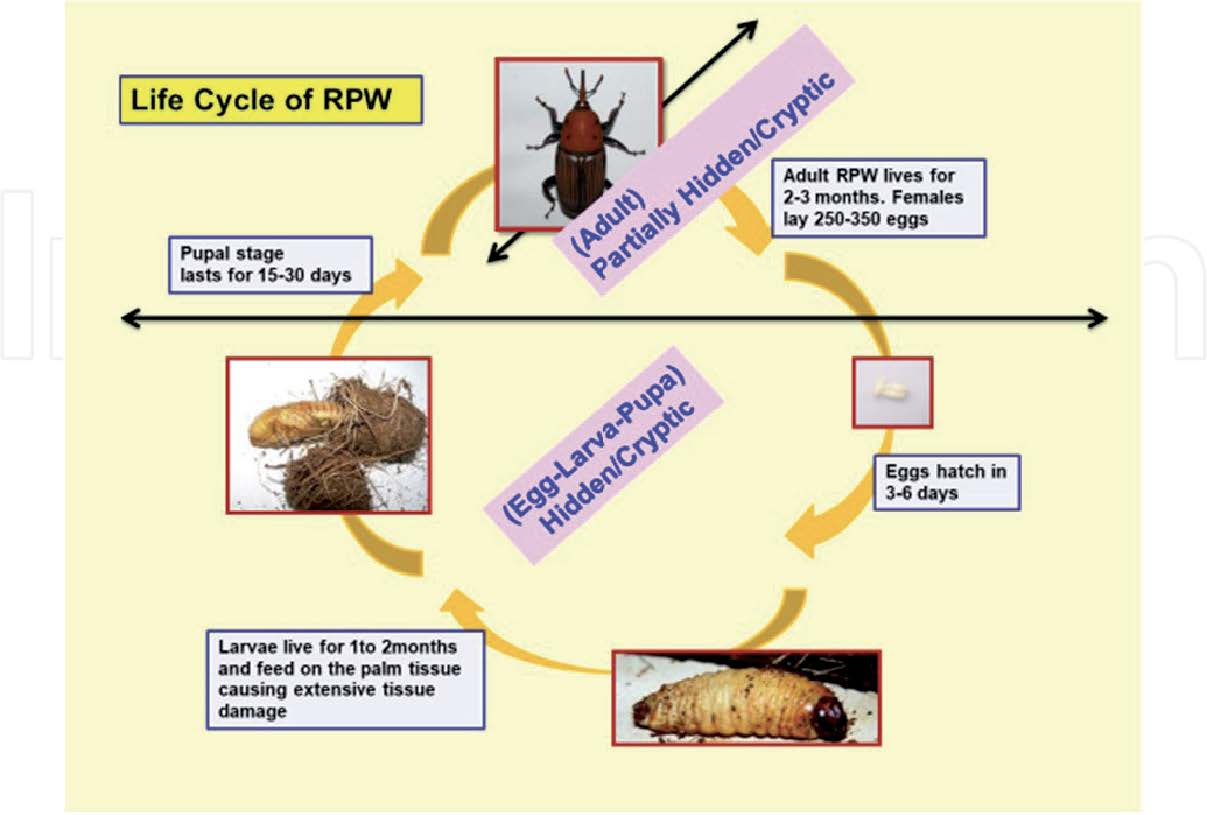
\includegraphics[width=0.75\textwidth]{figures/fig1_rpw_lifecycle.jpeg}
\caption{Schematic Diagram Depicting the Life Cycle of RPW \cite{alaufi2026}}
\label{fig:rpw_lifecycle}
\end{figure}
 
\begin{figure}[H]
\centering
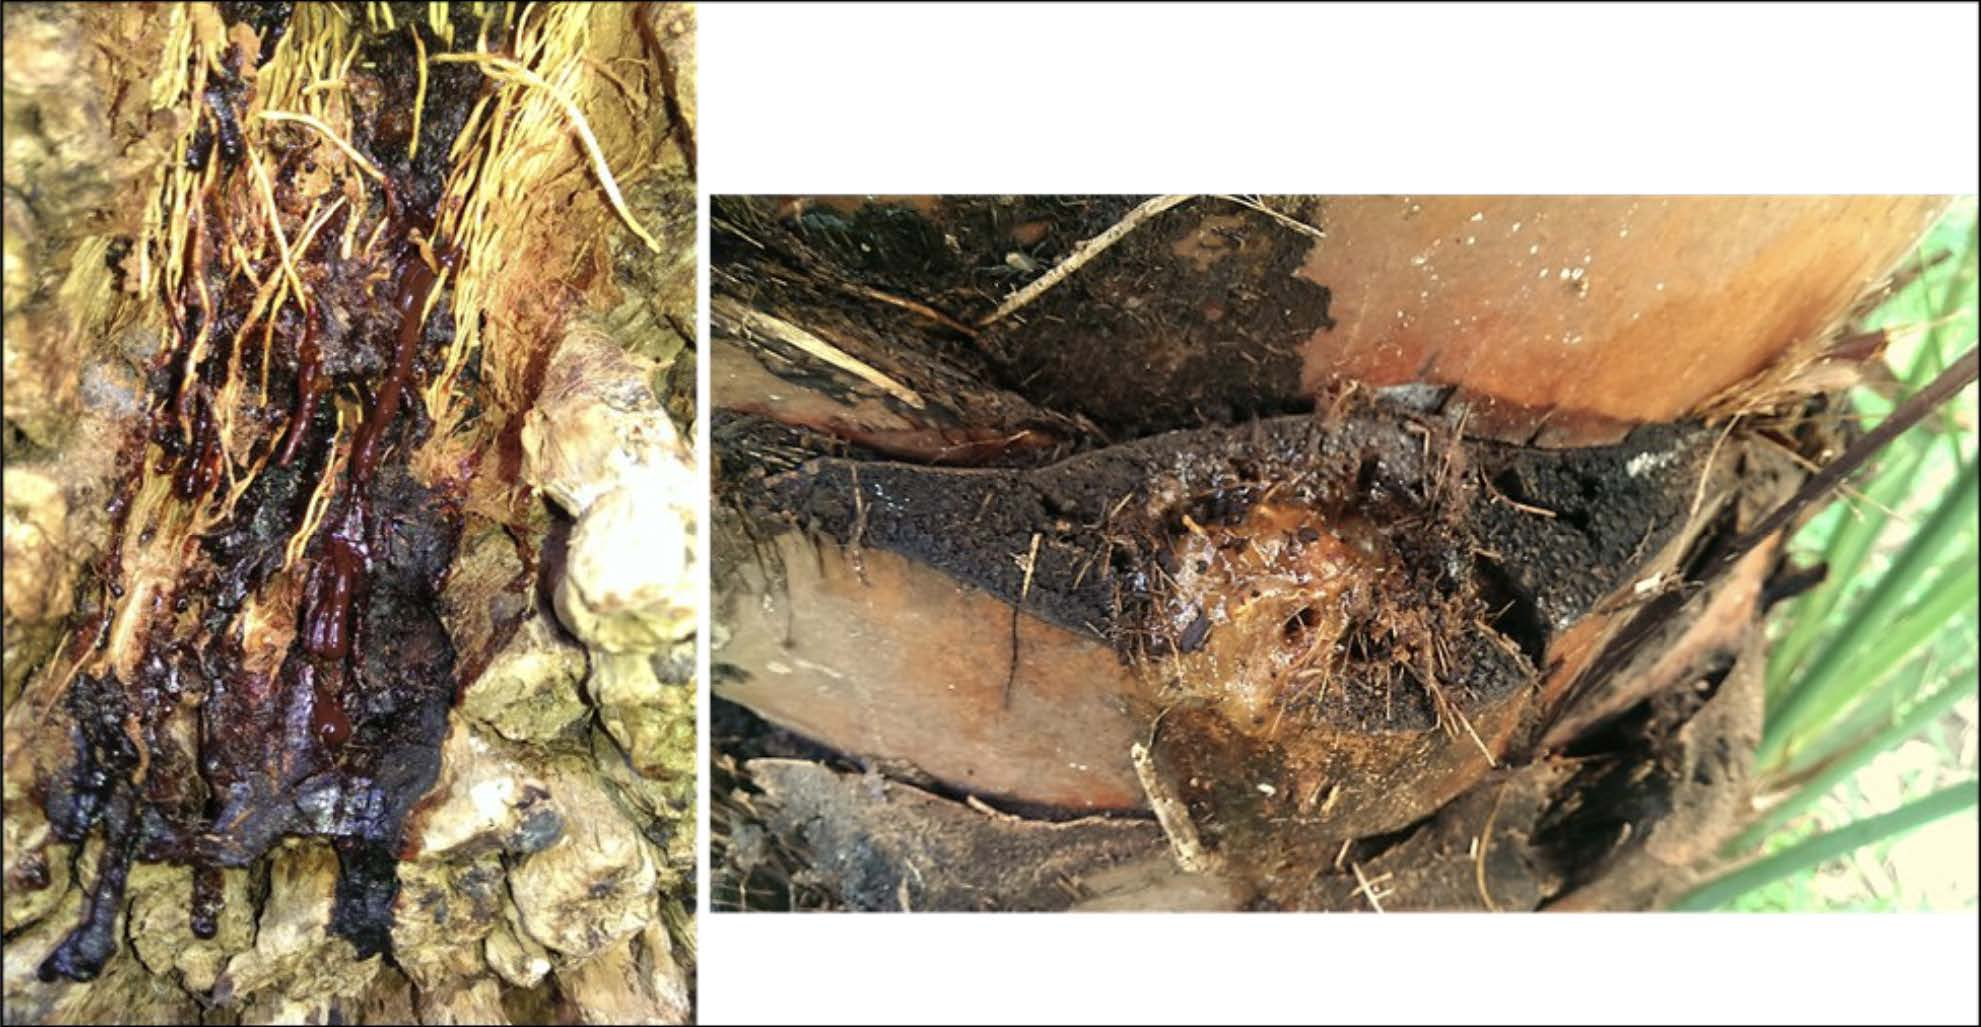
\includegraphics[width=0.75\textwidth]{figures/fig2_viscous_fluid.jpeg}
\caption{Viscous fluids ooze from the tunnels due to larvae inside the palm tree \cite{alaufi2026}}
\label{fig:viscous_fluid}
\end{figure}

\FloatBarrier
 
\subsection{Existing Solutions and Their Limitations}
 
Several methods have been explored to tackle the early detection of the RPW infestations, yet most existing approaches suffer from limitations related to scalability, invasiveness, cost, or detection accuracy. Visual and manual inspection remain the most adopted techniques; however, it is labor intensive, expensive, and subjective to the skills of the laborer. Even trained experts can inspect only a limited number of trees per day, and this method is particularly ineffective for detecting early-stage infestations due to the concealed larval activity inside the trunk \cite{saleem2022,alaufi2026}.
 
\begin{figure}[H]
\centering
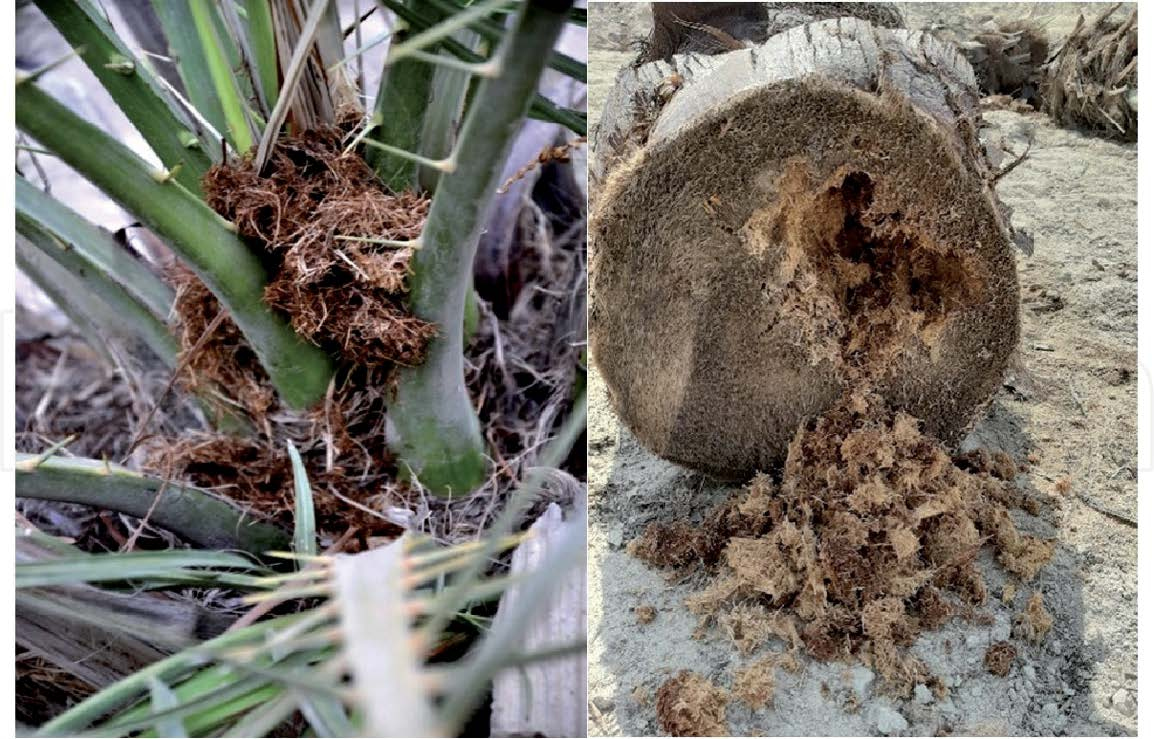
\includegraphics[width=0.75\textwidth]{figures/fig3_infected_crown.jpeg}
\caption{The crown of an infested young date palm (left) ejects chewed-up fibers. Internal palm tissue
shattered because of RPW Larvae consumption \cite{alaufi2026}}
\label{fig:infested_crown}
\end{figure}
 
Another standard method is to use pheromone trapping, which provides valuable information on adult weevil population trends and overall infestation pressure \cite{shukla2018,na2024}. However, traps only work on adult insects and yield no information about actual larval activity occurring inside the palm trees \cite{saleem2022}. Likewise, thermal imaging and remote sensing methods attempt to measure physiological stress signals or internal heat signatures, but these systems are frequently influenced by environmental conditions and generally provide lower reliability for large-scale field assessment than acoustic methods \cite{saleem2022,alaufi2026}. Conventional acoustic sensors are therefore a more promising early-warning approach \cite{karar2021,karar2022}. Piezoelectric probe-based devices are highly sensitive to larval gnawing sounds and, under controlled conditions, may detect infestations within the first two weeks of larval development \cite{ashry2020,ashry2022cnn}. Although such systems are typically invasive (e.g., they involve drilling the tree trunk) \cite{pinhas2008,karar2022}, they provide reliable and well-established detection performance. Despite their higher installation and maintenance costs, they remain suitable for targeted monitoring in semi-controlled environments \cite{karar2022}.

\begin{figure}[H]
\centering
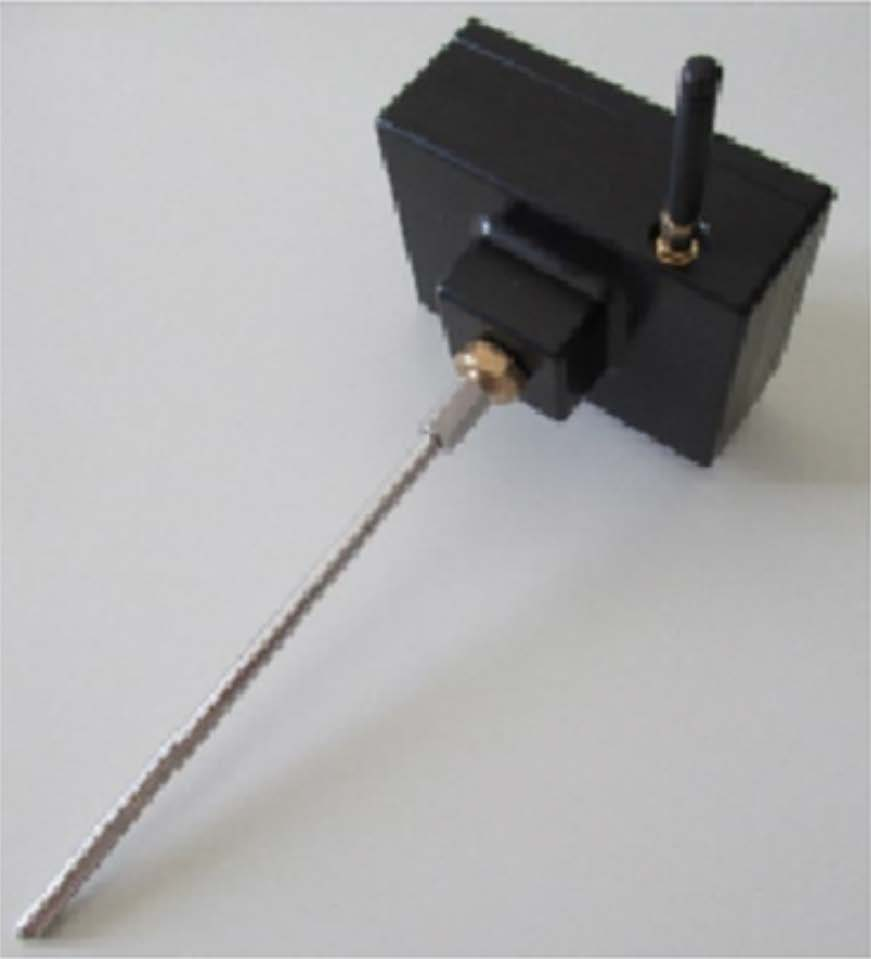
\includegraphics[width=0.5\textwidth]{figures/fig4_treevibes.jpeg}
\caption{TreeVibes sensing device for acquiring sounds of RPW larvae \cite{rigakis2021}}
\label{fig:treevibes}
\end{figure}
 
On the other hand, the combination of Distributed Acoustic Sensing (DAS) and Convolutional Neural Networks (CNNs) is the path with higher potential to meet project goals \cite{ashry2020,wang2021,ashry2022cnn}. DAS technology turns a conventional optical fiber into an external vibration sensor, allowing a single cable wrapped non-invasively around trunks to monitor many trees concurrently \cite{ashry2020,mao2021}. In conjunction with CNN-based classifiers, this method has reported classification accuracies between about 97\% and 99.9\% under controlled and semi-controlled studies \cite{wang2021,ashry2022cnn}. However, due to the high cost for installation, the focus will be on the implementation and evaluation of the conventional acoustic sensing approach as a practical and experimental solution.
 
 
 
\section{Project Description}
\label{sec:Description}
 
\earlierrevision{While DAS represents the highest-performing solution in the literature, its installation cost renders it impractical for large-scale deployment. This project aims to develop an affordable, IoT-based acoustic detection system for larvae (of RPW) in an early infestation stage. Instead of expensive distributed fiber-optic technology, the new system will be made from arrays of low-cost piezoelectric contact sensors mechanically coupled to palm trunks, capable of detecting internal vibrations produced by larval feeding and movement. By combining low-cost sensor devices, deep learning classifiers and cloud-based data analytics, this work intends to investigate a scalable and affordable open solution for real-time plantation monitoring at large-scale agroecological landscapes. The architecture follows a three-tier design: trunk-mounted piezoelectric sensing nodes transmit compact feature packets via LoRa to a cluster head, which aggregates and forwards data to a cloud backend for deep learning classification. The proposed system is intended to support earlier screening than visual inspection, subject to prototype and field validation \cite{ashry2020,ashry2022cnn,karar2022}. The system is designed around low-cost components, a modular IoT infrastructure, and automated analysis tools, to be low-cost and widely deployed. Thus, continuous remote monitoring could help reduce the considerable amount of field labor involved in pest control, and supply information to help reduce pesticide use, both of which would be helpful economically and environmentally \cite{saleem2022,karar2022}. As a secondary contribution, this project evaluates the recently introduced Mamba selective state-space model architecture for RPW acoustic classification, comparing it against established CNN and CNN-LSTM baselines.}

\newrevision{The baseline packet format is a design starting point, not a LoRa capacity claim. The project will compare it with smaller, versioned binary packets and report the measured payload size and airtime under the selected regional radio settings.}
 
\section{Problem Statement}
\label{sec:Statement}
 
\earlierrevision{Red Palm Weevil (RPW) is a destructive pest of palm species, particularly date palms in the Middle East and North Africa. Its larvae feed inside the trunk, where visual inspection cannot reliably detect early activity. When external symptoms such as holes, oozing sap, or crown collapse appear, internal damage may already be severe and treatment may be less effective \cite{saleem2022,ashry2022cnn}. This delay between infestation and visible detection can increase tree loss, treatment costs, and unnecessary pesticide use.}
 
\earlierrevision{This project addresses that gap by designing and validating a low-cost IoT system that monitors trunk vibrations produced by larval feeding and movement. Trunk-mounted piezoelectric sensors capture the vibrations, an ESP32 extracts compact acoustic features, LoRa carries the feature packets to a cluster head, and a cloud-based classifier distinguishes likely larval activity from environmental noise. The current mounting presses the sensor onto the palm surface using a plate; no drilled waveguide is planned. The intended outcome is an affordable and scalable early-warning system that supports inspection and treatment decisions before obvious external symptoms appear. The following section converts this problem into measurable design objectives.}

\newrevision{The project will also test whether packet compaction can reduce LoRa uplink cost without harming classification. Packet size, airtime, energy, memory, runtime, and classification performance will be measured before a communication benefit is claimed.}

\newrevision{A mechanically excited wood experiment is a bench-validation stage, not proof that the system detects live RPW larvae. If naturally infested palms are available, they will be tested separately. If they are unavailable, the project will use emulation and label all resulting conclusions as controlled bench validation.}
 
\section{Design Objectives}
\label{sec:Objectives}
 
\earlierrevision{The primary goal is to design, implement, and validate a low-cost IoT acoustic system for detecting RPW larval activity in palm trees before visible symptoms appear. The system combines minimally invasive trunk-mounted piezoelectric sensors with wireless communication and cloud-based classification. The following objectives define the project deliverables and how they will be evaluated.}
 
\subsection{Development of a Low-Cost Acoustic Sensing Unit}
 
\earlierrevision{The project shall build a trunk-mounted sensing-node prototype using a surface-contact piezoelectric element held by a plate, an ESP32, and a LoRa transceiver. The node shall sample at no less than 8 kHz, apply the defined preprocessing pipeline, and transmit test feature packets to the cluster head. Laboratory tests shall evaluate signal quality at increasing distances up to the literature-based 1.5--2.0 m range; that range will be reported as achieved only if the prototype demonstrates it. The actual project procurement costs are reported in Section~\ref{sec:Budget}; a per-node cost has not been established.}
 
\subsection{Implementation of Wireless Sensor Network Architecture}
 
The system shall establish a scalable Wireless Sensor Network architecture that supports simultaneous operation of multiple sensing nodes across a plantation. The network shall enable reliable transmission of acoustic data packets to a centralized cloud-based server with minimal data loss.
 
Power management shall be optimized to allow extended battery-powered operation using low-power electronics and duty-cycled deep sleep, with optional solar charging for long-term deployments. Each node shall be enclosed in a rugged outdoor casing to ensure environmental protection against heat, humidity, and dust. System performance shall be validated in terms of communication stability, node synchronization, and operational uptime under simulated field conditions.
 
 
\subsection{Development of a Deep Learning-Based Acoustic Classifier}
 
\earlierrevision{The project shall train and evaluate models that distinguish likely larval feeding sounds from wind, birds, machinery, and other background signals. Because missed infestations directly undermine early detection, model selection shall prioritize recall, with false-negative rate, precision, and F1 score reported as supporting metrics. Grouped 10-fold cross-validation shall report the mean and standard deviation of the primary metric, with recordings from the same tree or session kept within one fold. The target is a standard deviation below 3 percentage points.}
 
 
\subsection{Integration of Cloud-Based Data Processing and Monitoring Platform}
 
A centralized cloud infrastructure shall be developed to store, process, and analyze incoming MFCC feature streams transmitted by sensing nodes. The platform shall support automated validation, normalization, model inference, and alert generation when larval activity is detected. A user interface dashboard shall be implemented to provide plantation managers with real-time monitoring capabilities, including visualization of sensor status, detection events, and geographic mapping of suspected infestation zones. The system shall generate automated alerts through predefined communication channels when detection confidence exceeds a specified threshold.
 
\subsection{Validation Through Field Testing}
 
\earlierrevision{The complete system shall undergo field validation in the available plantation environment. Evaluation shall include recall, false-negative rate, precision, F1 score, false-positive rate, alert latency, packet loss, and system uptime over the observed monitoring period. Comparison with conventional inspection shall be reported only for the trees and dates actually observed; earlier detection will not be claimed without infestation-stage evidence. Results shall distinguish tested requirements from scalability and affordability targets that remain future work.}
 

\subsection{Deployment and Operational Integration}
 
\earlierrevision{The project shall produce guidance for expanding the validated prototype. It shall cover mounting and acoustic coupling, wireless checks, site-specific calibration, signal-quality verification, basic maintenance, node replacement, and troubleshooting. The guidance shall distinguish procedures demonstrated during the pilot from recommendations that still require commercial-scale validation. Large-farm coverage, minimal labor, and sustained field accuracy will remain future claims unless they are measured within the project.}
 
\section{Design Constraints}
\label{sec:Constraints}
 
In the context of deploying an acoustic microphone-based detection system for early Red Palm Weevil (RPW) detection, the following design constraints have been identified based on the technical limitations documented in the literature and the practical realities of real-world farm deployment.
 
\subsection{Environmental Noise Limitations}
 
A fundamental constraint of this project is the degradation in system performance under noisy outdoor conditions. Wind, rain, and ambient farm sounds such as bird activity and machinery generate acoustic interference that overlaps with the feeding frequency range of RPW larvae (100--2500 Hz), leading to a significant increase in false alarms. Contact microphone and piezoelectric probe systems are particularly susceptible to this interference when deployed in open-air environments, and no universal noise cancellation solution has been demonstrated to fully eliminate this limitation under all field conditions \cite{pinhas2008,karar2022,ashry2022cnn}.
 
\subsection{Restriction to Early-Stage Larvae Detection}
 
The acoustic microphone system is designed to detect RPW during the larval stage, specifically when larvae are actively feeding and producing chewing sounds inside the tree trunk. Adult weevils and eggs do not produce comparable acoustic emissions, which means the detection window is restricted to a narrow biological stage. Moreover, larvae do not produce feeding sounds continuously; intermittent feeding behavior reduces the reliability of single-measurement detection windows and may require extended monitoring periods to accumulate sufficient acoustic evidence of infestation \cite{sutanto2023,wang2021}.
 
\subsection{Invasiveness and Tree Integrity Constraints}
 
A significant practical constraint of probe-based acoustic systems is their invasive nature. Deploying piezoelectric contact microphones or waveguide rods typically requires drilling a small hole into the tree trunk to improve acoustic coupling between the sensor and the internal wood structure. This procedure risks introducing entry points for secondary pests, pathogens, and fungal infections, potentially causing additional harm to the trees being monitored. Repeated insertions across large plantations compound this risk and may be objectionable from an agronomic or regulatory standpoint \cite{pinhas2008,karar2022}.
 
\subsection{Sensor Coverage and Spatial Limitation}
 
The effective detection radius of a single piezoelectric or contact microphone probe is typically limited to approximately 1.5 to 2.0 meters from the insertion point \cite{pinhas2008,karar2022}. This means that taller trees or trees with large trunk diameters may require multiple sensors placed at different heights to ensure adequate coverage of the entire trunk volume where larvae may be present. Scaling this approach to large farms with hundreds or thousands of trees requires a proportional increase in the number of sensors, cabling, and wireless communication modules, significantly increasing infrastructure costs and deployment complexity \cite{pinhas2008,karar2022,saleem2022}.
 
\subsection{Computational and Real-Time Processing Constraints}
 
The machine learning models used for classification including Convolutional Neural Networks (CNNs), Bidirectional Long Short-Term Memory (Bi-LSTM) networks, and statistical models such as Gaussian Mixture Models (GMMs) require pre-trained weights and dedicated processing hardware. Feature extraction pipelines involving Mel-Frequency Cepstral Coefficients (MFCCs), Short-Time Fourier Transform (STFT) spectrograms, or Linear Predictive Coding (LPC) coefficients impose additional computational overhead. While classification accuracies exceeding 97\% have been reported under controlled laboratory conditions, extending these models to diverse real-world noise environments requires retraining on larger and more representative datasets, which may not be readily available \cite{boulila2023,karar2022,saranya2025}.
 
\subsection{Cost and Scalability Constraints}
 
Although individual piezoelectric sensors and microphone modules are relatively inexpensive compared to imaging technologies such as X-ray tomography, the requirement to assign at least one and often multiple sensors per tree, combined with the need for wireless communication nodes, power supplies, and data acquisition infrastructure, results in a total system cost that scales unfavorably with farm size. For large commercial plantations with thousands of trees, the cumulative hardware, installation, and maintenance costs may become prohibitive without institutional support or subsidy programs \cite{karar2022,saleem2022}.
 
\section{Project Impact}
\label{sec:Impact}
 
\subsection{Economic Impact}
 
\earlierrevision{RPW infestation causes substantial costs through lost production, treatment, removal, and replanting. Published estimates cited in this report include millions of US dollars in annual losses and a projected cost of about US\$235 million in Italy, Spain, and France by 2023 without effective containment measures \cite{ashry2020,saleem2022}. These figures describe the scale of the RPW problem; they do not establish the savings of the proposed system.}

\earlierrevision{The proposed system could reduce avoidable losses if earlier alerts help managers inspect and treat affected trees before removal becomes necessary. Its modular architecture also allows farms to add sensing nodes gradually instead of making a single large investment. However, the economic benefit must be demonstrated through field trials that compare equipment, installation, maintenance, cloud, and labor costs with the value of trees saved. The system is therefore expected to reduce reliance on repeated manual inspection, not eliminate inspection or labor entirely.}
 
\subsection{Societal Impact}
 
\earlierrevision{Date palms support food production, cultural heritage, and agricultural livelihoods across the Middle East, North Africa, and South Asia \cite{saleem2022}. Earlier detection of RPW can help protect productive trees and the communities that depend on them. Remote status information and automated alerts may also reduce the time workers spend on routine tree-by-tree screening, while directing trained staff to trees that require closer inspection.}

\earlierrevision{The system should support, rather than replace, farmers and pest-control specialists. Alerts are screening results, not final diagnoses, and field confirmation remains necessary before treatment. Adoption will also depend on affordability, reliable connectivity, straightforward training, and clear handling of farm location and operational data. These conditions are important so that the system remains useful to small farms as well as larger plantations.}

\newrevision{The same care is needed when presenting test results. A positive result from a wood-plank emulation is evidence that the apparatus and processing chain work under controlled conditions; it is not a diagnosis of a living palm. Keeping this distinction visible helps avoid false management decisions and unnecessary treatment.}
 
\subsection{Global Impact}
 
\earlierrevision{RPW has been reported in more than 60 countries, making earlier detection relevant to pest surveillance and containment beyond a single region \cite{ashry2022cnn,saleem2022}. A modular acoustic network may be adaptable to different plantations, but each deployment will require local validation because palm species, climate, noise, network coverage, and infestation patterns vary.}

\earlierrevision{The environmental benefit is also conditional. More precise alerts may support targeted inspection and treatment and may reduce unnecessary pesticide application, but the present project does not yet measure pesticide reduction, runoff, resistance, or other environmental outcomes. In addition, the proposed sensing nodes introduce batteries and electronic components that must be maintained and disposed of responsibly. The project therefore contributes a prototype for precision pest monitoring; broader environmental and biosecurity benefits must be confirmed through field deployment and lifecycle evaluation.}

\chapter{Literature Review}
\label{ch:Literature}

% ===============================
% CHAPTER 2: LITERATURE REVIEW
% ===============================

\section{Acoustic Transduction Methodologies}
\label{sec:GRP-I}

\earlierrevision{Acoustic detection uses vibrations produced when RPW larvae feed and move inside a palm trunk \cite{pinhas2008,karar2021}. Larvae fracture palm fibers and generate short, impulsive bursts that can differ from the background signals of a healthy tree \cite{pinhas2008,karar2021}. Because visible symptoms often appear only after substantial internal damage, these bursts can provide an earlier indicator of active larvae. Their presence alone is not a diagnosis, however, because environmental and biological noise can produce similar signals \cite{saleem2022,sutanto2023}.}

\subsection{Vibroacoustic Sensing Instruments and Hardware Configuration}

\earlierrevision{Common instruments include piezoelectric sensors and contact microphones coupled to the trunk \cite{pinhas2008,karar2021}. A piezoelectric sensor converts mechanical vibration into an electrical signal for sampling and analysis \cite{karar2021,saranya2025}.}

\earlierrevision{Unlike an air microphone, a contact probe is mechanically coupled to the trunk and is less exposed to airborne noise. Some implementations insert a metal waveguide, such as a rod or bolt, into a small drilled hole to improve coupling \cite{karar2021}. This can strengthen internal vibration measurements, but it makes the installation invasive and may still require site-specific noise control \cite{karar2021,sutanto2023}.}

\newrevision{Mechanical vibrational playback is an appropriate way to validate a contact-sensing path before field trials. Appel and Cocroft mechanically coupled piezoelectric actuators to plant leaves to replay feeding-related vibrations \cite{appel2014}. Escalante et al. used a piezoelectric actuator attached to a plant and calibrated a compensating filter for the test setup; their target was to keep frequency components within approximately $\pm3$ dB at the target \cite{escalante2024}. Piezoelectric actuator-to-solid-to-sensor arrangements are also established in structural-health monitoring, although this is only a methodological parallel and not biological evidence \cite{agis2020}.}

\newrevision{Accordingly, this project will use a vibration exciter mechanically attached to a wood plank, rather than an airborne speaker. The first bench stage will replay recordings through the attached exciter and measure the propagated vibration with piezoelectric sensors. It validates the apparatus and measurement method; it does not validate RPW detection in a living palm.}

\subsection{Signal Acquisition and Processing Techniques}

\earlierrevision{Larval signals are intermittent and often weak, so preprocessing is needed to separate likely feeding bursts from noise \cite{karar2021,saranya2025}. Studies use different sampling rates and filters; a commonly reported acoustic band is approximately 100--2500 Hz, although the appropriate range depends on the sensor and experiment \cite{karar2022,pinhas2008,saranya2025}.}

\earlierrevision{Feature extraction has been widely used to obtain compact spectral representations such as Mel-Frequency Cepstral Coefficients (MFCC), Bark Frequency Cepstral Coefficients (BFCC) and Linear Predictive Coding (LPC) \cite{saleem2022,saranya2025}. The Short-Time Fourier Transform (STFT) is often applied to convert time-domain signals into spectrogram images that visually represent energy distribution across frequencies \cite{karar2022,saranya2025}. These spectrograms are then used as inputs to machine learning classifiers, particularly Convolutional Neural Networks (CNNs), which learn to identify the distinct spectral-temporal patterns associated with larval feeding \cite{karar2022,saranya2025}. Architectures such as InceptionResNet-V2, MixConvNet, and Bidirectional Long Short-Term Memory (Bi-LSTM) networks have been explored for this purpose \cite{karar2021,karar2022,saranya2025}.}

\newrevision{LoRa payload limits depend on the regional plan and selected data rate, so a fixed payload capacity cannot be assumed \cite{lorawan2023}. The proposed communication study will compare the baseline feature packet with quantized MFCC features, compact metadata, and optional delta or run-length coding when those reduce size. Each variant will report payload bytes, airtime, packet loss, energy, and any change in classification performance.}


\subsection{Classification Performance and Experimental Accuracy}

\earlierrevision{Published classifiers report high accuracy within their own datasets and test conditions. MixConvNet achieved 97.38\% on a held-out test split of the public TreeVibes dataset, while its reported 10-fold cross-validation result was $95.90\% \pm 1.46\%$ \cite{karar2022}. Other studies report results above 97\% using concatenated cepstral features, BiLSTM models, or controlled laboratory recordings \cite{boulila2023,saranya2025,pinhas2008}. These values show that acoustic classification is feasible, but they are not directly comparable because the datasets, splits, sensors, noise conditions, and evaluation methods differ.}

\subsection{Advantages and Operational Limitations of Acoustic Detection Systems}

Acoustic sensing is valuable because controlled studies have detected young larvae before visible symptoms; one DAS experiment used larvae approximately 12 days old \cite{ashry2020}. Earlier detection may allow treatment while a tree is still recoverable \cite{saleem2022}. Low-cost contact sensors and embedded nodes may also be cheaper per measurement point than specialized optical or imaging equipment, although installation, maintenance, and the number of sensors required must be included in any deployment comparison.

However, there are several limitations hindering wide-spread deployment of probe-based acoustic systems. The need to drill in for the insertion of a waveguide introduces invasiveness and possibly provides entry points for other pests or pathogens \cite{karar2022}. Moreover, the detection radius of piezoelectric probes is usually about 1.5-2.0 m so that more than one sensor needs to be used for taller trees \cite{pinhas2008,karar2022}.

Environmental noise is still a challenge, and field studies have shown performance degradation under strong wind, heavy rain, and bird activity. From an operational point of view, the tools need to be installed and calibrated at each site, which may require substantial staff resources when setting up large commercial plantations \cite{karar2022,ashry2022cnn}.

\section{Distributed Acoustic Sensing (DAS) Methodologies} \label{sec:GRP-II}

Distributed Acoustic Sensing (DAS) measures the same larval vibration cues described above, but uses optical fiber instead of a separate electronic probe at each sensing point \cite{ashry2022cnn,wang2021}. This section therefore focuses on how DAS changes the coverage, installation, and processing of acoustic measurements rather than repeating the biological basis of detection.

\begin{figure}[H]
\centering
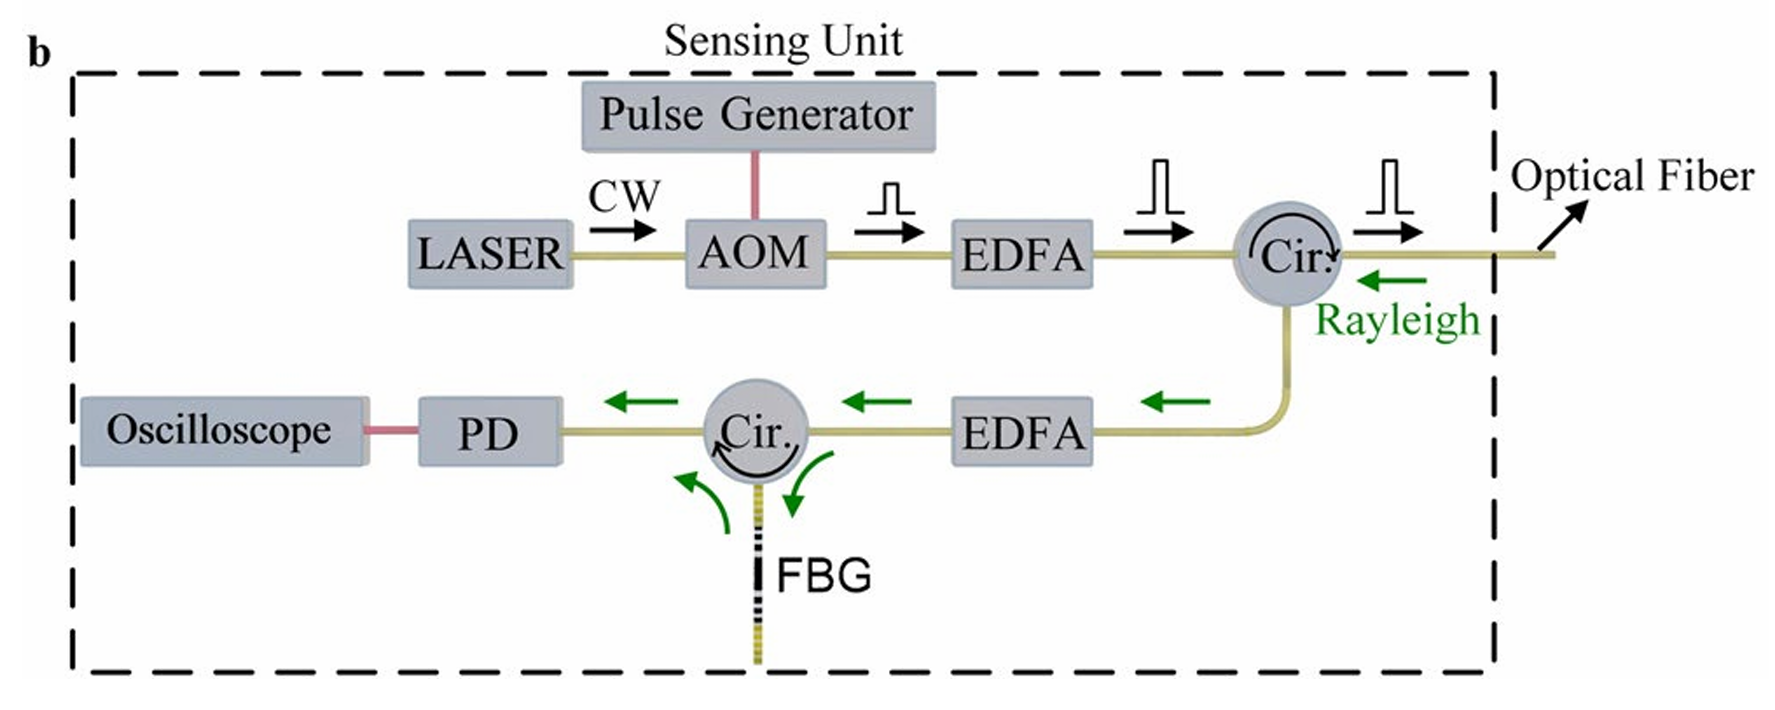
\includegraphics[width=0.75\textwidth]{figures/fig5_das_architecture.png}
\caption{DAS System Architecture \cite{wang2021}}
\label{fig:das_architecture}
\end{figure}

In phase-sensitive optical time-domain reflectometry ($\Phi$-OTDR), one continuous fiber is wrapped around the exterior of multiple trunks. A DAS interrogator measures changes in Rayleigh backscatter caused by local vibration and identifies the disturbance position along the fiber \cite{ashry2020,wang2021}. This provides distributed, non-invasive coverage without drilling each tree. Published work presents large-farm coverage as a design advantage, but the cited experiments do not demonstrate routine monitoring of 1,000 or more live trees; that scale should therefore be treated as projected capacity rather than validated deployment.

Signal processing in DAS-based systems follows a pipeline broadly analogous to that used in contact probe systems. Raw time-domain Rayleigh traces are differenced against a reference to extract acoustic perturbations, and a band-pass filter spanning 100 to 800 Hz is applied to suppress low-frequency environmental noise such as tree swinging caused by wind and high-frequency electronic noise from the sensing hardware, while preserving the dominant spectral content of larval feeding sounds \cite{ashry2022cnn,wang2021}. The filtered signals are then organized as two-dimensional matrices of spatial points versus temporal or spectral samples and passed to convolutional neural network (CNN) classifiers trained through supervised learning to distinguish infested from healthy tree signatures \cite{ashry2022cnn,wang2021,mao2021}.

Published DAS studies report strong signal-classification results within their experimental settings. Ashry et al. reported 97.0\% accuracy for temporal data and 97.1\% for spectral data using signals collected from controlled and outdoor-farm experiments \cite{ashry2022cnn}. Earlier laboratory work using simulated RPW sound also reported accuracies above 99\% \cite{wang2021}. Requiring temporal and spectral classifiers to agree reduced the reported false-alarm metric by about 20\% \cite{ashry2022cnn}. These metrics apply to the studied signals and conditions; they should not be interpreted as proven whole-farm detection accuracy.

A controlled indoor experiment detected larvae approximately 12 days old, and the later field study used larvae less than three weeks old \cite{ashry2020,ashry2022cnn}. DAS can be operated continuously, but outdoor performance remains sensitive to wind. The field study reported its best results below about 9 mph and substantially more false alarms at higher wind speeds \cite{ashry2022cnn}. Wider deployment therefore requires stronger field validation and improved handling of wind-induced vibration.

\section{Non-Acoustic Detection Methodologies}
\label{sec:GRP-III}

This section examines alternative sensing methodologies beyond acoustic detection. Prior studies have investigated a range of approaches, including chemical, molecular, and pheromone-based sensing techniques. Evaluating these alternatives was essential to ensure that the most appropriate sensing methodology was selected for the proposed system.

\subsection{Volatile Organic Compound (VOC) Biosensing}

Chemical detection strategies for \textit{Rhynchophorus ferrugineus} rely on the identification and sensing of volatile organic compounds and other biochemical signatures associated with larval feeding and metabolic activity within date palm tissues. These approaches exploit the fact that infestation induces measurable chemical changes in the host tree and that the insect itself emits characteristic volatile compounds during development.

A whole-cell bacterial biosensor was evaluated as a proof of concept for detecting volatile changes associated with RPW-infested material and date palms \cite{harpaz2022}. The genetically modified bacteria produced a bioluminescent stress response when exposed to air near tested samples. The study demonstrates that VOC-related biological responses can distinguish tested infested and uninfested samples, but it does not establish a field-ready sensor or identify a single infestation-specific compound. Commercial measurement equipment and controlled exposure were still required.

\begin{figure}[H]
\centering
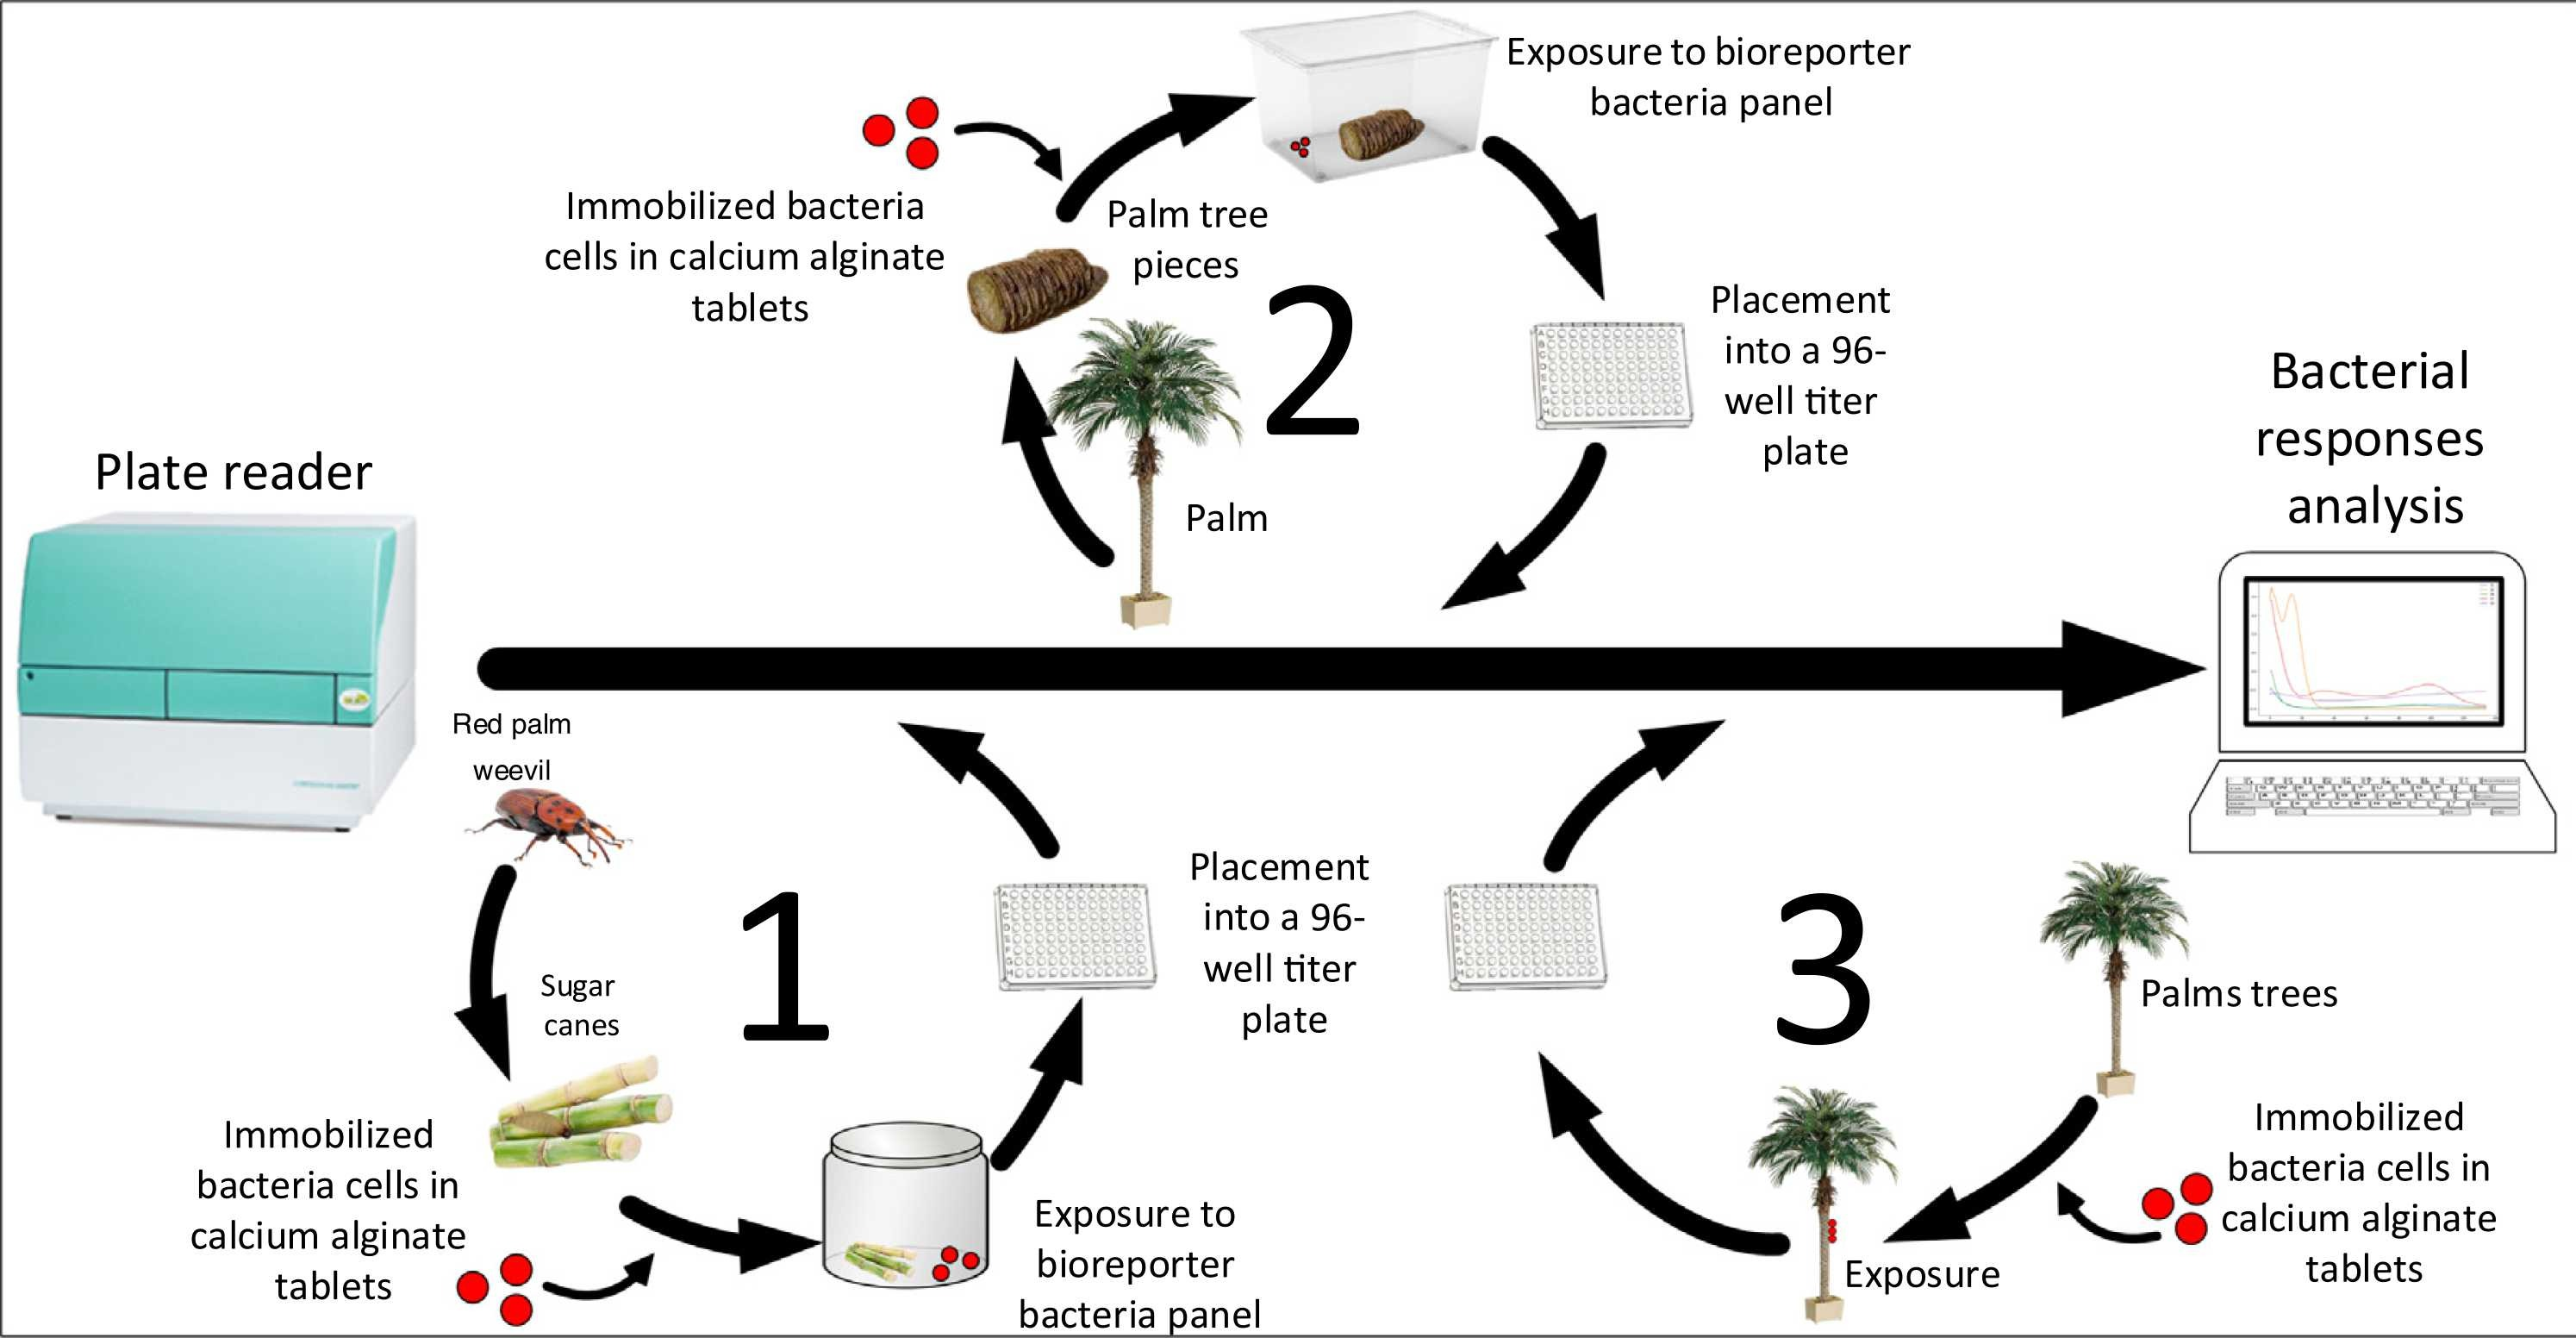
\includegraphics[width=0.99\textwidth]{figures/fig6_biosensor_schematic.png}
\caption{Schematic of The Experiment \cite{harpaz2022}}
\label{fig:biosensor_schematic}
\end{figure}

The chemical ecology of red palm weevil larvae further supports the feasibility of volatile-based detection. Detailed characterization of larval volatiles revealed stage-dependent emission profiles composed of specific chemical constituents that vary with developmental phase and pathogen stress \cite{ding2025}. The study identified distinct volatile organic compounds emitted by larvae and quantified their emission dynamics under varying biological conditions \cite{ding2025}. These findings indicate that larval metabolic processes generate a reproducible chemical fingerprint that can serve as a diagnostic indicator of infestation. Moreover, changes in volatile composition in response to physiological stress suggest that chemical emissions are sensitive to biological activity, potentially enabling differentiation between active and inactive infestations.

Together, volatile profiling and biosensing offer a possible route to non-destructive chemical screening \cite{harpaz2022,ding2025}. Their present maturity is limited: the cited work is proof-of-concept or laboratory research, and selectivity, sensor lifetime, calibration, field packaging, and false-positive control still require validation. The literature therefore supports VOC biosensing as a research alternative, not as an established continuous farm-monitoring method.

\subsection{Molecular Markers}

The cited molecular studies characterize RPW populations and support species identification; they do not directly detect hidden infestation inside a living palm. Molecular methods can confirm that a collected insect or biological sample belongs to \textit{Rhynchophorus ferrugineus}, but they first require representative material to be found and sampled.

Sabit et al. compared RPW samples from the Eastern Province of Saudi Arabia using RAPD and ISSR fingerprinting to study genetic relationships and possible population origins \cite{sabit2021}. The work is useful for population characterization and pest-management research, but it did not validate an assay for diagnosing infestation from palm tissue.

El-Zoghby et al. likewise examined genetic variability and ultrastructural traits in adult RPW collected from different locations in Egypt \cite{elzoghby2022}. Those results may inform later assay design, but the study addressed population differences and taxonomic characterization rather than early tree-level detection.

Molecular analysis may provide high-specificity confirmation when suitable biological material is available. However, the two cited studies do not support claims of low-level infestation detection, rapid screening of suspect trees, or portable on-site diagnosis. For this project, molecular methods are therefore considered a complementary confirmation approach rather than an alternative continuous-monitoring architecture.

\subsection{Pheromone Trap}

Pheromone-based detection exploits the aggregation behavior of \textit{Rhynchophorus ferrugineus}, which relies on chemical communication mediated by pheromones and synergistic attractants. By deploying optimized lure formulations and trap configurations, the presence of adult weevils in an area can be detected before widespread infestation occurs.

Optimization of pheromone trapping systems in Saudi Arabia demonstrated that trap performance is significantly influenced by lure composition, trap placement, and environmental factors \cite{shukla2018}. The study evaluated different trap contents and spatial arrangements, establishing conditions that maximize adult capture rates \cite{shukla2018}. Since adult weevils are responsible for dispersal and oviposition, their capture serves as an early indicator of infestation risk within a plantation. Effective trap optimization improves sensitivity, enabling detection of low-density populations.

Further assessment of attractant combinations in the United Arab Emirates examined the synergistic effects of pheromones with additional kairomonal components \cite{na2024}. The evaluation of different attractant mixtures demonstrated that specific combinations significantly enhance trap efficacy, increasing the probability of detecting active populations \cite{na2024}. Enhanced attractant formulations improve signal strength in surveillance programs by increasing adult aggregation around traps. This allows detection even when infestation levels are initially low.

\begin{figure}[H]
\centering
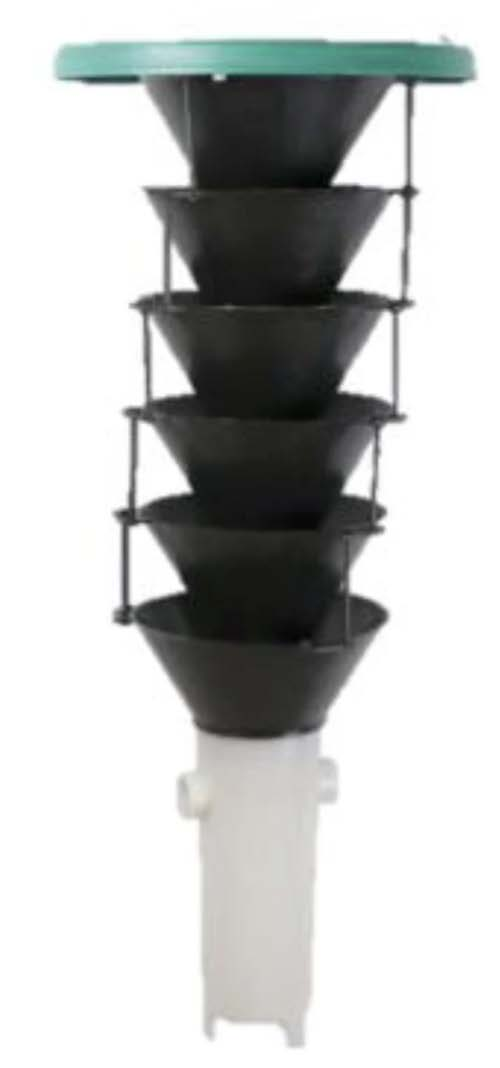
\includegraphics[width=0.2\textwidth]{figures/fig7_pheromone_traps.jpeg}
\caption{The Traps used in the Experiments \cite{na2024}}
\label{fig:pheromone_traps}
\end{figure}

Pheromone trap systems function as indirect detection mechanisms by capturing dispersing adults, thereby providing spatial information about infestation hotspots. Data collected from optimized traps can be used to map population distribution and monitor seasonal dynamics. The combined findings from trap optimization studies and attractant assessment experiments demonstrate that chemical communication pathways can be systematically leveraged for surveillance \cite{shukla2018,na2024}. Properly calibrated pheromone trapping networks enable early identification of infestation zones, facilitate targeted intervention, and support continuous monitoring of red palm weevil activity.

\section{Signal Processing Algorithms for Acoustic Data Processing of RPW}

The reliable detection of Red Palm Weevil (RPW) larvae through acoustic sensing depends not only on the quality of the hardware used to capture vibrational signals, but critically on the signal processing pipeline applied to raw acoustic data. Because larval feeding sounds are low-amplitude, intermittent, and embedded within a background of environmental noise, a sequence of carefully designed processing stages is required to extract meaningful features from the raw signals. The literature identifies a consistent pipeline consisting of preprocessing and filtering, followed by time-frequency feature extraction.

\subsection{Preprocessing and Bandpass Filtering}

Raw acoustic signals captured by piezoelectric contact microphones or similar transducers are typically sampled at rates ranging from 8 kHz to 44 kHz. Prior to any feature extraction, the signals undergo digital bandpass filtering to isolate the frequency of band of interest and suppress noise sources that fall outside the larval acoustic signature. The commonly applied bandpass range spans 100 to 2500 Hz, which encompasses the dominant chewing and movement sounds produced by RPW larvae while rejecting low-frequency interference such as wind-induced vibrations, ground tremors, and machinery noise below 100 Hz, as well as high-frequency electronic noise above the band of interest \cite{pinhas2008,rach2013}. This filtering stage is foundational to all subsequent processing steps, as it directly determines the signal-to-noise ratio of the features passed to any downstream analysis.

\subsection{Signal Squaring and Moving Average}

Following bandpass filtering, a common energy-based processing step involves squaring the time-domain signal to convert it into a strictly positive power envelope, which accentuates the amplitude differences between larval activity bursts and background noise. A moving average is then applied to the squared signal over a sliding time window typically 100 ms to smooth instantaneous noise spikes and reveal the underlying temporal pattern of larval feeding activity. This approach exploits the on/off feeding behavior of RPW larvae, which produces characteristic ups and downs in the moving average output when larvae are active, in contrast to the relatively flat and constant moving average observed from healthy trees. The complete signal processing pipeline, from raw signal acquisition through to the final infestation decision, is illustrated in Figure~\ref{fig:signal_pipeline} \cite{wang2021}.

\begin{figure}[H]
\centering
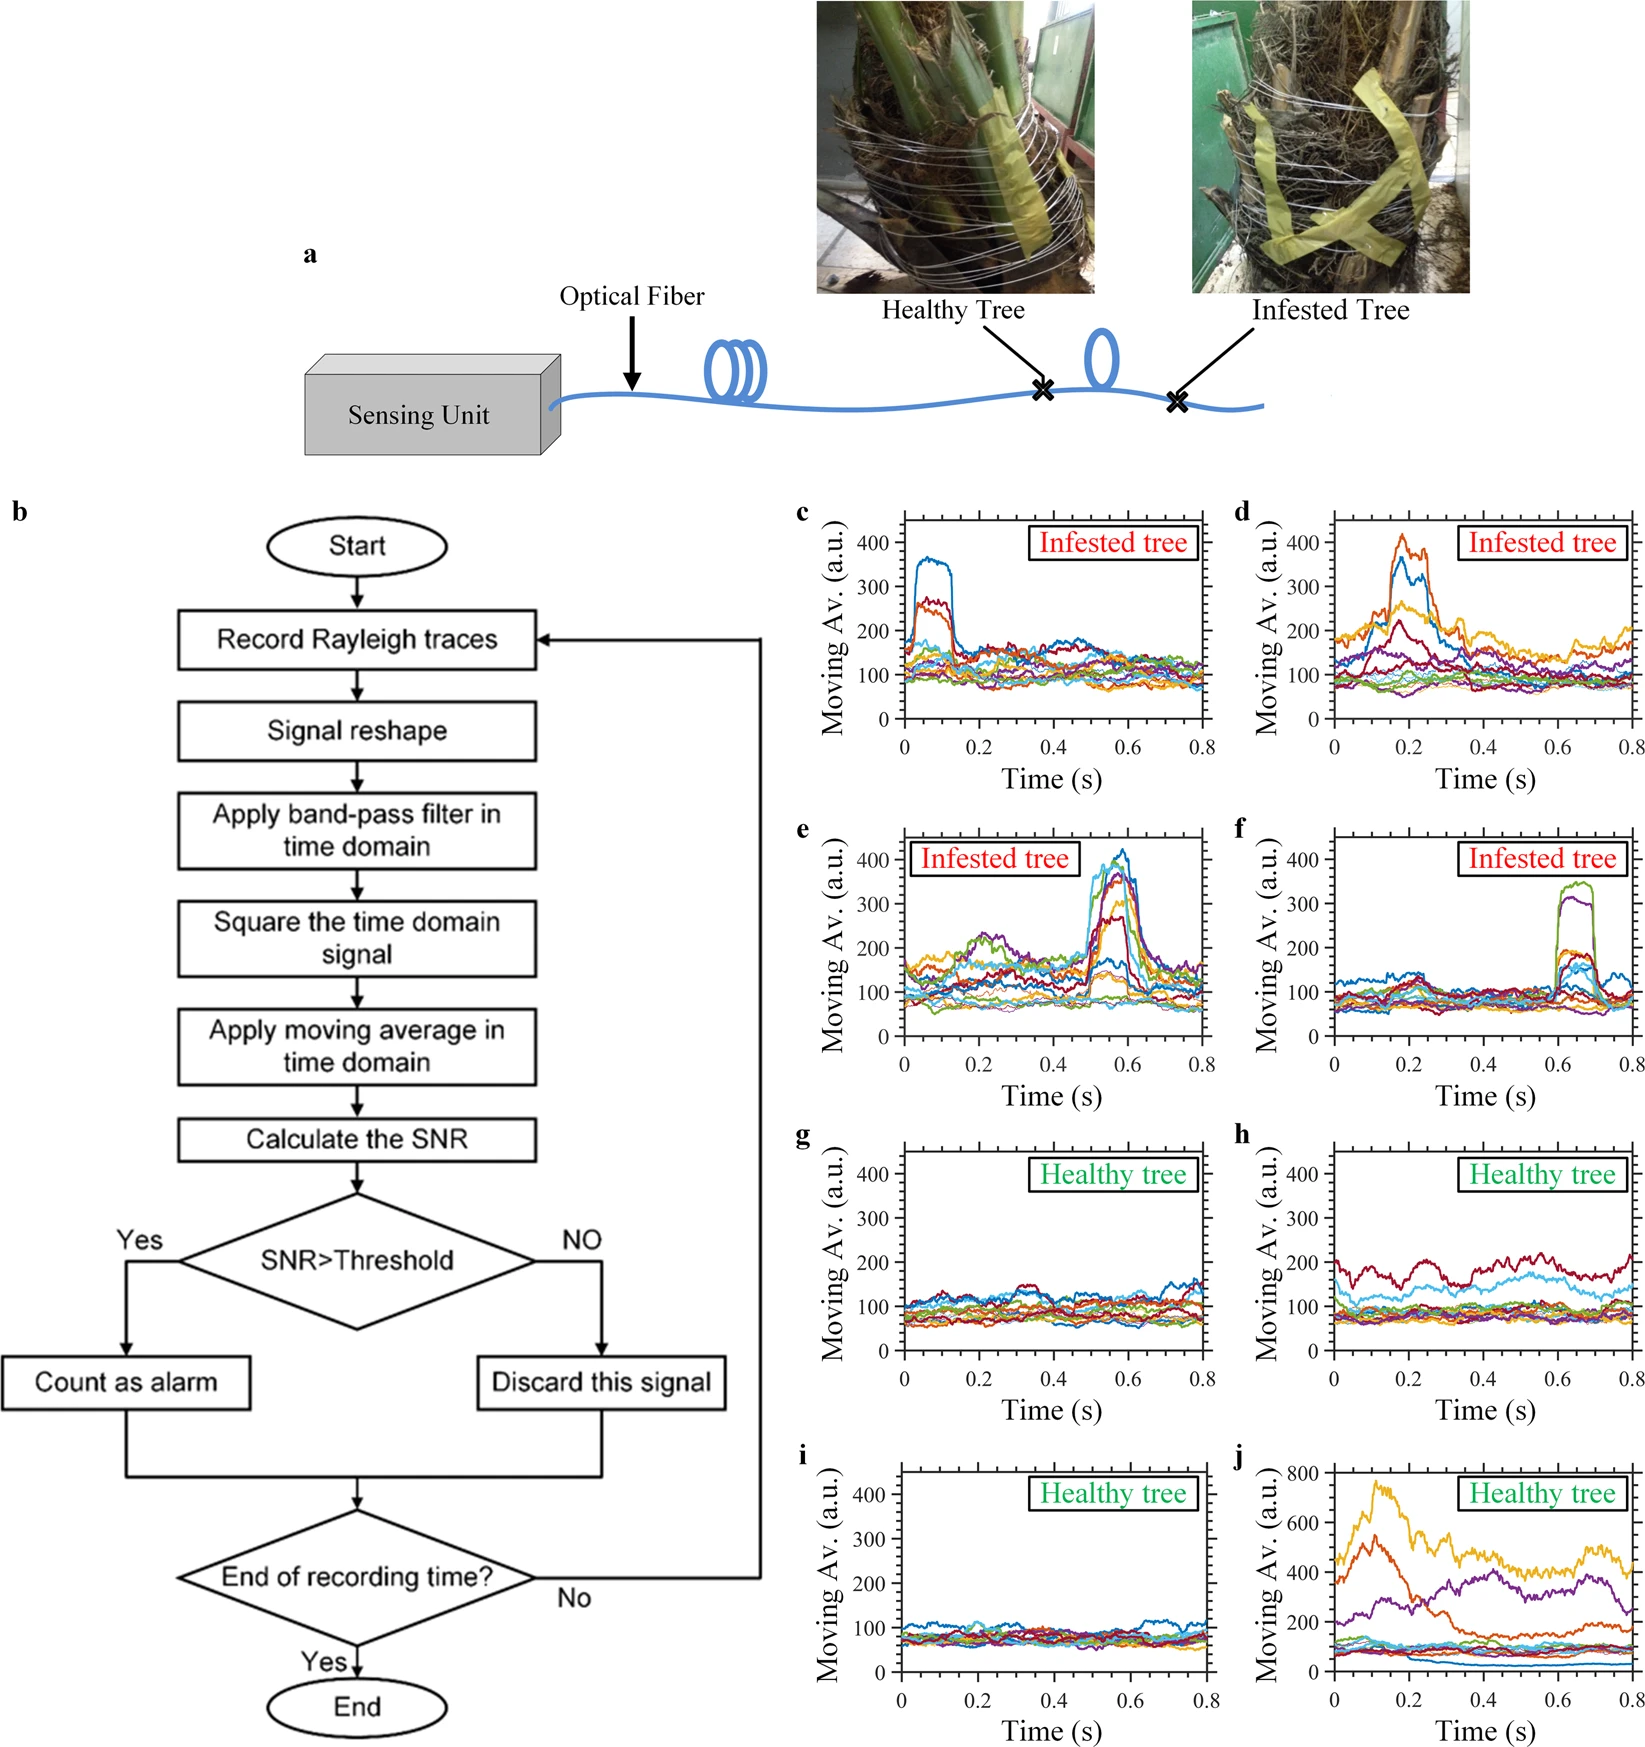
\includegraphics[width=0.99\textwidth]{figures/41598_2020_60171_Fig4_HTML.png}
\caption{Flowchart of the signal processing and detection algorithm \cite{ashry2020}}
\label{fig:signal_pipeline}
\end{figure}

\subsection{Signal-to-Noise Ratio Thresholding}

After the moving average is computed, an SNR-like measure compares its high and low levels within each window. A window above the selected threshold is counted as an infestation alarm. The threshold must be calibrated for the sensor and environment rather than treated as universal. In one controlled DAS experiment, a 4 dB threshold produced 97 alarm counts for an infested tree and 9 for a healthy tree during a two-hour recording \cite{ashry2020}.

\subsection{Short-Time Fourier Transform and Spectrogram Representation}

A widely adopted alternative approach for converting time-domain acoustic signals into a form suitable for further analysis is the Short-Time Fourier Transform (STFT). The STFT divides the filtered signal into short, overlapping temporal windows and computes the Fourier transform of each window, yielding a two-dimensional time-frequency representation known as a spectrogram. The spectrogram encodes how the energy distribution across frequencies evolves over time, revealing the characteristic intermittent burst patterns associated with larval feeding \cite{pinhas2008,rach2013}. This representation is particularly valuable because it preserves both the spectral content and the temporal structure of the acoustic signal simultaneously, making the distinct impulsive nature of larval chewing sounds visually and mathematically distinguishable from more continuous environmental noise sources. Deep learning models applied to spectrogram inputs have demonstrated strong classification performance for RPW detection, with studies reporting accuracies exceeding 97\% under controlled conditions \cite{boulila2023}.

\subsection{Cepstral Feature Extraction}

An alternative and complementary approach to spectrogram-based representation is cepstral feature extraction. Mel-Frequency Cepstral Coefficients (MFCCs) compress the spectral content of an acoustic signal into a compact vector representation by mapping the power spectrum onto the mel frequency scale a perceptual scale that approximates the non-linear frequency response of the human auditory system and then applying a discrete cosine transform. Similarly, Bark Frequency Cepstral Coefficients (BFCCs) apply the same principle using the Bark psychoacoustic scale, and Constant Q Cepstral Coefficients (CQCCs) use a constant-Q frequency resolution that provides higher frequency resolution at lower frequencies. All three representations produce compact, noise-robust spectral descriptors that suppress redundant fine spectral detail while retaining the envelope shape most characteristic of the acoustic source \cite{pinhas2008,rach2013,boulila2023}. Studies have shown that concatenating MFCC, BFCC, and CQCC features before classification outperforms using any single feature extraction technique in isolation, yielding superior results across multiple acoustic datasets \cite{boulila2023}. Linear Predictive Coding (LPC) offers a further alternative, modeling the acoustic propagation channel through the wood structure as an autoregressive filter whose coefficients summarize the spectral envelope of the signal in a small set of parameters. LPC is computationally efficient and has been shown to effectively capture the resonance characteristics of larval feeding sounds as they propagate through palm trunk tissue \cite{saranya2025}.

\subsection{Comparative Assessment}

Each feature extraction approach involves trade-offs between computational complexity, compactness, and robustness to environmental noise. The SNR-based moving average approach is computationally lightweight and well-suited to real-time embedded deployment but is most effective when larval feeding produces clearly intermittent amplitude patterns and may be susceptible to false alarms under highly variable noise conditions \cite{wang2021}. STFT spectrograms preserve the most complete time-frequency information but produce large two-dimensional representations that carry higher computational cost in downstream processing \cite{boulila2023}. Cepstral features such as MFCCs, BFCCs, and CQCCs are significantly more compact and computationally lighter, and their combination has demonstrated particularly strong generalization across different acoustic environments \cite{boulila2023}. LPC coefficients are the most compact representation and least computationally demanding, making them attractive for embedded or IoT-constrained deployment scenarios \cite{saranya2025}. For real-world farm deployment, where wind, rain, bird activity, and mechanical noise are unavoidable, selecting the appropriate feature representation for the prevailing noise environment is a critical design decision that directly affects detection reliability \cite{pinhas2008,rach2013,saranya2025}.

\section{Deep Learning for Acoustic Data Classification of RPW Infestation}

\subsection{CNN Transfer Learning for Acoustic Signal Classification}

Transfer learning allows a CNN pre-trained on a large image dataset to classify image-like acoustic representations with less task-specific data. Karar et al. applied InceptionResNet-V2 to TreeVibes and reported 97.18\% accuracy on their train/test split and $94.53\% \pm 1.69\%$ under 10-fold cross-validation \cite{karar2021}. 

In another study, the authors improved this approach by applying audio feature extractors to the raw audio signal before feeding the extracted features into transfer learning CNN models \cite{boulila2023}. The selected audio features were Mel-frequency cepstral coefficients (MFCC), Constant Q cepstral coefficients (CQCC), and Bark frequency cepstral coefficients (BFCC). Each of these feature extraction techniques generates a two-dimensional image representing the extracted features. These three feature images are concatenated and fed into one of the following transfer learning (TL) models: MobileNetV2, ResNet50V2, ResNet152V2, VGG16, VGG19, DenseNet121, DenseNet201, Xception, and InceptionV3.

The final feature vector output by a TL model is then fed into a classifier to determine whether the palm tree is infested. A research paper provided the following diagram to illustrate the full pipeline, from the audio signal to classification \cite{boulila2023}.

\begin{figure}[H]
\centering
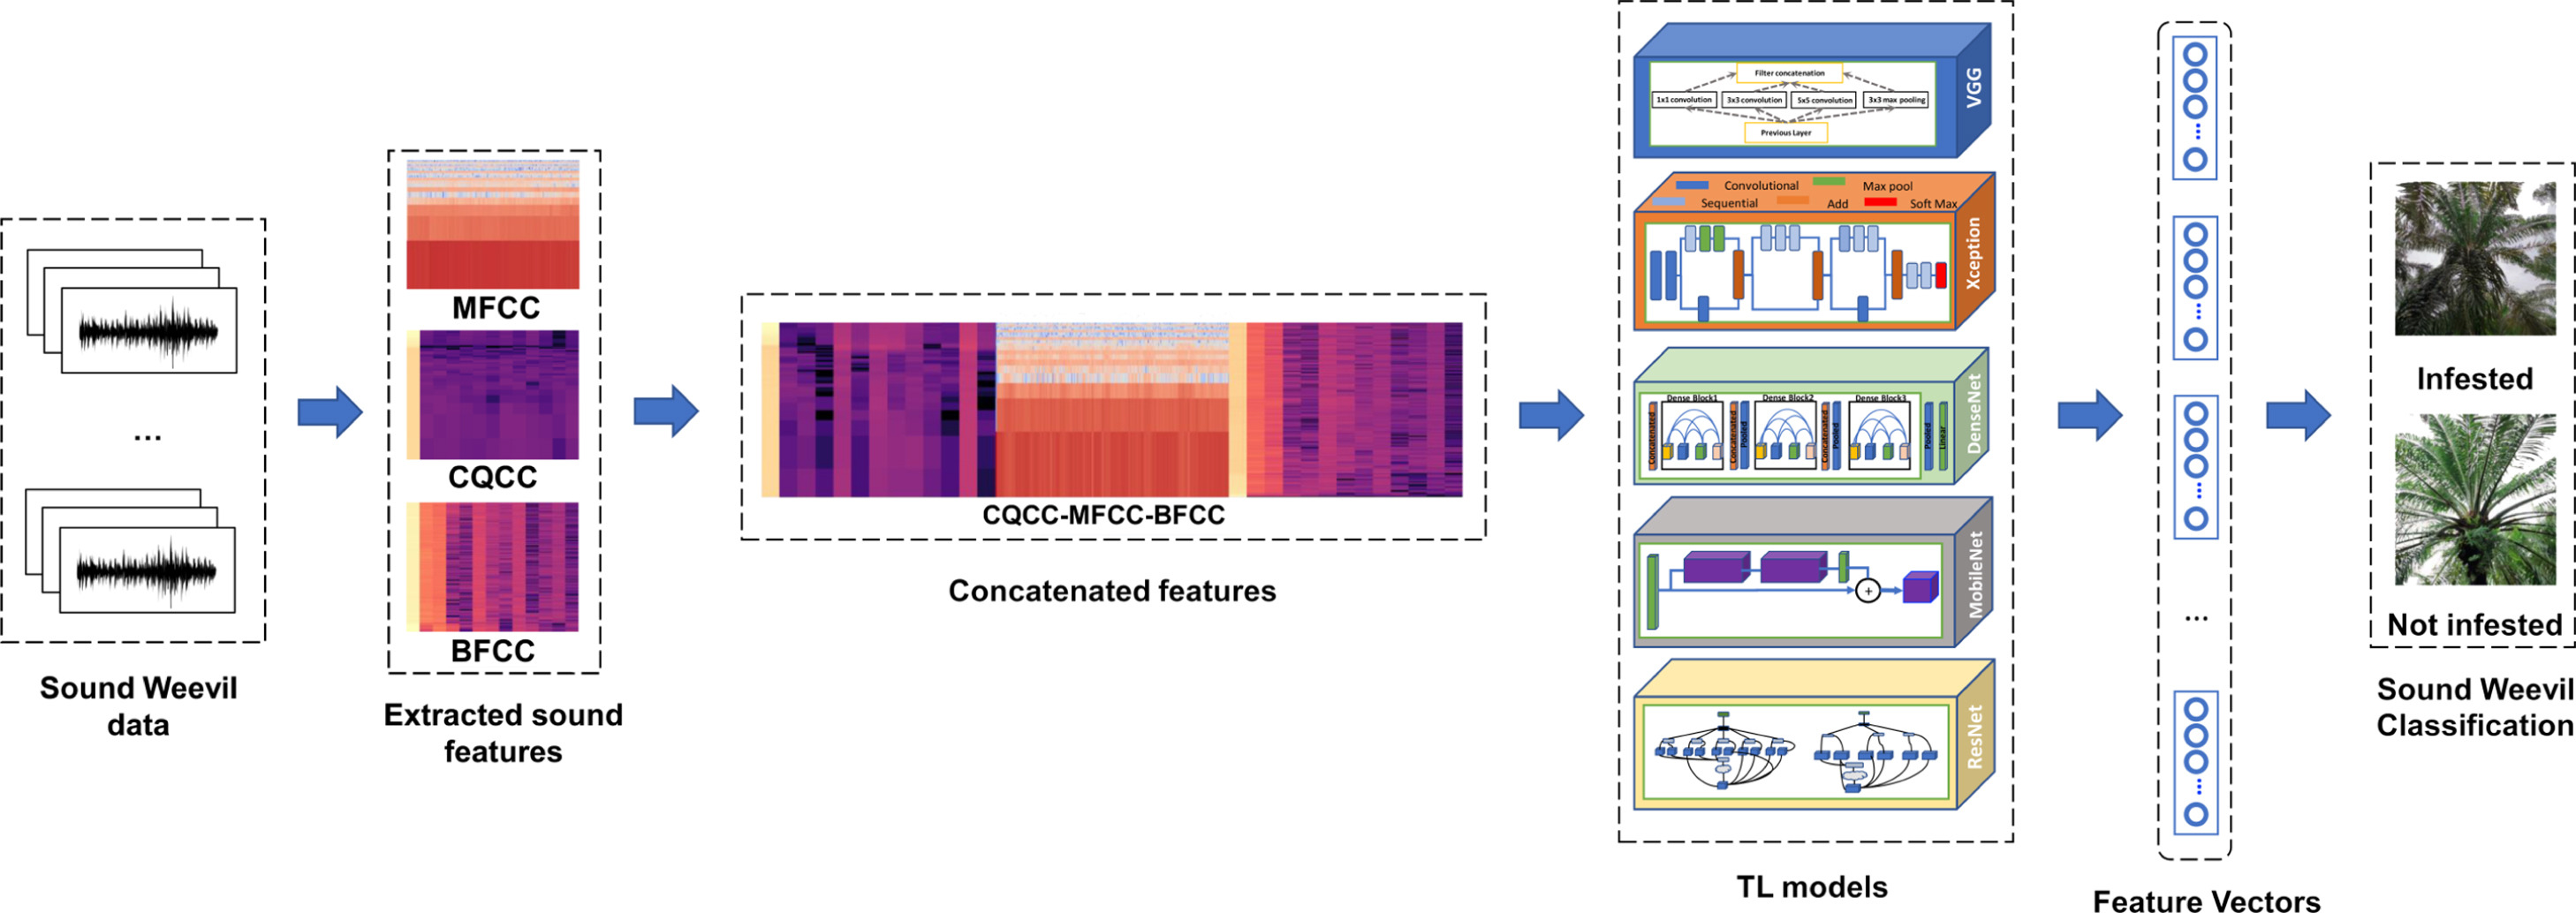
\includegraphics[width=0.99\textwidth]{figures/fig9_cnn_pipeline.jpg}
\caption{Full Model Pipeline \cite{boulila2023}}
\label{fig:cnn_pipeline}
\end{figure}

On the RPW dataset used by Boulila et al., combined CQCC, MFCC, and BFCC images generally outperformed single-feature inputs across the evaluated CNNs \cite{boulila2023}. The same feature combination achieved 0.95 accuracy, 0.947 precision, 1.0 recall, and a 0.973 F1 score on ESC-10 \cite{boulila2023}. Results on general environmental-sound datasets support the feature-fusion method, but they are not direct evidence of RPW field performance.

These results make cepstral feature fusion with transfer-learning CNNs a reasonable candidate for comparison in this project. Its value must still be tested on representative RPW field recordings with tree-level data separation.

\subsection{Bidirectional Long Short Term Memory Models for RPW Detection Through Acoustic Detection}

Another paper proposed a Bidirectional Long Short-Term Memory (BiLSTM) architecture for detecting RPW infestation from acoustic signals \cite{saranya2025}. The study introduced a complex, multistage data preprocessing pipeline, beginning with initial noise suppression to remove environmental noise such as wind. This is followed by Linear Predictive Coding (LPC), which extracts ``compact and discriminative'' spectral features from the audio signals that are specific to RPW activity.

Next, cosine similarity is computed between the extracted features and reference RPW and non-RPW vectors. The resulting cosine similarity coefficients are stored in a matrix, where each row corresponds to an audio file and each column contains similarity values. This matrix is then fed into a Bidirectional LSTM architecture, meaning that the temporal signal is processed by both a conventional forward LSTM and a backward (end-to-start) LSTM. The outputs of the forward and backward LSTMs are concatenated and passed to a dense layer for classification.

The researchers reported a classification accuracy of 98.02\%. They attributed the success of this approach in noisy environments to the ``combination of LPC feature extraction, cosine similarity-based feature matching, and a Bi-LSTM architecture.''

\subsection{Comparing RNNs and CNNs}

The researchers compared the use of CNNs and LSTM-based RNNs for environmental audio classification using the FSDKaggle2018 and ESC-50 datasets \cite{rezaul2024,fonseca2018}. Mel Frequency Cepstral Coefficients (MFCC) were used as a feature extractor, and the resulting feature vectors were fed into either a CNN or an LSTM model.

The ESC-50 CNN architecture used consisted of 10 layers, including convolutional layers with varying numbers of filters (ranging from 16 to 128), a filter size of 3, and ReLU activation, along with max-pooling, dropout, and dense layers for classification \cite{rezaul2024}. The LSTM architecture for ESC-50 consisted of 13 layers, including ``LSTM units, Batch Normalization, and Dropout layers.'' Time-distributed dense layers were also used, followed by a dense multi-class classifier layer.

The researchers reported that CNNs performed better than LSTMs on the smaller FSDKaggle2018 dataset, achieving 96.52\% and 87.88\% test accuracy, respectively \cite{rezaul2024,fonseca2018}. However, LSTMs performed better on the ESC-50 dataset, achieving 92.89\% accuracy compared to 88.47\% for CNNs \cite{rezaul2024}.

\subsection{CNN-LSTM Hybrid Architecture}

Another study proposed a hybrid CNN-LSTM model for environmental audio classification. This architecture uses 1D CNNs as feature extractors and feeds the extracted features into an LSTM block to capture time-based sequential relationships. A fully connected layer is then used for classification. Dropout layers are applied before the LSTM layer and before the fully connected layer. Max-pooling and ReLU activation are used after each convolutional layer. Figure~\ref{fig:cnn_lstm} illustrates the hybrid CNN-LSTM architecture presented in \cite{akter2025}.

\begin{figure}[H]
\centering
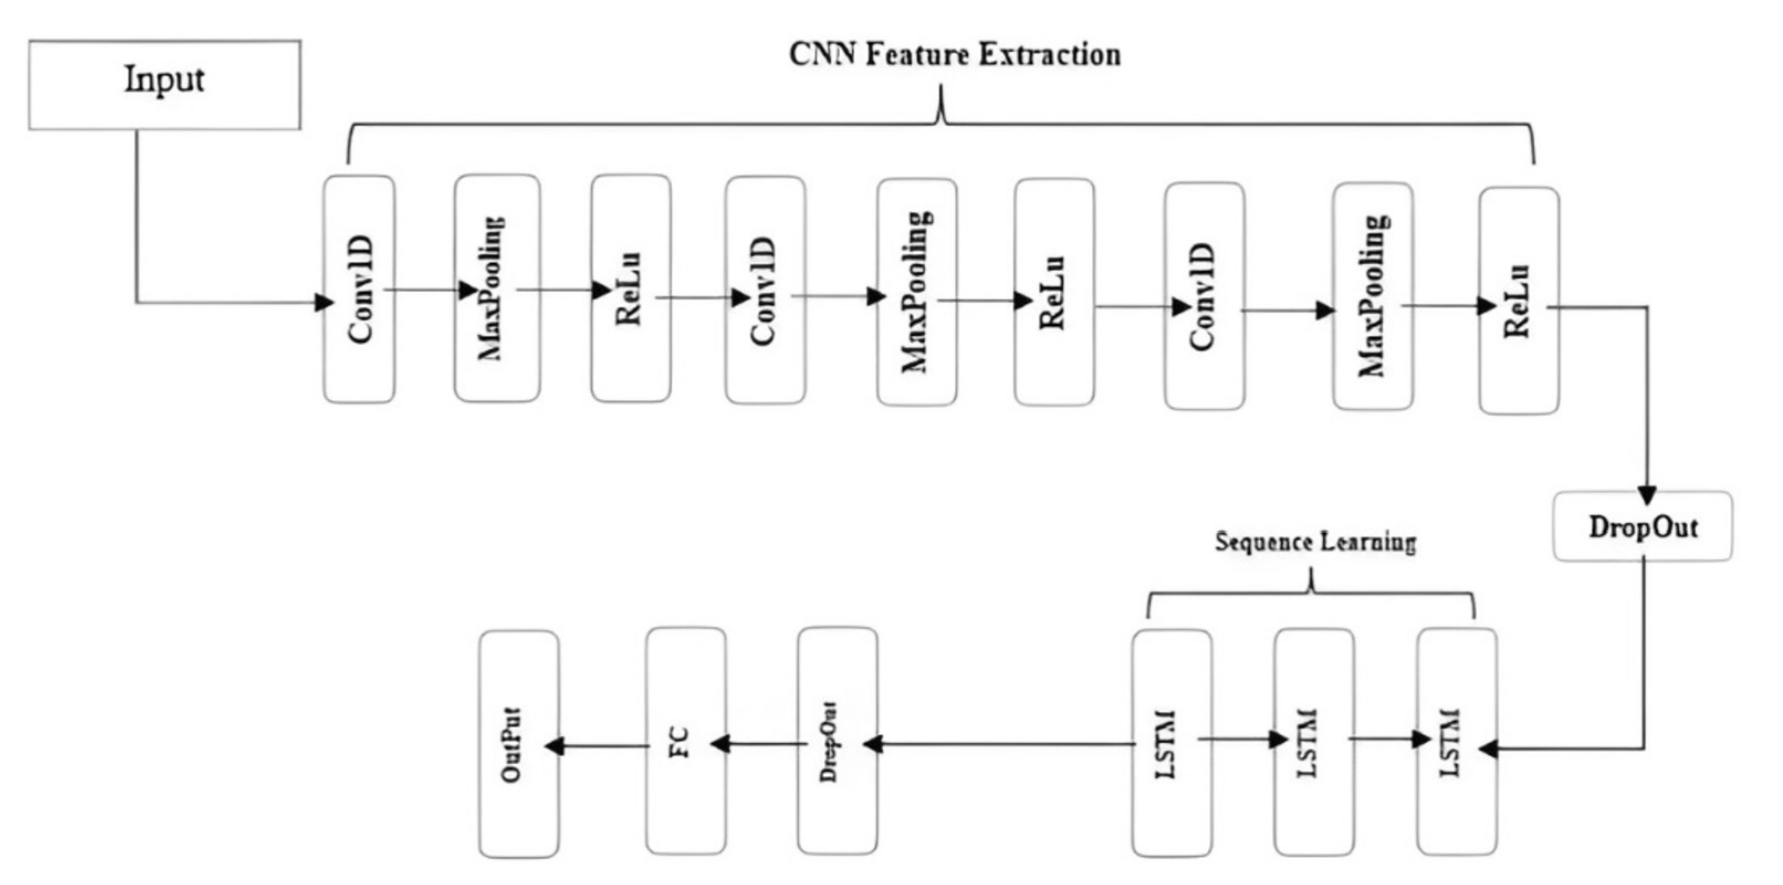
\includegraphics[width=0.85\textwidth]{figures/fig2_6_replacement.png}
\caption{CNN-LSTM Hybrid Model Architecture \cite{akter2025}}
\label{fig:cnn_lstm}
\end{figure}

The model reported 99.33\% accuracy on ESC-50 and 98.38\% on UrbanSound8K \cite{akter2025}. These are environmental-sound results, not RPW results. They justify evaluating a CNN-LSTM baseline, but they do not show that the same accuracy will transfer to trunk vibrations. Combining that architecture with the MFCC, BFCC, and CQCC features studied by Boulila et al. is a testable project hypothesis rather than an established improvement \cite{boulila2023}.

\renewcommand{\arraystretch}{1.1}
\begin{landscape}
\scriptsize
\renewcommand{\arraystretch}{1.3}
\setlength{\tabcolsep}{6pt}

% Center the longtable on the page
\setlength\LTleft{\fill}
\setlength\LTright{\fill}

\begin{longtable}{@{}
    >{\raggedright\arraybackslash}p{2.8cm}
    >{\centering\arraybackslash}p{1.0cm}
    >{\raggedright\arraybackslash}p{1.8cm}
    >{\raggedright\arraybackslash}p{2.5cm}
    >{\raggedright\arraybackslash}p{9.5cm}
    >{\raggedright\arraybackslash}p{1.6cm}
    >{\raggedright\arraybackslash}p{2.0cm}@{}}
\caption{Summary of RPW Audio Classification Techniques adapted from the comparative review in \cite{boulila2023}}\label{tab:rpw_summary}\\
\toprule
\textbf{Ref.} & \textbf{Year} & \textbf{Algorithm} & \textbf{Data Type} & \textbf{Steps} & \textbf{Dataset} & \textbf{Accuracy} \\
\midrule
\endfirsthead
\caption[]{Summary of RPW Audio Classification Techniques (continued)}\\
\toprule
\textbf{Ref.} & \textbf{Year} & \textbf{Algorithm} & \textbf{Data Type} & \textbf{Steps} & \textbf{Dataset} & \textbf{Accuracy} \\
\midrule
\endhead
\bottomrule
\endfoot
\bottomrule
\endlastfoot

Pinhas et al. (2008) & 2008 & GMM, VQ & Spectral &
\textbullet\ Record the RPW using off-the-shelf devices \newline
\textbullet\ Manually label the data \newline
\textbullet\ Calculate the noise threshold \newline
\textbullet\ Count mismatched labels
& -- & 98.8\%, 98.9\% \\
\addlinespace

Parvathy et al. (2021) & 2021 & CAE & Mel Spectrograms &
\textbullet\ Capture audio signals \newline
\textbullet\ Extract features using the Mel spectrogram algorithm \newline
\textbullet\ Convert the features to images \newline
\textbullet\ Train the CAE on the images
& -- & 95.8\% \\
\addlinespace

Mohamed et al. (2021) & 2021 & AlexNet & MFCC &
\textbullet\ Extract features using the MFCC algorithm \newline
\textbullet\ Convert the features to images \newline
\textbullet\ Train AlexNet on the images
& -- & 99.2\% \\
\addlinespace

Wang et al. (2021) & 2021 & ANN, CNN & Temporal, Spectral &
\textbullet\ Install a fiber-optic DAS system on palm trees \newline
\textbullet\ Capture audio signals \newline
\textbullet\ Train ANN and CNN models with the DAS data \newline
\textbullet\ Evaluate laboratory data with simulated RPW sound
& -- & 99.9\%, 99.7\% \\
\addlinespace

Ashry et al. (2022) & 2022 & CNN & Temporal, Spectral &
\textbullet\ Record RPW sounds using DAS \newline
\textbullet\ Transform them into temporal and spectral data \newline
\textbullet\ Train CNN models on the data separately \newline
\textbullet\ Merge the CNN models
& -- & 97.0\%, 97.1\% \\
\addlinespace

Esmail Karar et al. (2022) & 2022 & CNN & Spectral &
\textbullet\ Extract spectral features \newline
\textbullet\ Convert the features to images \newline
\textbullet\ Train MixConvNet on the images \newline
\textbullet\ Compare performance with other models
& TreeVibes & 97.3\% \\

\end{longtable}
\end{landscape}

\section{Conclusions from Literature Survey}
\label{sec:Survey-Conclusion}

\earlierrevision{The literature supports acoustic, optical, chemical, molecular, and pheromone-based approaches to RPW monitoring, but it does not identify one method that is simultaneously inexpensive, non-invasive, field-proven, and scalable.}

\earlierrevision{Probe-based acoustic systems use relatively simple hardware and can detect larval vibration, but many designs require a drilled waveguide, sense only a limited area, and remain sensitive to field noise. Reported machine-learning accuracies are encouraging, yet they come from different datasets and experimental protocols and cannot be compared as if they measured the same task.}

\earlierrevision{DAS provides non-invasive distributed coverage and has detected young larvae in controlled and outdoor experiments. Its main barriers are the interrogator, fiber installation, and wind-induced false alarms. VOC biosensing remains at proof-of-concept maturity. The cited molecular studies support species and population characterization, not direct diagnosis of hidden infestation in a live tree. Pheromone traps are useful for monitoring adult populations but do not confirm larval activity in a particular trunk.}

\earlierrevision{These findings support the project's central choice: evaluate a lower-cost, minimally invasive piezoelectric node with local feature extraction, LoRa communication, and cloud classification. The design does not assume that laboratory accuracy will transfer directly to farms. Its contribution is to test whether a modular prototype can achieve useful field performance at a lower infrastructure cost, while reporting noise sensitivity, installation effort, coverage, false negatives, and total deployment cost as explicit limitations.}

\chapter{System Specifications}
\label{ch:Specifications}
 
% ===============================
% CHAPTER 3: SYSTEM SPECIFICATION
% ===============================
 
\section{Functional Requirements}
\label{sec:FR}
 
\earlierrevision{FR1: The sensing node shall capture trunk vibrations with a piezoelectric sensor and digitize the conditioned signal with the ESP32.}

\earlierrevision{FR2: The sensing node shall apply signal conditioning, bandpass filtering, SNR gating, and MFCC feature extraction to each scheduled measurement.}

\newrevision{FR3: A sensing node shall transmit a compact LoRa record containing its node identifier and either locally produced classification results or the selected feature representation. The current result packet carries day-of-month and a battery code; it carries neither a complete source timestamp nor acoustic SNR. Source-time and feature metadata remain requirements for any later feature-transmission mode.}

\newrevision{FR4: The cluster head shall validate LoRa DATA and forward accepted result packets over Wi-Fi using binary HTTP POST to the computer receiver. Radio acknowledgement shall identify acceptance in head RAM; database persistence shall be confirmed separately by the HTTP response after commit.}

\earlierrevision{FR5: The cloud backend shall validate incoming features and use the selected trained model to classify each event as likely infested or healthy.}

\earlierrevision{FR6: The backend shall store acoustic features, classifications, alerts, and node and cluster-head health records in the time-series database.}

\earlierrevision{FR7: When the configured detection threshold is exceeded, the backend shall create an alert, record it, and send an email notification to authorized users.}

\earlierrevision{FR8: The dashboard shall display node and cluster-head status, locations, detection events, alerts, and historical trends.}

\earlierrevision{FR9: The dashboard and API shall require authenticated access to real-time and historical system data.}

\newrevision{FR10: The sensing node shall support a versioned compact binary packet and log the payload size and airtime for every transmission experiment.}

\newrevision{FR11: The project shall compare a baseline feature packet with at least one compacted MFCC packet and record payload bytes, airtime, packet loss, energy, and classification change.}

\newrevision{FR12: The bench apparatus shall follow the chain recording $\rightarrow$ amplifier $\rightarrow$ mechanically attached vibration exciter $\rightarrow$ wood/palm material $\rightarrow$ piezo sensor $\rightarrow$ MCP602E $\rightarrow$ ESP32 $\rightarrow$ filtering/MFCC/classifier. A second reference piezoelectric sensor shall be mounted near the exciter to record the injected vibration.}

\newrevision{FR13: Controlled bench tests shall vary source-to-sensor distance, playback amplitude, and background vibration/noise or SNR. Each run shall retain its condition settings and measured results.}

\newrevision{FR14: The project shall compare local ESP32 classification with cloud classification using transmitted MFCC features, reporting detection metrics, ESP32 resource use, and communication cost.}

\newrevision{FR15: Results from wood-plank or other emulation tests shall be labeled as bench validation. A live-RPW detection claim requires separately documented testing on naturally infested palms.}

\section{Non-Functional Requirements}
\label{sec:NFR}
 
\earlierrevision{NFR1: The acquisition and preprocessing pipeline shall preserve signals in the specified 100--2500 Hz band and shall be verified with known test signals.}

\newrevision{NFR2: Sensing nodes shall transmit extracted features or locally produced classification results rather than continuous raw audio, reducing the information sent over the constrained radio link.}

\earlierrevision{NFR3: The network shall support the number of prototype nodes defined in the validation plan. Capacity beyond the tested scale shall be reported as an estimate, not as demonstrated performance.}

\earlierrevision{NFR4: Communication reliability, packet loss, and end-to-end alert latency shall be measured under normal and interrupted-connectivity tests and reported against the validation criteria.}

\newrevision{NFR5: Deployment cloud communication shall use encrypted transport, and dashboard/API access shall require authenticated, role-appropriate authorization. The current trusted-LAN demonstration uses plain HTTP without authentication and does not meet this deployment requirement. CRC and the radio sync word are not security mechanisms.}

\earlierrevision{NFR6: The database shall return recent node status, classifications, and alert history within the response-time criteria defined in the validation plan.}

\earlierrevision{NFR7: The dashboard shall remain usable on current desktop and tablet browsers and shall clearly distinguish node health, detections, and acknowledged alerts.}

\earlierrevision{NFR8: The prototype enclosure and electronics shall be tested under the temperature, humidity, and dust conditions available in the project validation environment. Conditions not tested shall be stated as limitations.}

\newrevision{NFR9: The packet format shall include a version field so that feature-packet and classification-result experiments can be decoded and compared without ambiguity.}

\newrevision{NFR10: The reference and measurement sensors shall be calibrated or checked against the same injected signal before each controlled test series; the check method and any failed coupling condition shall be recorded.}
 
\section{\newrevision{External Interfaces}}
 
\subsection*{External Interfaces}
 
The RPW acoustic detection system interacts with external components spanning three distinct layers: the sensing layer, the cluster aggregation layer, and the cloud backend.
 
\subsubsection*{Sensor-to-Microcontroller Interface}
 
At each sensing node, the primary hardware interface is between the WANGCL piezoelectric vibration sensor and the ESP32 microcontroller. The piezoelectric element is in physical contact with the surface of the palm trunk and generates a low-amplitude analog voltage signal (mV range) that varies as a function of internal vibrations generated by larval feeding activity. \newrevision{The output signal is AC-coupled, biased around 1.65 V, and buffered by an MCP602E voltage follower before entering the ESP32 ADC through a 1 k$\Omega$ series resistor. The shown op-amp stage has unity voltage gain.} The conditioned signal is then digitized by an ADC at a rate sufficient to capture the full RPW larval frequency band, known to range from 100 Hz to 2500 Hz \cite{pinhas2008,rach2013}, with a desired sampling rate of at least 8 kHz (i.e., well above the Nyquist limit).
 
\subsubsection*{Sensing Node-to-Cluster Head Interface}
 
\newrevision{Communication uses ESP32/SX1278 radios at 433 MHz, SF7, 125 kHz bandwidth, coding rate 4/5 and configured TX power 10 dBm. The current result demonstration uses RPW protocol version 5 and sync word 0x34. Each node slot is 1,099 ms; the two-slot scheduler interval is 2,258 ms, with beacon airtime additional to the repeating cycle. These are not the earlier 900 ms design assumption or the historical 119 s single-session test assignment. Hourly nighttime/four-hour daytime wake-ups, acoustic SNR gating and large-plantation capacity are deployment proposals, not demonstrated behavior of this communication firmware. The prototype is one sender and one head; a reserved second slot is not a validated second-node deployment.}

\newrevision{The implemented DATA packet is 34 bytes: a 24-byte transport header, six application bytes and four CRC32 bytes. Application data contains a node ID, five-bit day/three-bit battery byte and little-endian float32 probability. No application reserved bits, full source timestamp, MFCC coefficients or acoustic SNR are included. Its version and delivery identifiers are in the transport header. Section~\ref{sec:communication_protocol} specifies the packet and delivery boundaries.}
 
\subsubsection*{Cluster Head-to-Cloud Interface}
 
\newrevision{The demonstration head is another ESP32 with an SX1278 radio. It queues the complete validated 34-byte packet in a 32-entry RAM FIFO before acknowledging acceptance, then independently posts the same bytes over Wi-Fi to a Python receiver at \texttt{/results}. The computer uses SQLite; there is no SD/SQLite storage at the head, persistent head outbox or cellular backhaul. A head reset loses pending uploads.}


\chapter{Technical Approach}
\label{ch:TechnicalApproach}

% ===============================
% CHAPTER 4: Technical Approach
% ===============================

\section{Proposed Solution}
\label{sec:ProposedSolution}

\newrevision{The proposed RPW system combines local acoustic processing, a LoRa node-to-head link and a Wi-Fi head-to-server link. The implemented communication demonstration sends a locally produced classification result, rather than audio or MFCCs, to an ESP32 head and then a computer database. Compressed-feature transmission for cloud inference is a separate candidate design. Figure~\ref{fig:HighLevelBlockDiagram} retains the earlier conceptual architecture and is not the specification of the current communication implementation. Current packet and delivery behavior is defined in Section~\ref{sec:communication_protocol}; completed acquisition-to-alert validation is not established.}

\newrevision{The communication path has three roles: sensing sender, cluster head and receiving computer. The wider sensing/cloud architecture remains a deployment design; its proposed functions must not be inferred from packet-delivery results alone.}

\begin{figure}[h]
\centering
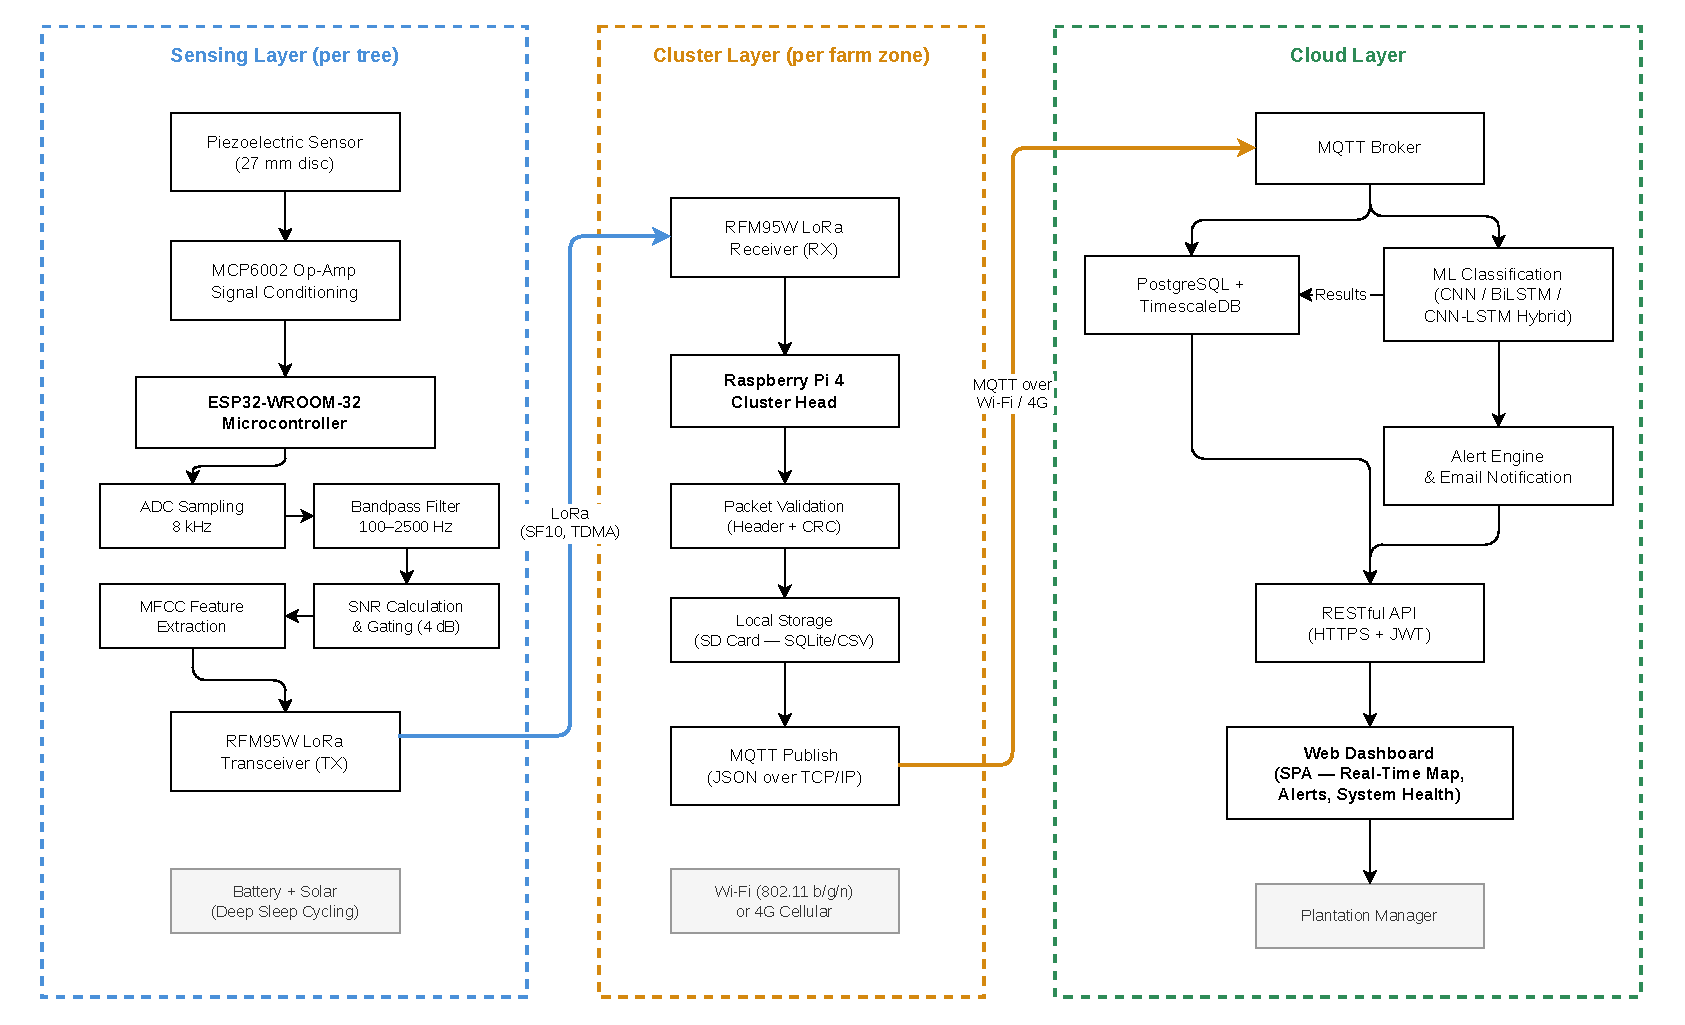
\includegraphics[width=1\textwidth]{figures/system_fig_diagram.pdf}
\caption{High-level block diagram of the proposed RPW acoustic detection system}
\label{fig:HighLevelBlockDiagram}
\end{figure}

\subsection{Sensing Layer}

\newrevision{The communication sender submits a locally produced probability through the result API. The six-byte application record is frozen in a bounded RAM queue and sent using the versioned LoRa protocol. The broader sensor acquisition and mechanical playback proposals remain separate from this communication demonstration.}

\newrevision{The updated feature-packet design uses temporal delta, ZigZag, and predefined coefficient-specific Rice schedules (Section~\ref{sec:codec_design}). Its offline size comparison is reported in Section~\ref{sec:codec_results}. Protocol versioning, embedded resource use, and radio performance remain to be verified.}

\subsection{Cluster Layer}

\newrevision{The cluster head validates and forwards packets using the component and reception logic in Section 4.3.}

\newrevision{Multiple cluster heads are a future deployment option. Geographic zoning alone does not establish interference-free operation or linear scaling; channel reuse, traffic, airtime and simultaneous-node measurements are required before those claims can be made.}


\subsection{Cloud Layer}

\newrevision{The implemented bench receiver validates binary HTTP requests and stores classification-result records in SQLite on a computer. Cloud inference, alerts and dashboard integration described below are proposed services, not functions validated by the historical radio logs.}

\section{Hardware Design}

The hardware architecture of the system is organized into two layers: the sensing node (deployed per tree) and the cluster head (deployed per farm zone), with data ultimately flowing to a cloud backend for classification and monitoring. Below is a detailed description of every component in the system.

\subsection{Piezoelectric Disc Sensor}

\newrevision{Each sensing node uses the WANGCL piezoelectric vibration sensor and an MCP602E conditioning circuit. The sensor is held against the palm surface by a pressing plate. This mounting uses surface contact, without the previously proposed drilled metallic waveguide. Mounting pressure, coupling, and background vibration remain controlled test factors.}


\subsection{MCP602E Op-Amp Signal Conditioning Circuit}

\newrevision{Figure~\ref{fig:sensing_node_schematic} shows the complete supplied sensing-node connections, including the power circuit. The ESP32 receives a 5 V input and supplies the 3.3 V rail used by the sensor, MCP602E, and SX1278.}

\newrevision{The 3.7 V LiPo connects to the TP4056 module's B+ and B- terminals. USB-C provides the charger's 5 V input. The module's OUT+ passes through switch SW1 to the XL6009 boost-converter IN+, while OUT- connects to IN- and the system ground. The XL6009 output is adjusted to 5.0 V and feeds the ESP32 input. All ground symbols represent a common net, and all +3V3 symbols represent the ESP32's 3.3 V rail.}

\newrevision{The marked current-measurement point is on the 5 V line between the boost converter and ESP32. A reading taken there includes the ESP32 and its downstream sensor, conditioning circuit, and radio loads, but excludes boost-converter losses and charger consumption. Battery-side energy and battery life therefore require separate measurements.}

\newrevision{R1 and R2 (100 k$\Omega$ each) divide the 3.3 V supply to a nominal 1.65 V bias, smoothed by C1 (10 $\mu$F). MCP602E channel U1B buffers this bias. The sensor signal passes through C2 (100 nF) and is biased through R3 (100 k$\Omega$); their ideal high-pass corner is approximately $1/(2\pi R_3C_2)=15.9$ Hz. U1A is a voltage follower with gain 1, providing buffering rather than voltage amplification. Its output connects through R4 (1 k$\Omega$) to GPIO34 (ADC1). C3 (100 nF) bypasses the op-amp supply. These are schematic values; measured bias, frequency response, and clipping behavior remain to be documented.}

\newrevision{The SX1278 connections are GPIO18 to SCK, GPIO19 to MISO, GPIO23 to MOSI, GPIO27 to NSS, GPIO14 to RESET, and GPIO26 to DIO0, with a shared ground and a 433 MHz antenna. The analog high-pass corner is separate from the proposed digital 100--2500 Hz bandpass filter.}

\begin{landscape}
\begin{figure}[p]
\centering
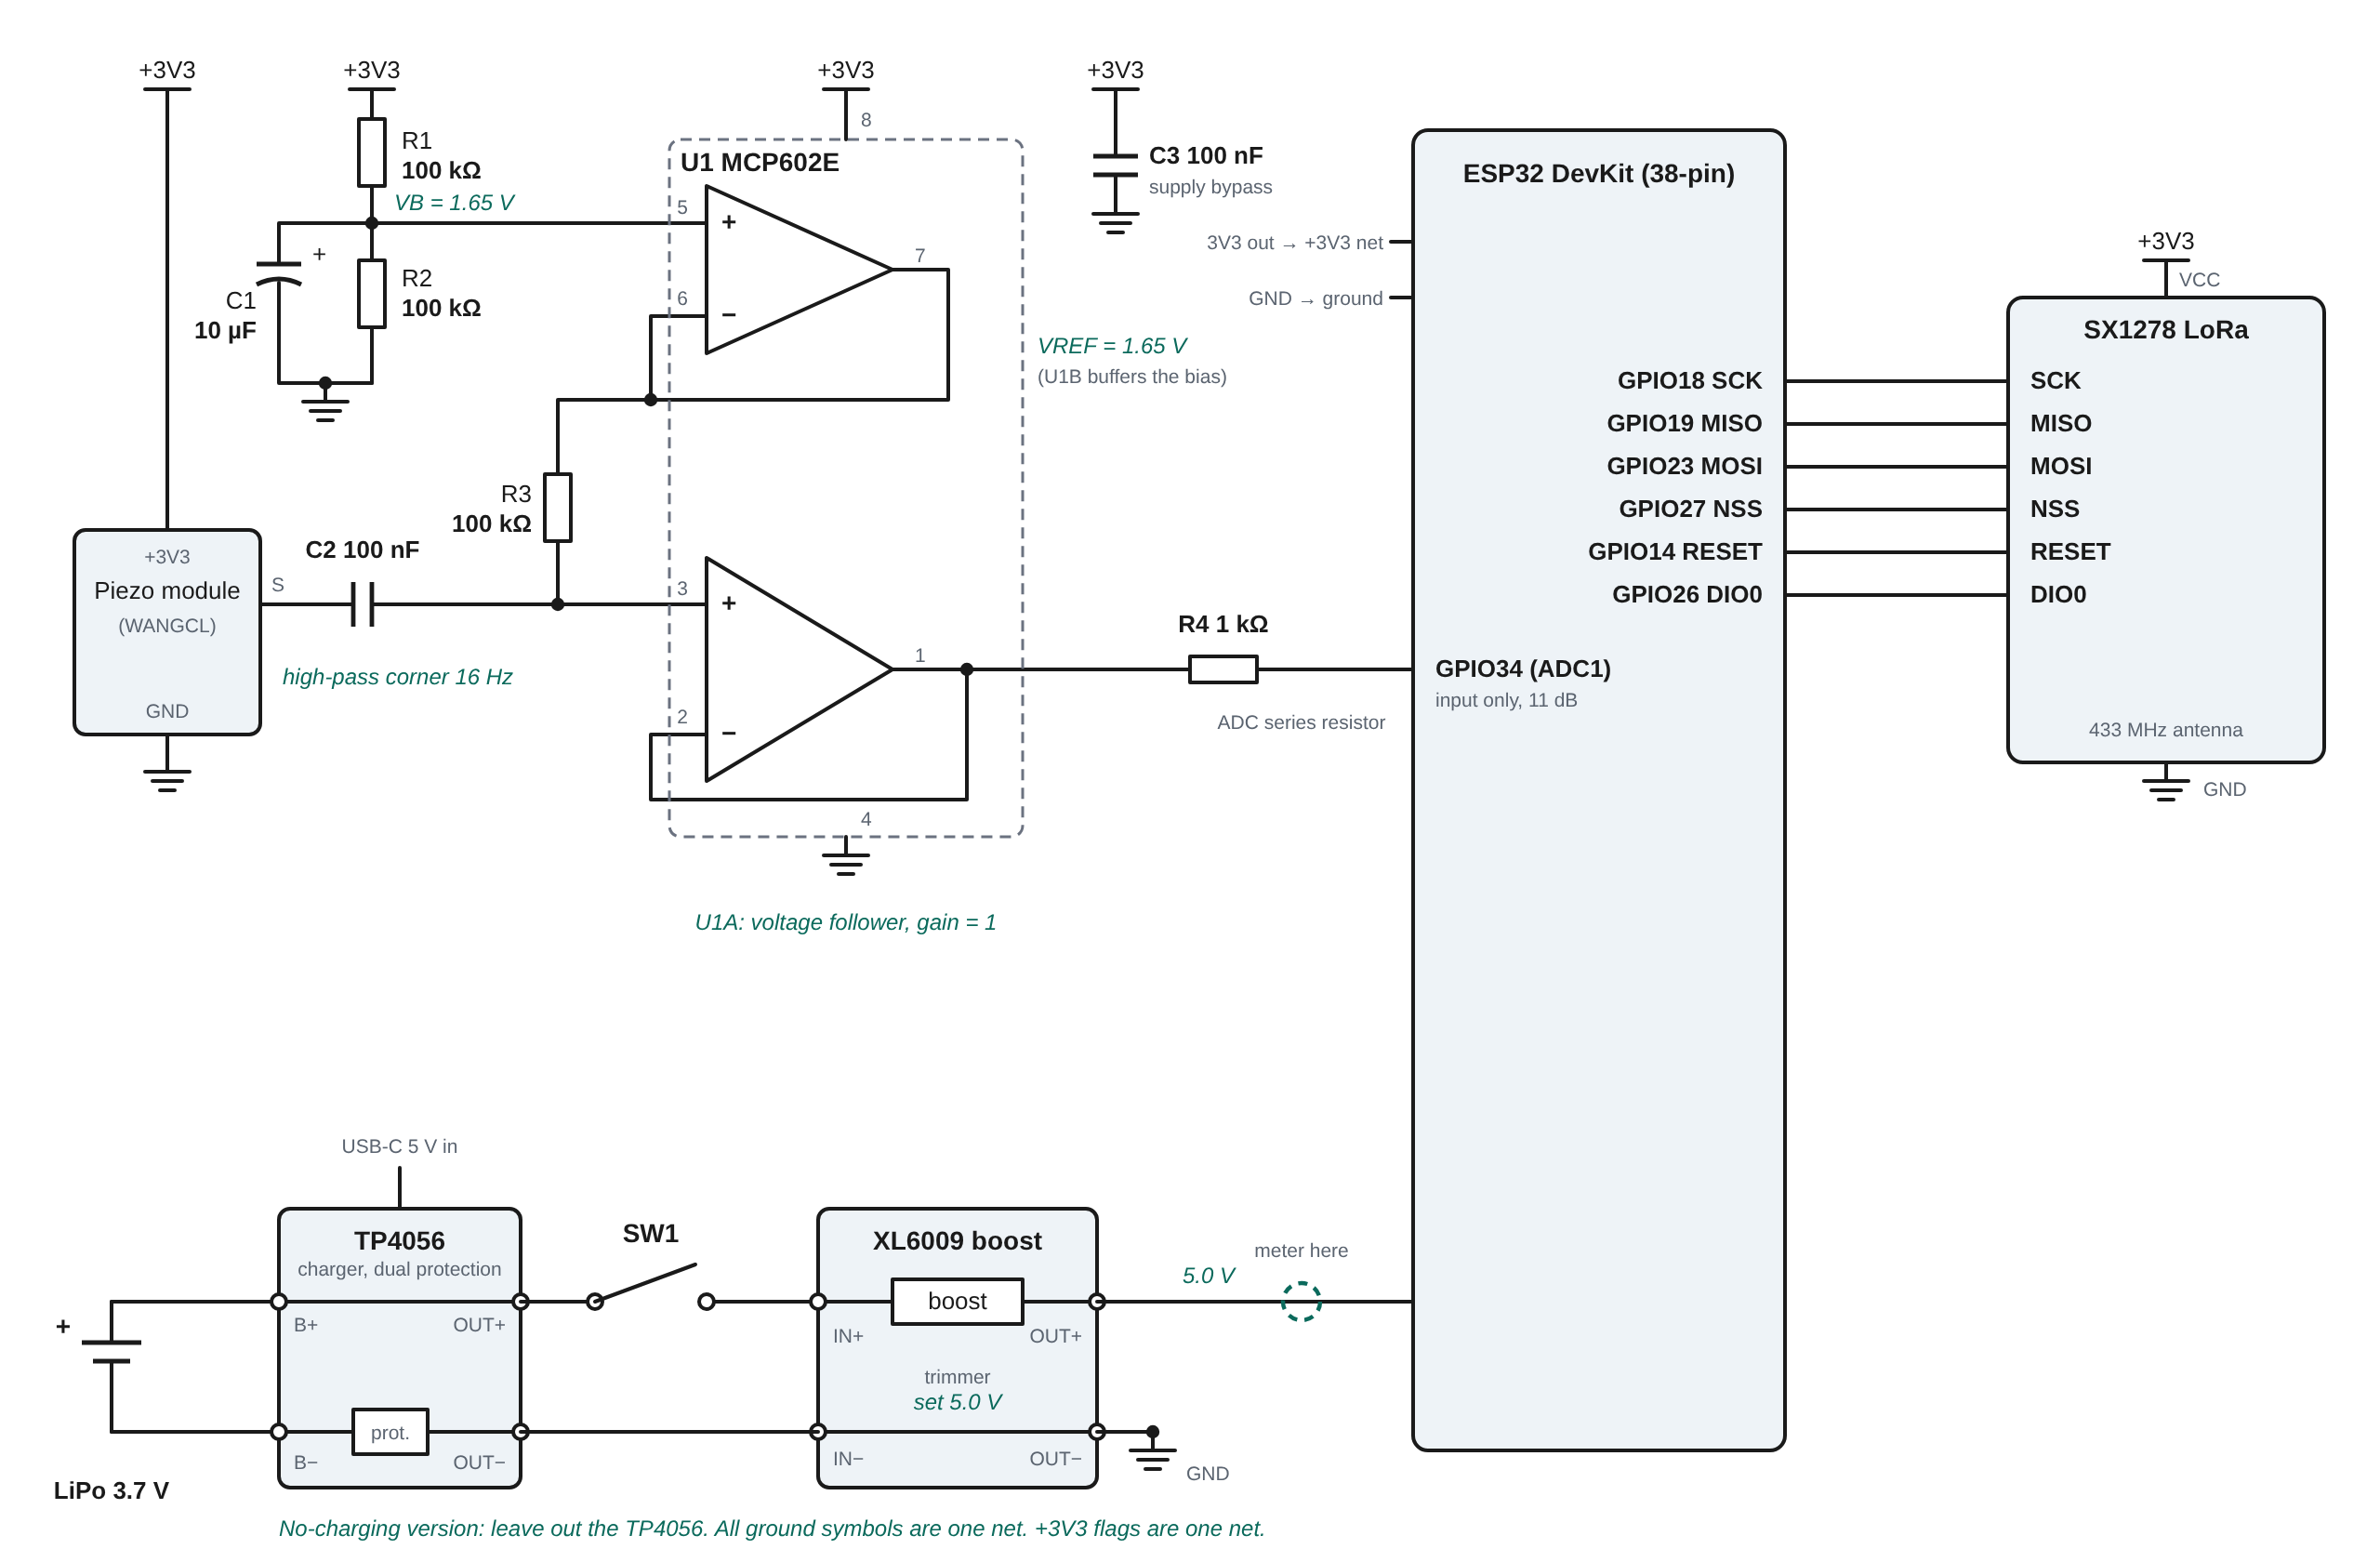
\includegraphics[width=\linewidth,height=0.8\textheight,keepaspectratio]{figures/sensing_node_full_schematic.png}
\caption{\newrevision{Complete team-supplied sensing-node schematic, including LiPo charging, switch, 5 V boost supply, sensor conditioning, ESP32 ADC, and SX1278 connections. The marked meter position is on the boost output supplying the ESP32.}}
\label{fig:sensing_node_schematic}
\end{figure}
\end{landscape}


\subsection{ESP32 Microcontroller}

The ESP32 serves as the brain of the sensing node. It performs ADC sampling and executes the on-node signal processing pipeline described in Section 4.3.3. No raw audio ever leaves the node; the payload will contain either compact MFCC features or a local classification result, selected after model testing. The ESP32 was selected for its low cost, integrated Wi-Fi (useful for bench testing), adequate ADC resolution, and broad community support through the Arduino ecosystem.

\subsection{LoRa Transceivers}

Wireless communication between the sensing node and cluster head uses an SX1278 operating at 433 MHz and connected to the ESP32 through SPI. \newrevision{The communication tests used SF7, 125 kHz bandwidth, coding rate 4/5, and configured TX power of 10 dBm (Section~\ref{sec:communication_results}). Deployment settings remain subject to the applicable local frequency plan.} Range and hourly capacity depend on payload airtime, permitted duty cycle, interference, antenna placement, and plantation conditions; the earlier 1 km and 8,000-transmission values are planning estimates that require measurement. Transmission scheduling and payload composition are described in Section 4.3.3.

\subsection{LoRa Antenna}

\newrevision{The communication prototype uses 433 MHz spring antennas on the SX1278 radios. Antenna orientation, mounting height, and gain have not been documented. Deployment antennas must match the selected frequency plan.}

\subsection{ESP32 Cluster Head}

\newrevision{The cluster head is an ESP32 connected to an SX1278 LoRa receiver over SPI. Its role is to receive packets and forward them to the cloud server over Wi-Fi. The forwarding architecture is confirmed; end-to-end operation and outage recovery will be reported when test results are available.}


\subsection{Casing \& Optional Solar Panel}

\newrevision{Outdoor enclosure protection remains a design target. Solar hardware has not been purchased or evaluated and remains a future option. The implemented battery supply is described in Section~\ref{sec:HardwareImplementation}.}




\section{\newrevision{System Architecture and Software Design}}

This section presents the software design of the RPW acoustic detection system. It covers the overall system architecture, the data architecture underlying persistent storage and data flow, and the detailed design of both static and dynamic system behaviors. Each diagram included in this section is discussed in the accompanying text.



\subsection{System Architecture}

A detailed description of the overall physical architecture of the application is presented in this section.

\subsubsection{Node Architecture}
\newrevision{The implemented communication path uses local inference with classification-result transmission. A separate compressed-MFCC path is retained for comparison; it is not accepted or forwarded by the current result-only head. Descriptions of feature preprocessing, cloud inference and production dashboard services below are design proposals rather than demonstrated behavior of the bench transport.}


The IoT-based RPW acoustic detection system is organized into a three-tier physical architecture comprising (1) the sensing node layer, (2) the cluster head aggregation layer, and (3) the cloud backend and dashboard layer. Each tier has clearly defined responsibilities and communicates with adjacent tiers through well-specified interfaces, enabling modular development, independent scaling, and fault isolation across the deployed network.

\paragraph{Sensing Node Layer} 

\newrevision{The deployment sensing node uses the hardware in Section 4.2. For the implemented communication demonstration, the application submits a valid local inference probability; the radio sends six application bytes inside the 34-byte packet, following beacon admission and assigned TDMA cells. No raw audio, feature matrix, acoustic SNR gate or full recording timestamp is added by the communication layer. The earlier sensing proposal includes filtering, SNR gating, MFCC extraction and scheduled sleep; these remain separate acquisition/deployment work. Its former 900 ms slot assumption is superseded for this demo by the 1,099 ms per-node slot in Section~\ref{sec:communication_protocol}.}

\paragraph{Cluster Head Aggregation Layer}

\newrevision{The intermediate tier uses an ESP32/SX1278 head. It validates protocol fields and CRC, rejects invalid/conflicting records and queues accepted result packets before radio ACK. A separate Wi-Fi task forwards the original binary packet by HTTP. This separation avoids intentionally blocking radio service on network requests; queueing and restart limits are specified in Section~\ref{sec:communication_protocol}.}


\paragraph{Cloud Backend and Dashboard Layer}

\newrevision{The current receiving computer runs a Python standard-library HTTP service and SQLite database. A later cloud/dashboard deployment may add Linux services, feature inference, time-series storage, alerts and authenticated APIs. These are integration targets, not the implemented bench receiver. The existing result path does not use an MQTT broker or forward MFCCs for cloud classification.}

\subsubsection{Node Topology}

\newrevision{The implemented topology is one sensing sender communicating directly with one head over LoRa, followed by Wi-Fi to a receiving computer. Two radio slots are reserved by the protocol, but multi-node and multi-head scalability remain unvalidated. The proposed deployment may extend this arrangement to multiple heads, subject to measured coverage, interference, capacity and power budgets. This is direct LoRa, not LoRaWAN; no mesh or multi-hop routing is implemented. Figure~\ref{fig:ThreeTierNodeArchitecture} shows the updated sensing-node, cluster-head and receiving-computer communication path; the packet and delivery specification is given in Section~\ref{sec:communication_protocol}.}


\begin{figure}[h]
\centering
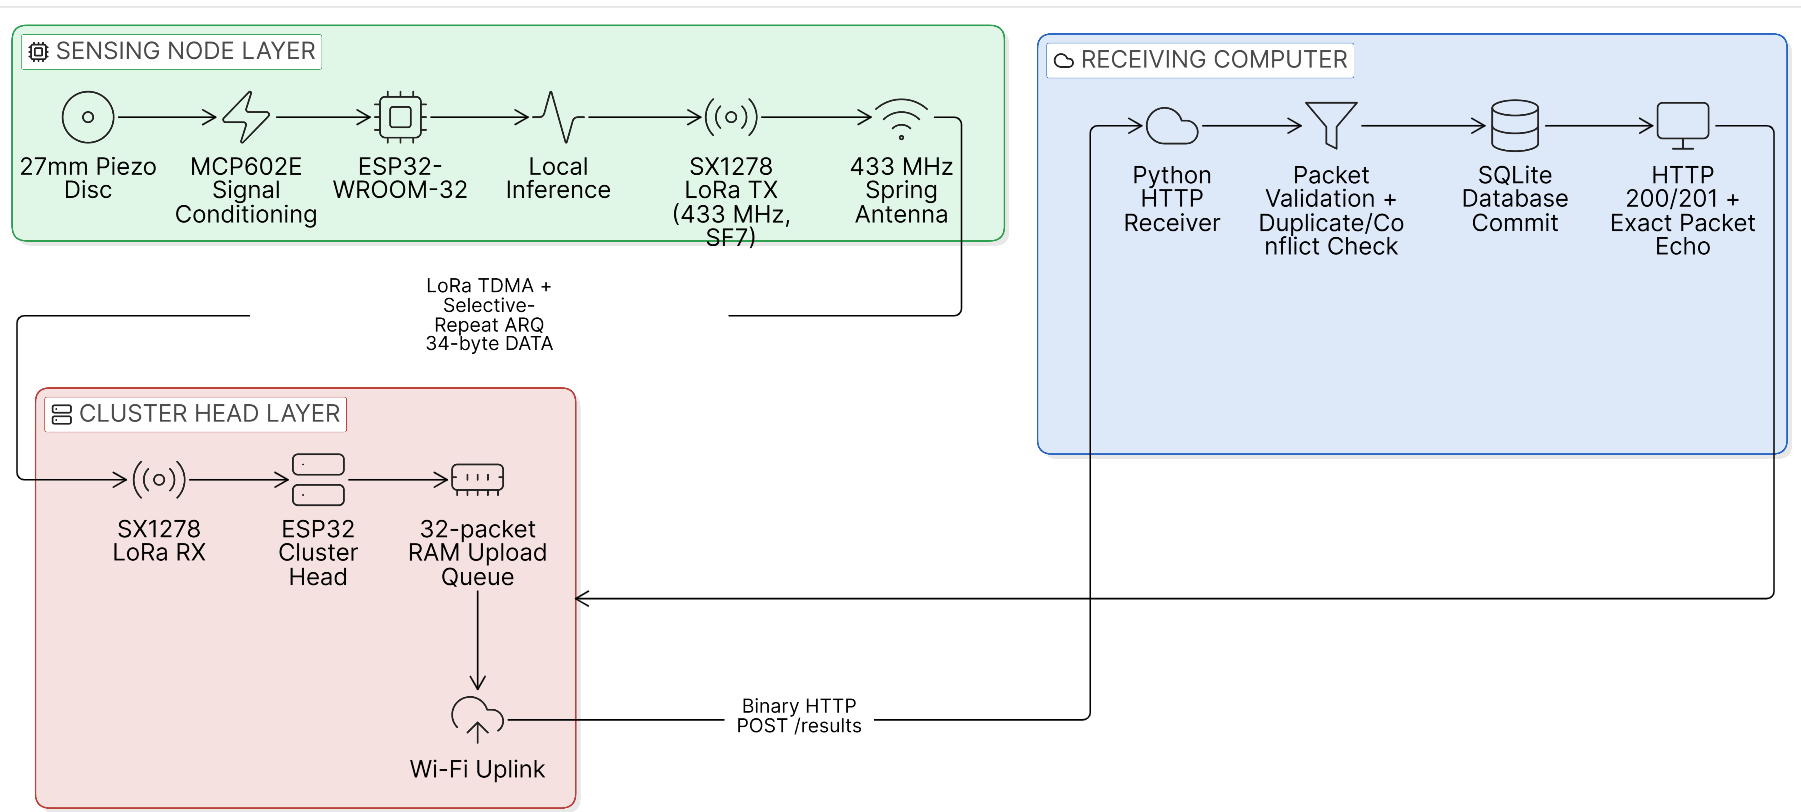
\includegraphics[width=0.95\textwidth]{figures/3Node_Arch.png}
\caption{Three-Tier Node Architecture of the IoT-Based RPW Acoustic Detection System}
\label{fig:ThreeTierNodeArchitecture}
\end{figure}


\subsubsection{Component Architecture}

Each tier of the system is composed of several internal software components that handle distinct stages of the detection pipeline. This section describes the responsibilities of each component and how they are organized within their respective nodes.

\paragraph{Sensing Node}

\newrevision{The communication API queues immutable application records and tracks queued, in-flight, acknowledged or unconfirmed status. The sender follows beacon admission, its assigned slot and selective-repeat ACK masks. Sleep scheduling, live battery acquisition and acoustic triggering are not provided by this communication layer. Bench day is manually set and battery is simulated; the three-bit battery field is not a separate low-battery flag or calibrated voltage measurement.}

\paragraph{Cluster Head}

\newrevision{The head validates packets and queues complete accepted DATA in a 32-entry volatile RAM FIFO before acknowledging new records. Its duplicate history covers 256 events in addition to active-batch checks. A full/unavailable queue leaves new records unacknowledged. Pending uploads are retried over Wi-Fi, but a head restart loses them. SQLite persistence is on the receiving computer, not the ESP32.}


\paragraph{Cloud Backend}

\newrevision{The bench receiving service accepts \texttt{POST /results} with exactly 34 binary bytes, validates them and commits a SQLite row before returning success. Its event identity is node ID, sender boot token and measurement ID. Matching duplicates return success without another event; different application bytes under the same identity return a conflict. Later cloud preprocessing, inference, alert and dashboard services remain proposed and do not change the bench delivery contract.}

\subsubsection{Class Architecture and Static Representation}

The class architecture consists of 4 classes: ClusterHead, SensingNode, SensorMeasurement, and Tree. The ClusterHead and SensingNode classes represent the hardware components of Cluster Head and Sensing Node. Each ClusterHead can have many Sensing nodes connected to it, and each SensingNode can be connected to one ClusterHead. This relationship is represented by a bidirectional aggregation association relationship.


\begin{figure}[h]
\centering
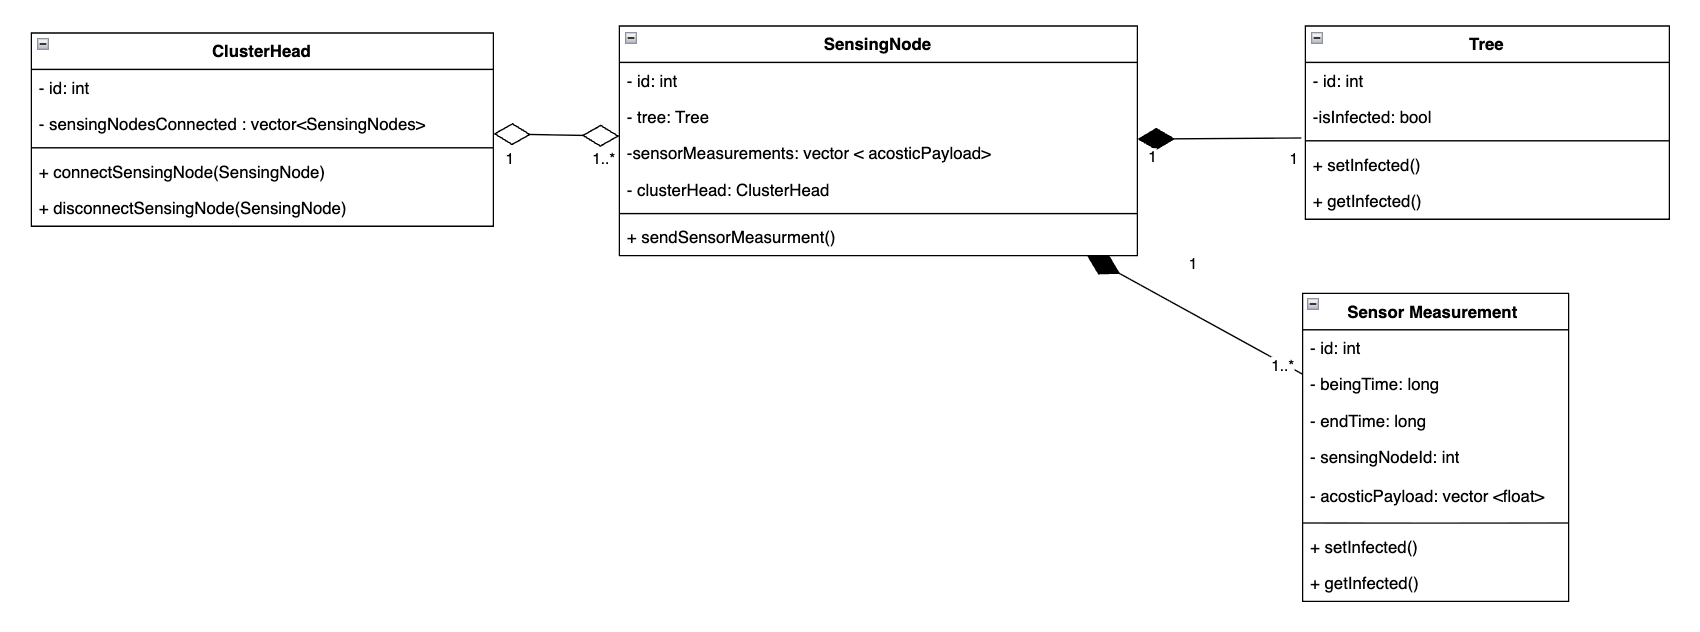
\includegraphics[width=1\textwidth,height=1\textheight,keepaspectratio]{uploads/Class Daigram.png}
\caption{Class architecture diagram of the RPW detection system}
\label{fig:ClassArchitectureDiagram}
\end{figure}

The SensorMeasurement class represents one “Chunk” of acoustic measurements, with a start time stamp, end time stamp, and an acoustic payload. Each SensingNode can have many SensorMeasurement stored in a dynamic array (vector). Each SensorMeasurement can only belong to one SensingNode. This is represented by a 1 to many composition relationship, because without a SensingNode no SensorMeasurement can be made. Each SensingNode is also associated with one tree, and each tree is associated with one sensing node, this relationship is represented by a one-to-one composition association, because without a SensingNode we cannot monitor a tree, and therefore for a tree to exist in our system it must be associated with exactly one sensing node.

\subsection{Data Architecture}

\newrevision{The following production database schema is a proposed integration target, not the current bench SQLite schema. The six-byte radio result carries no MFCC matrix, battery millivolts, uptime or complete source timestamp. The bench receiver stores server ingestion time, which must not be described as recording time; health fields require separate telemetry and calibration.}

The data architecture is built on PostgreSQL extended with TimescaleDB. PostgreSQL provides a relational database engine supporting complex queries via standard SQL, while TimescaleDB adds automatic time-based partitioning (hypertables) and range-query performance suited to the continuous timestamped MFCC feature streams produced by the sensing layer. Together, they manage all relational data, cluster head and node metadata, time-series acoustic features, classification results, and user accounts, within a single database instance. The database schema consists of seven tables distributed across the three system layers. Figure 4.4 presents the ER diagram of the complete schema.

\begin{figure}[h]
\centering
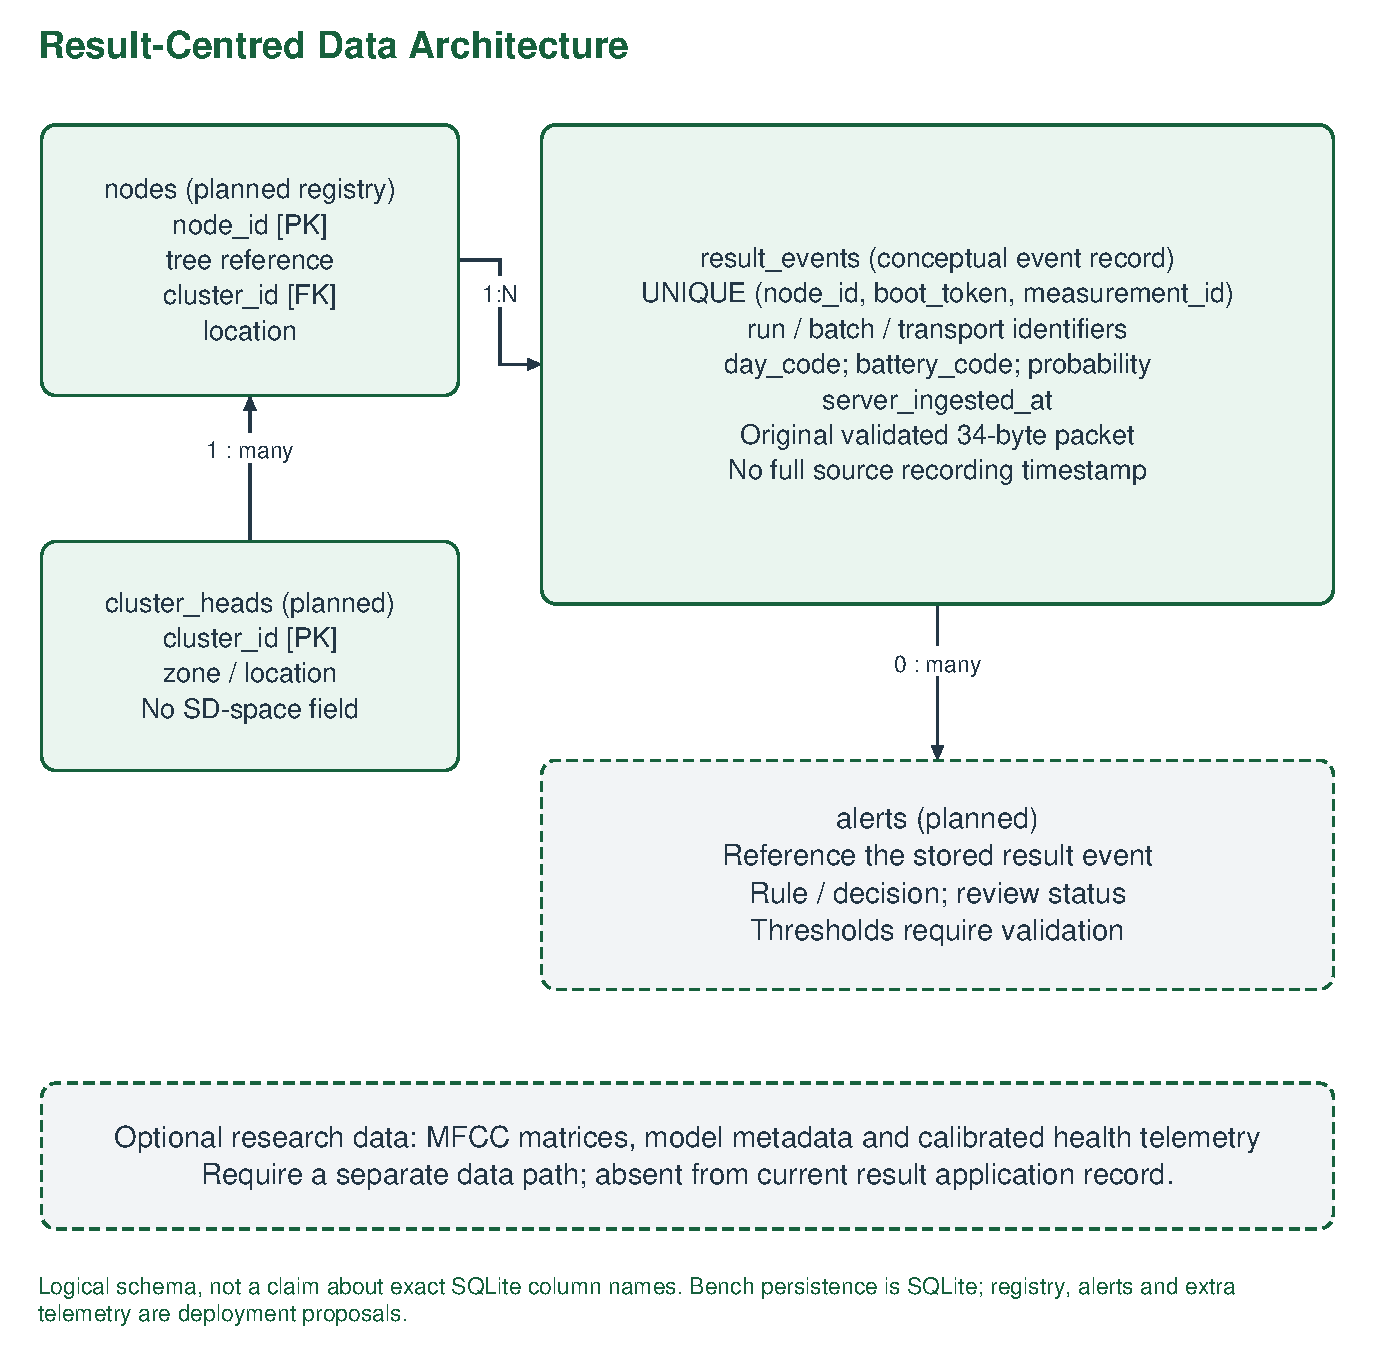
\includegraphics[width=0.95\textwidth]{figures/ER_Diagram.pdf}
\caption{Entity-Relationship diagram of the RPW detection system database}
\label{fig:EntityRelationshipDiagram}
\end{figure}

\subsubsection{Sensing Layer Tables}

The nodes table stores the registration record for each deployed sensing node, identified by a node id primary key (varchar). Each row contains the associated cluster id foreign key, the farm zone designation, geographic coordinates (location lat, location lon), and install date.



The relationship to cluster heads is one-to-many: each cluster head may have many sensing nodes, but each node belongs to exactly one cluster head. The node health hypertable records periodic health telemetry from each sensing node, indexed by a composite key of timestamp (timestamptz) and node id. Data columns include battery mv (millivolts), rssi dbm (dBm), and uptime s (seconds since last reset). Time-based partitioning keeps range queries efficient as the table accumulates months of deployment data. The acoustic features hypertable stores the preprocessed feature data transmitted by sensing nodes, indexed by timestamp and node id. The primary data column is mfcc (a 15×13 int8-quantized representation of the extracted MFCC vector), accompanied by snr db. Since feature extraction occurs entirely on the sensing node, no raw audio is stored. Records are retained for one year to support longitudinal infestation trend analysis.

\subsubsection{Cluster Layer Tables}

\newrevision{The planned cluster-head records contain identifiers, farm zone, location, installation date, and Wi-Fi uplink status. Health telemetry will cover uptime, RSSI, and connectivity. SD-card free-space fields in the earlier schema and diagram are obsolete and require removal during schema implementation.}


\subsubsection{Cloud Layer Tables}

The classification results hypertable stores the output of the deep learning inference pipeline, indexed by timestamp and node id. Each row contains the predicted label (e.g., ``infested'' or ``healthy''), the confidence score (0.0--1.0), and the model version identifier. Storing the model version with each result supports performance comparisons across model updates. The alert log hypertable records all detection alerts, indexed by timestamp and node id. Each row contains the alert type (e.g., ``infestation detected''), the classification confidence that triggered the alert, and an acknowledged flag indicating whether a plantation manager has reviewed it. Alert logs, along with the nodes and cluster heads metadata tables, are retained indefinitely.

\subsubsection{Data Retention and Partitioning Strategy}

The four hypertables are automatically partitioned by TimescaleDB along the timestamp dimension. Time-range queries, for example, retrieve all classification results for a specific farm zone over the past 30 days, executed against only the relevant partitions rather than the full table. Acoustic features and classification results are retained for one year, after which aged-out partitions are dropped automatically.

\subsection{Detailed Design}

\subsubsection{Dynamic Representation}

\newrevision{The existing sensing and cluster flowcharts are retained as earlier conceptual designs. They do not describe the current result-only communication implementation. The text below and Section~\ref{sec:communication_protocol} specify the implemented transport; acquisition and offline feature processing remain separate.}

\newrevision{Figure~\ref{fig:SensingLayerFlowchart} retains the earlier sensing proposal, while Figure~\ref{fig:ClusterLayerFlowchart} retains the earlier cluster design. Their older radio, storage and forwarding assumptions are not implemented communication claims. The following text separates current result submission, radio acceptance and computer persistence.}

\paragraph{Sensing Layer Operational Flow}

\begin{figure}[H]
\centering
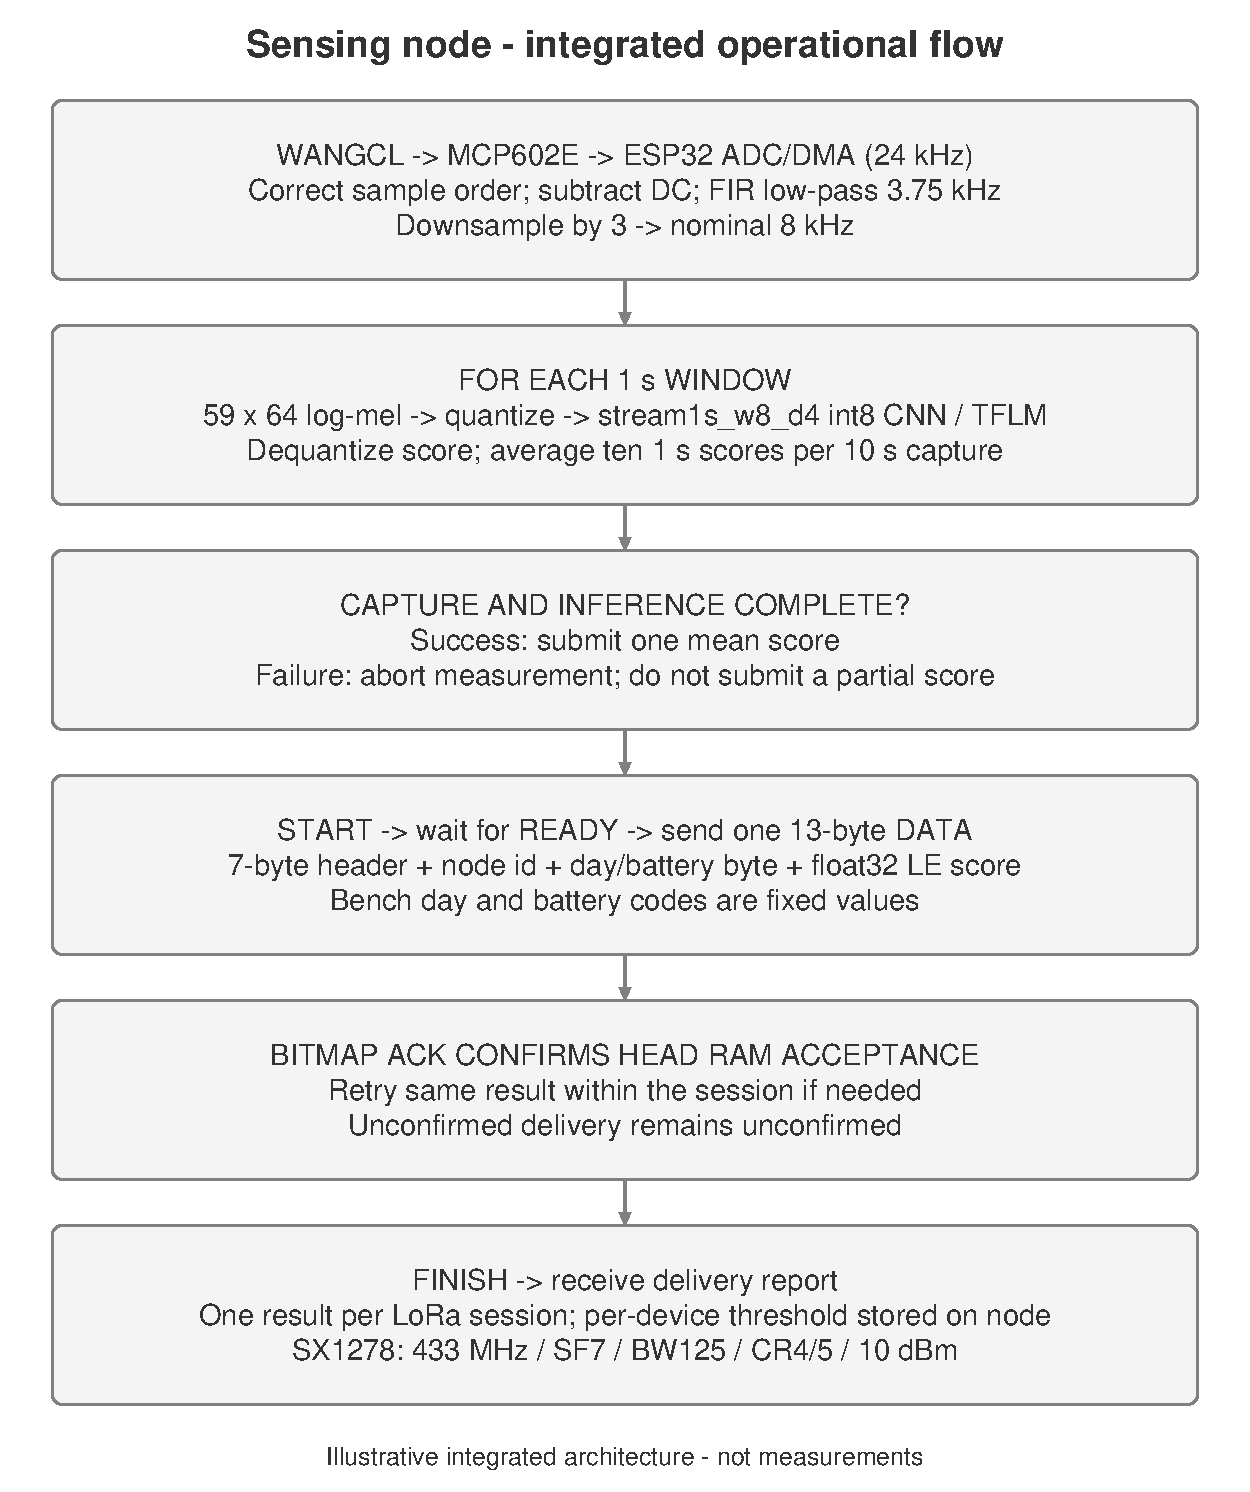
\includegraphics[width=0.88\textwidth,height=0.72\textheight,keepaspectratio]{figures/Sensing_layer_flowchart.pdf}
\caption{Sensing Layer operational flowchart}
\label{fig:SensingLayerFlowchart}
\vspace{0.5\baselineskip}
\end{figure}
\FloatBarrier

\newrevision{The implemented sender path begins when the application submits a valid probability. It does not assert live sampling, SNR gating or MFCC transmission. The queued application bytes retain the original result throughout retries. The sender waits for the head beacon and admission, then uses its DATA cells and the cumulative ACK bitmap; unconfirmed results are reported when bounded recovery ends.}

\newrevision{The earlier SNR-gated acquisition design is distinct from this communication path. Its 214-byte/approximately 440 ms MFCC transmission remains an assumption in the retained flowchart, not a measured property of the current result demo. Compressed-feature sizes are variable and need their own complete packet definition and airtime calculation; the offline comparison remains in Section~\ref{sec:codec_results}.}

\paragraph{Cluster Layer Operational Flow}

\begin{figure}[H]
\centering
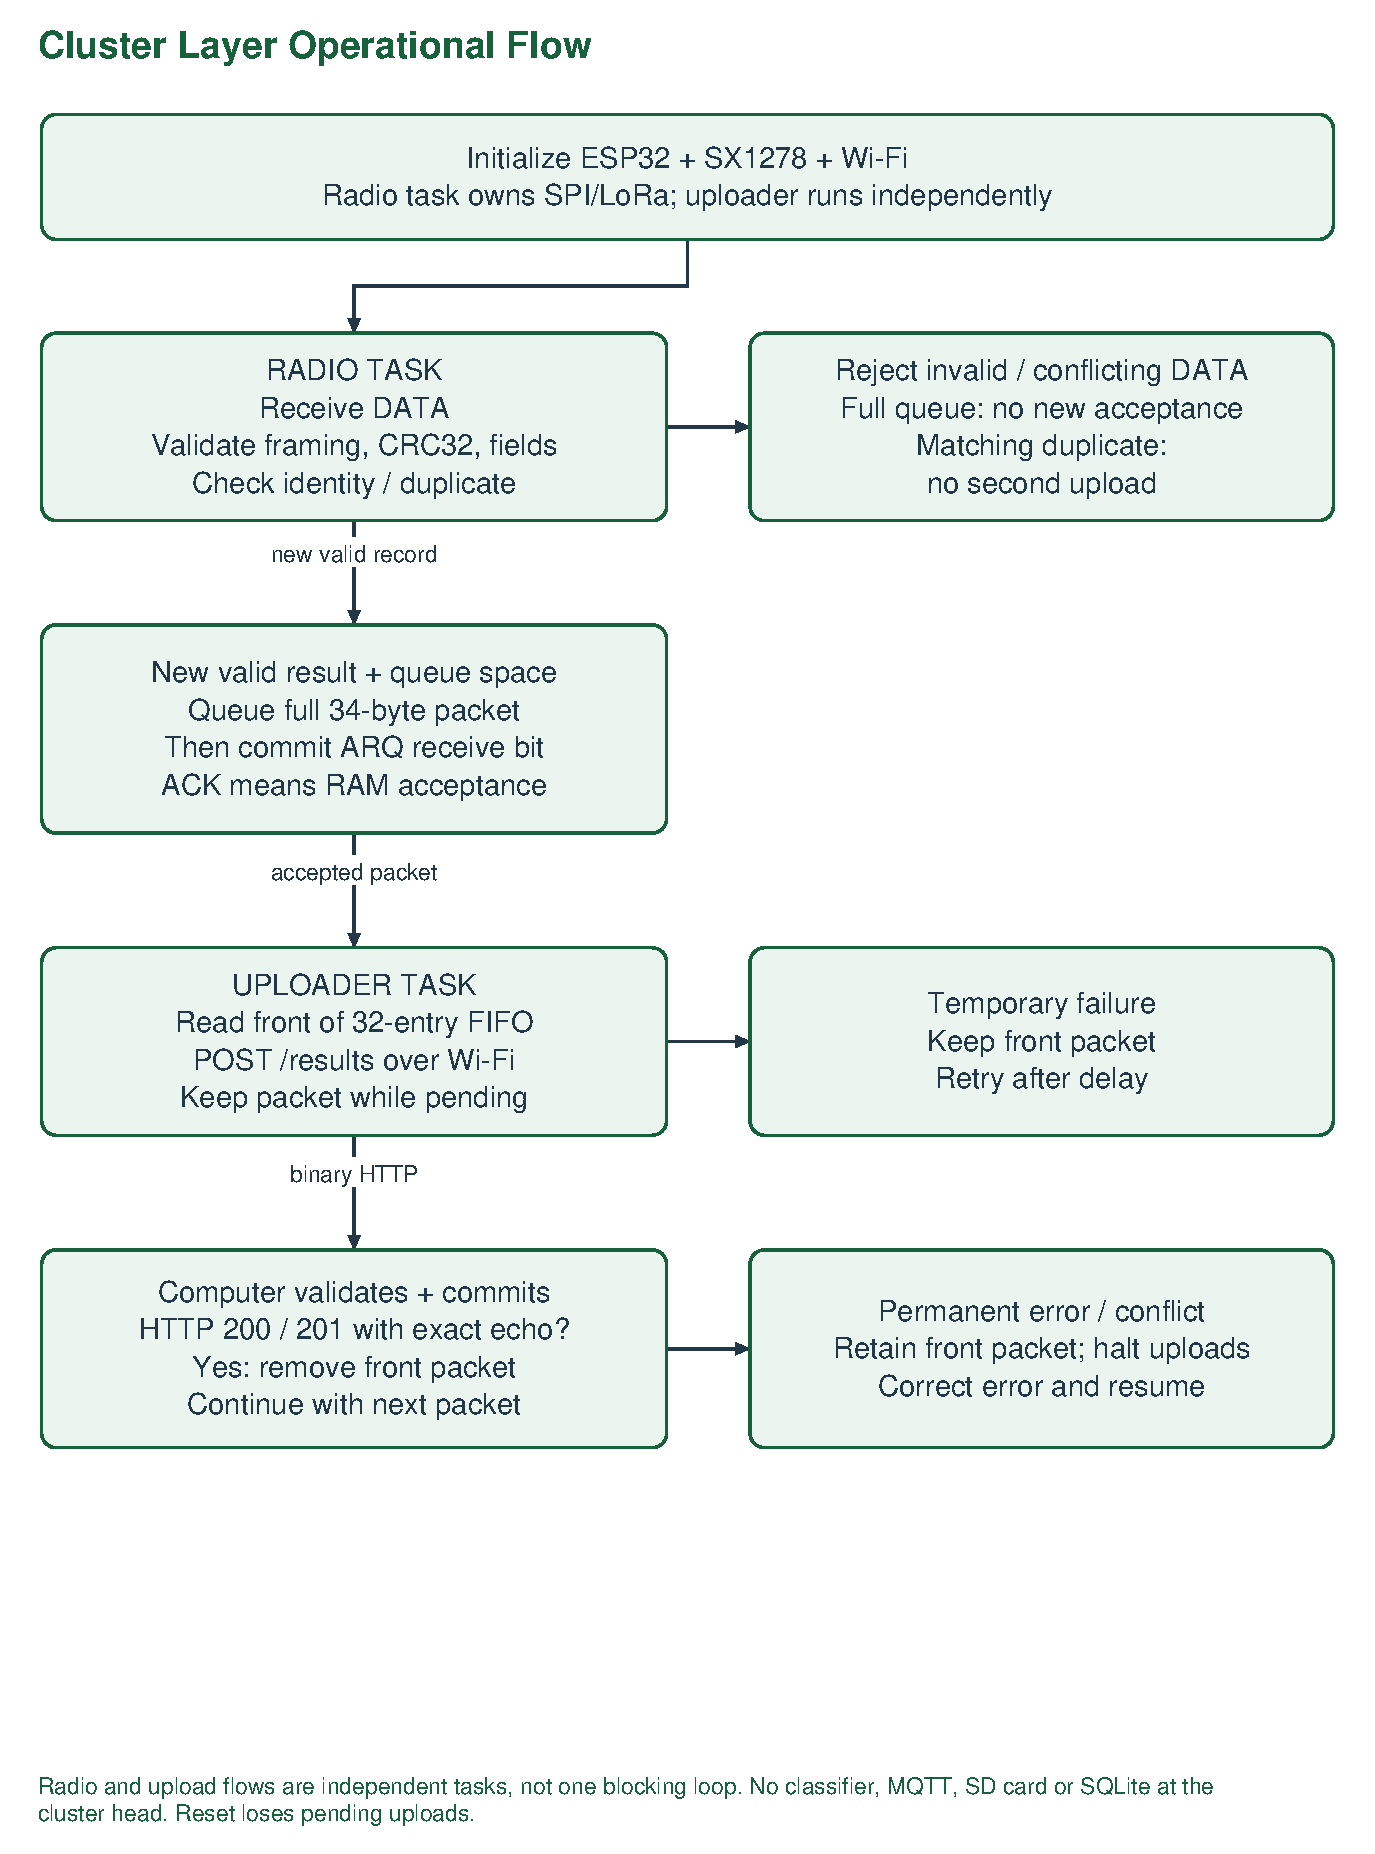
\includegraphics[width=0.88\textwidth,height=0.72\textheight,keepaspectratio]{figures/Cluster_layer_flowchart.pdf}
\caption{Cluster Layer operational flowchart}
\label{fig:ClusterLayerFlowchart}
\vspace{0.5\baselineskip}
\end{figure}
\FloatBarrier

\newrevision{The head initializes the ESP32/SX1278 radio and Wi-Fi uploader. Radio and upload work are separate tasks; only the radio task owns SPI/LoRa. On reception, the head checks framing, CRC and application fields before accepting a new result.}


\newrevision{A new valid result is queued before its ARQ receive bit is committed. Matching repeated records do not create another upload; invalid records or identity conflicts are rejected. A radio ACK confirms head RAM acceptance, not computer persistence.}


\newrevision{The uploader retains its front packet until HTTP 200/201 and an exact echo confirm the receiving service has committed it or recognized a matching stored event. Temporary network/server failures cause delayed retries. Permanent errors retain the front packet and halt uploads until corrected and resumed.}


\newrevision{The head carries no classifier but is not stateless: upload queues, admission state and duplicate history are held in bounded volatile RAM. There is no SD card, SQLite database, persistent head outbox or replay after head reset. No supported plantation-wide node count is claimed from this one-pair demonstration.}

\subsubsection{\newrevision{Earlier Version-5 Communication Demonstration}}
\label{sec:communication_protocol}
\begingroup
\color{green!45!black}
This demonstration used version-5 framing between the sender and the cluster head. The integrated system test used the single-result link in Section~\ref{sec:integrated_result_link}. Section~\ref{sec:communication_results} reports the separate eight-byte synthetic radio experiment, and Section~\ref{sec:codec_design} describes the standalone MFCC codec.

\paragraph{Application record and transport packet}
The six application bytes contain node ID (one byte), packed day/battery (one byte), and an IEEE 754 binary32 probability (four little-endian bytes). Bits 7--3 hold day 1--31; bits 2--0 hold battery code 0--7. The percentage encoder uses $\lfloor 7P/100+0.5\rfloor$ after clamping $P$ to 0--100; the public submission API rejects non-finite or out-of-range inputs. The bench day is manually configured and the battery is simulated (100\%, code 7), not measured telemetry. No application reserved bits remain. The packet contains neither a full recording timestamp nor acoustic SNR or MFCCs.

\begin{table}[htbp]
\centering\small\color{green!45!black}
\caption{\newrevision{Version-5 demonstration DATA format before radio physical-layer overhead.}}
\label{tab:current_result_packet}
\begin{tabular}{p{0.16\linewidth}p{0.72\linewidth}}
\toprule
Offsets & Contents \\
\midrule
0--3 & Magic 0xA7, version 5, DATA type 3, transport node ID \\
4--7 & Head/session run ID, uint32 little-endian \\
8--11 & Sender boot token, uint32 little-endian \\
12--15 & Batch ID, uint32 little-endian \\
16--19 & Measurement ID, uint32 little-endian \\
20--23 & Index, count, attempt, application length (6) \\
24--25 & Application node ID; packed five-bit day/three-bit battery \\
26--29 & Probability, float32 little-endian \\
30--33 & CRC32 of bytes 0--29, little-endian \\
\bottomrule
\end{tabular}
\end{table}
The 24-byte transport header, six application bytes and four CRC32 bytes total 34 software DATA bytes. The node IDs in transport and application must match. Session, boot, batch and measurement identifiers support admission, ACK matching and duplicate/conflict handling; they are not security credentials. The LoRa preamble, explicit header, coding and PHY CRC add on-air overhead. At the configured SF7/BW125/CR4/5, eight-symbol preamble and PHY CRC, calculated 34-byte DATA airtime is 77.056 ms (rounded to 78 ms for scheduling). Old 35-byte DATA occupies the same symbol-count step, so removing one byte does not reduce this airtime.
\FloatBarrier

\paragraph{TDMA admission and selective-repeat ARQ}
The head sends a beacon that establishes the timing reference and advertises admitted batches. An unadmitted sender sends READY in its control cell, waits for a later beacon grant, then uses its assigned DATA cells. There is no separate READY\_ACK packet type in this protocol. A node slot contains one control cell, eight possible DATA cells and a dedicated bitmap-ACK opportunity. Each DATA cell is $78+30=108$ ms. The reserved slot is $9(108)+30+67+30=1{,}099$ ms, where 67 ms is rounded 29-byte ACK airtime. Two slots and the scheduler's margins give $60+2(1{,}099)=2{,}258$ ms; beacon airtime is additional to the repeating cycle. The demo builds sender ID 1 and head ID 0; reserved node-2 timing is not evidence of a tested second sender.

Each batch contains one to eight records. A receive bitmap marks accepted records; only unconfirmed positions are retransmitted in their original cells, with already-confirmed cells left silent. Attempts 0--4 give at most five total DATA attempts. A separate 120 s batch timeout bounds stalled work; it is not the usual completion time. A lost ACK can cause an exact duplicate, and terminal sender failure means unconfirmed rather than proof of non-reception. Results are not retained indefinitely after bounded recovery. Multi-node capacity and scheduling stability require physical validation.

\paragraph{Head acceptance, HTTP and persistence}
The head validates packet framing, CRC and application fields. It queues a new complete 34-byte packet in a 32-entry volatile RAM FIFO before committing ARQ acceptance. A full/unavailable queue leaves new records unacknowledged. Bounded duplicate history covers 256 events plus active-batch checks. Matching identities and unchanged application bytes are repeats; conflicting bytes are rejected.

An independent Wi-Fi task sends the same bytes with \texttt{POST /results}, \texttt{Content-Type: application/octet-stream}. The Python receiver validates them and commits a SQLite row before responding with HTTP 201 for a new event or 200 for a matching existing event, echoing the submitted packet exactly. The unique event identity is (node ID, sender boot token, measurement ID). Changed application data under an existing identity returns 409. The head removes a pending packet only after success and an exact echo; temporary failures cause delayed retries, while permanent errors halt uploads with the front packet retained until corrected and resumed.

A LoRa ACK therefore means head RAM acceptance, not computer persistence. Head reset loses pending uploads; no persistent outbox or reboot replay is implemented. UTC ingestion time is computer storage time, not the source recording time. Plain HTTP is restricted to a trusted local network; encryption/authentication remain deployment requirements. Direct LoRa is not LoRaWAN. These are source-level implementation facts and calculations, not new physical delivery, range or latency measurements.
\endgroup
\FloatBarrier


\subsubsection{\newrevision{Alternative MFCC Compression and Feature-Packet Design}}
\label{sec:codec_design}
\begingroup
\color{green!45!black}
The selected architecture sends local classification results. The following codec remains a separate feature-transmission investigation and is not used by the current result-only head. The standalone \texttt{sensing/} firmware implements temporal delta, ZigZag, and coefficient-specific Rice coding for a $15\times13$ signed-int8 MFCC matrix. The codec preserves the quantized matrix and its float32 scale exactly after lossy quantization. Section~\ref{sec:codec_results} reports the host verification results.

\paragraph{Offline feature preparation}
The offline pipeline takes seconds 5--15 from recordings at least 20 s long and uses a centered 10 s clip for recordings between 10 and 20 s. Clips of 10 s or less retain their full duration. The pipeline resamples to 8 kHz and applies a zero-phase 100--2500 Hz bandpass without SNR gating or signal squaring. MFCC analysis uses 25 ms windows, 10 ms hops, a 256-point FFT, 26 Slaney Mel filters, and temporal aggregation into 15 bins with 13 coefficients each. Each recording stores 195 symmetrically quantized int8 coefficients and one float32 reconstruction scale.

\begin{figure}[htbp]
\centering
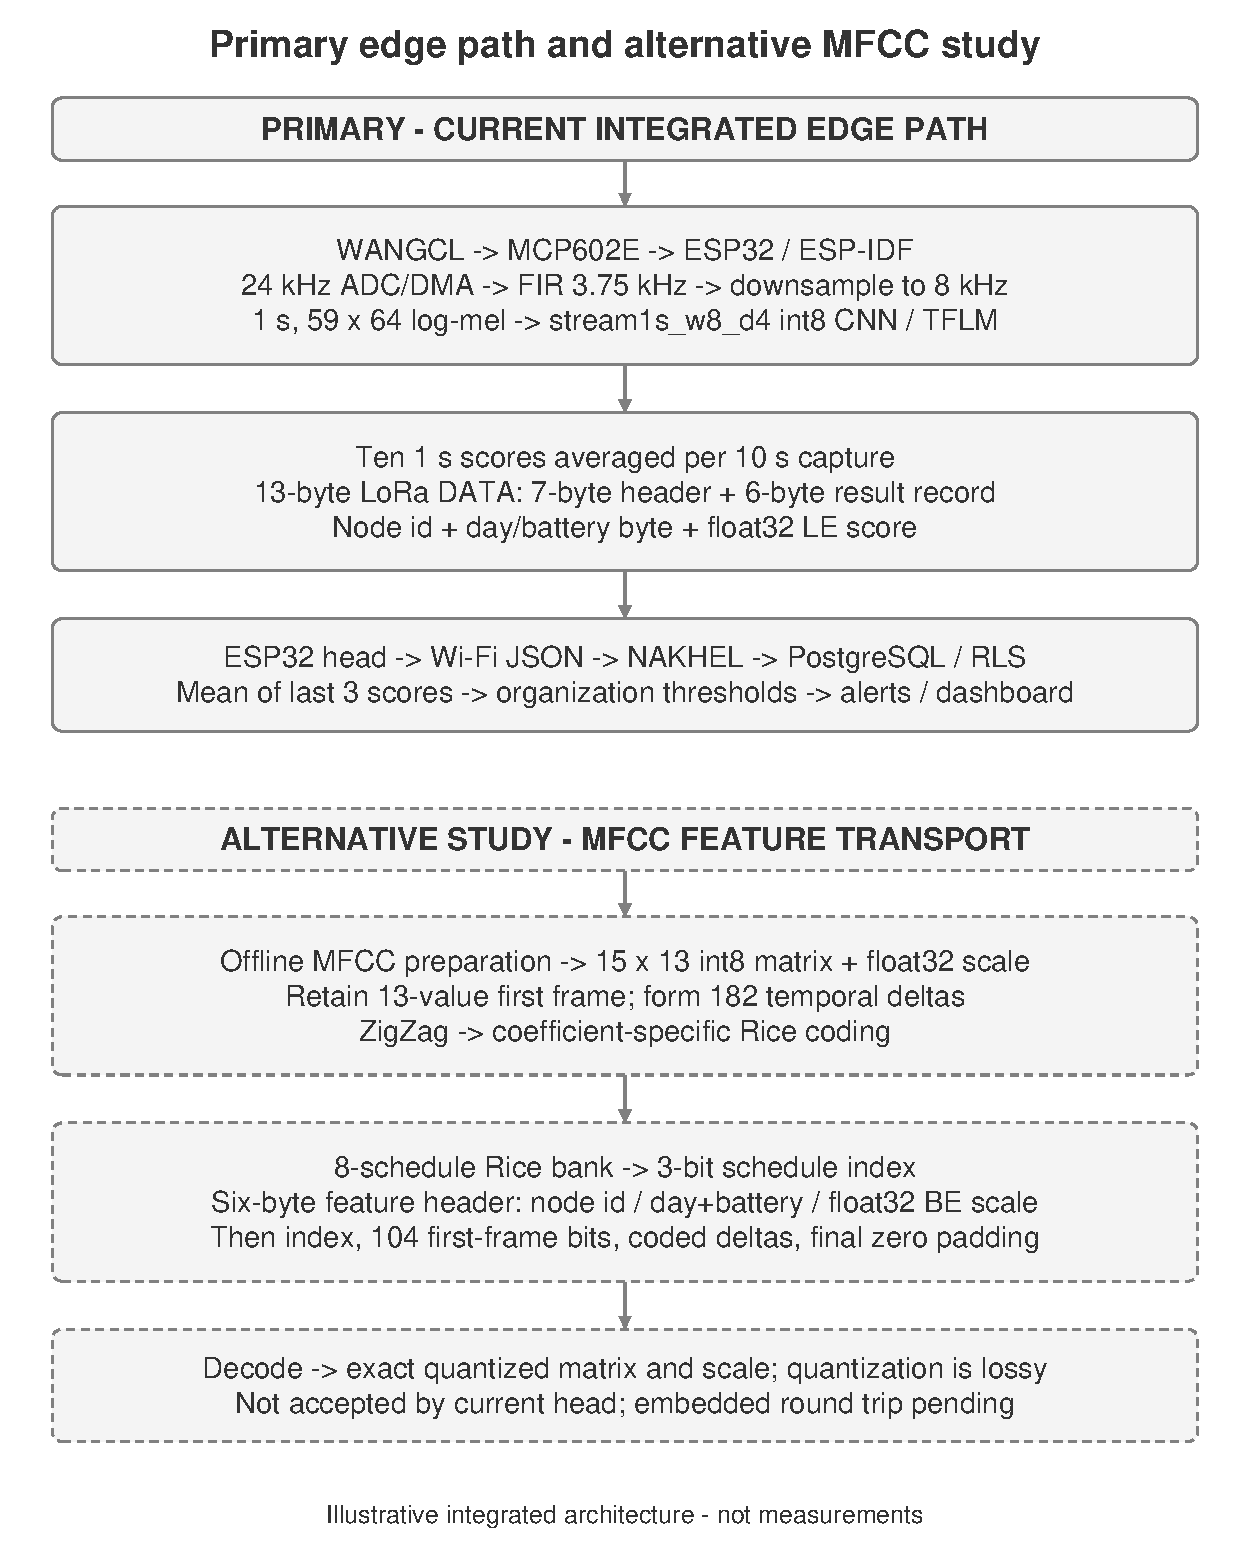
\includegraphics[width=\textwidth,height=0.78\textheight,keepaspectratio]{figures/codec_current_pipeline.pdf}
\caption{\newrevision{Selected edge-inference path alongside the alternative MFCC codec. Feature decoding is separate from the current result-forwarding protocol; exact reconstruction applies only after quantization.}}
\label{fig:codec_current_pipeline}
\end{figure}
\FloatBarrier

\paragraph{Encoding and reconstruction}
The first frame is retained as 13 raw int8 values (104 bits). For each later frame, the encoder computes
\[
d_{t,c}=\operatorname{int16}(Q_{t,c})-\operatorname{int16}(Q_{t-1,c}),\qquad
 t=1,\ldots,14,\quad c=0,\ldots,12.
\]
The 182 differences are between consecutive times within the same coefficient, serialized frame-major. Int16 intermediates accommodate the full $[-255,255]$ difference range. ZigZag maps $d\geq0$ to $2d$ and $d<0$ to $-2d-1$.

For mapped value $u$ and coefficient parameter $k_c$, let $q=\lfloor u/2^{k_c}\rfloor$ and $r=u\bmod2^{k_c}$. The encoder writes $q$ zeros, a one, and $k_c$ remainder bits, most-significant bit first: $q+1+k_c$ bits. The first frame is not ZigZag-coded. Temporal correlation motivates this representation; a measured delta histogram was not supplied.

Appendix~\ref{app:rice_bank} lists the eight predefined 13-parameter schedules in wire order. The standalone encoder uses the same ordered bank as the offline Field-only 8 variant. For each recording, the encoder chooses the smallest complete payload, including the three index bits and final byte alignment. Ties use the smaller unpadded bit length, then the smaller index. The chosen parameter for each coefficient applies to all its 14 deltas.

\paragraph{Specified application payload}
Table~\ref{tab:codec_payload} defines a compressed-feature packet, separate from the eight-byte synthetic records used in Section~\ref{sec:communication_results}. All fields are packed continuously; only the end is padded.
\begin{table}[htbp]
\centering
\color{green!45!black}
\small
\caption{\newrevision{Specified compressed-feature application payload.}}
\label{tab:codec_payload}
\begin{tabular}{p{0.23\linewidth}p{0.66\linewidth}}
\toprule
Position & Field \\
\midrule
Byte 0 & Node ID (8 bits) \\
Byte 1 & Date code, upper five bits (7--3); battery code, lower three bits (2--0) \\
Bytes 2--5 & Reconstruction scale: IEEE 754 float32, big-endian \\
Byte 6 onward & Three-bit schedule index, then 104 first-frame bits, then 182 Rice-coded ZigZag deltas; MSB-first packing \\
End only & Zero padding of 0--7 bits \\
\bottomrule
\end{tabular}
\end{table}
With $B_{\mathrm{Rice}}$ the encoded delta length in bits, the application payload is
\[
L=6+\left\lceil\frac{3+104+B_{\mathrm{Rice}}}{8}\right\rceil\ \text{bytes}.
\]
This excludes radio framing and PHY overhead. The separate \texttt{sensing/} implementation packs byte 1 as \texttt{(date \textless\textless{} 3) | battery}: unsigned date codes 0--31 and battery codes 0--7. Unlike the result demo, their calendar/percentage meanings are opaque caller-supplied codes; no calibrated voltage mapping is established. This corrects the earlier four-plus-four-bit table without changing the codec or its byte count. The feature format has no in-packet version and remains incompatible with the current result-only head; version identification must be resolved before accepting this alternative under FR10/NFR9. Its big-endian scale differs from the little-endian probability in both the result demo and historical radio tests.

The standalone encoder uses Rice coding for every packet and rejects application payloads over 255 B before transmission. The decoder reads the header, schedule index, and first frame, then decodes exactly 182 deltas and reconstructs each column from its preceding frame. It checks int8 range, rejects truncated or malformed streams, and accepts only permitted trailing zero padding.
\endgroup
\FloatBarrier


\subsection{Classification Model Selection}
The cloud classifier is the final stage of the detection pipeline. Three candidate architectures will be trained on the same dataset and compared: a Convolutional Neural Network (CNN), a CNN-LSTM hybrid, and a Mamba-based selective state space model (SSM).

The CNN and CNN-LSTM architectures are established baselines in RPW acoustic detection and environmental sound classification (Section 2.5). Mamba is a recent selective state-space architecture \cite{gu2024mamba} that has not previously been applied to RPW acoustic data. Evaluating Mamba alongside the established CNN and CNN-LSTM baselines therefore constitutes a novel contribution of this project.

Because a missed infestation (false negative) allows larval damage to continue undetected and undermines the early-detection objective of this project, model selection prioritizes minimizing false negatives. The three candidate models are evaluated using:

Recall - the primary selection metric, quantifying the proportion of genuinely infested trees flagged by the system.

False Negative Rate (FNR) - the complement of recall, reported explicitly to highlight the proportion of missed infestations.

F1 score - the harmonic mean of precision and recall, used as a secondary metric to ensure that high recall is not achieved at the cost of unacceptably high false positive rates.

The candidate that maximizes recall while maintaining an acceptable F1 score will be selected for deployment. The deployed model can be updated over-the-air as new training data becomes available, without requiring physical access to any sensing node.

\section{Standards}

\subsection{Communication Standards}

\newrevision{The node-to-head link is direct LoRa with the matched radio settings in Section~\ref{sec:communication_protocol}; regional power, frequency and duty-cycle compliance must be established for deployment. The head-to-computer demonstration uses binary HTTP over Wi-Fi on a trusted LAN, not MQTT. Internet access is unnecessary for this local path. Authentication, encrypted transport and a production dashboard API remain separate deployment requirements, not implemented security claims.}


\subsection{Data and Encoding Standards}

\newrevision{The current result packet includes version 5 in its transport header. Multibyte integers and the IEEE 754 binary32 probability use little-endian encoding. The HTTP body is the unchanged 34-byte packet, not JSON. Day-of-month is not a full date/time; the receiver separately stores UTC ingestion time. The standalone MFCC candidate uses a big-endian reconstruction scale and has no in-packet version, so it does not yet satisfy the feature-mode version-identification requirement.}

\subsection{Electrical and Safety Standards}

\newrevision{The sensing node and signal-conditioning circuit use low-voltage DC power. Any mains-powered cluster-head supply shall be certified for its intended use. IEC 62368-1 and relevant low-voltage DC practices guide the design; the prototype will not claim formal compliance without the required testing and certification.}

\subsection{Software and Coding Standards}

\newrevision{ESP32 firmware follows Arduino coding conventions, and Python backend code follows PEP 8 with linting. The API follows REST constraints, and JWT-based authentication follows RFC 7519.}

\subsection{Environmental Standards}

\newrevision{Outdoor enclosures target IP65 protection under IEC 60529. This is a design target; formal IP65 compliance requires an enclosure and test process that the prototype has not yet completed.}

\section{Alternative Design Approaches}

\newrevision{The broader proposed architecture connects low-cost sensing nodes through LoRa heads to server services. The current communication demonstration uses local classification-result forwarding; compressed-feature/cloud inference remains a separate candidate. The following alternatives concern the wider design and are not claims that every path has been integrated.}

\subsection{Invasive Probe-Based Piezoelectric Systems}

Conventional acoustic detection systems use piezoelectric probes inserted through drilled holes in the tree trunk to maximize acoustic coupling between the sensor and the internal wood structure \cite{pinhas2008,karar2022}. Such probe-based systems have demonstrated strong detection performance, including GMM/VQ-based classifiers achieving detection rates of up to 98.9\% in soundproofed laboratory conditions \cite{pinhas2008}. However, this invasive installation approach introduces entry points for secondary pests, pathogens, and fungal infections into each monitored tree, a risk that compounds with the number of sensing nodes deployed across a large plantation. Repeated trunk penetrations also present regulatory and agronomic concerns. The proposed system instead uses the piezoelectric disc in surface-contact mode, placed directly on the bark surface, eliminating the need for trunk penetration and reducing invasiveness while retaining adequate signal sensitivity within the 1.5-2.0 m effective radius documented in the literature \cite{pinhas2008,karar2022}.



\subsection{Non-Acoustic Detection Methodologies}

Three major non-acoustic detection methodologies were evaluated as potential alternatives or complements to acoustic sensing.

\subsubsection{Volatile Organic Compound (VOC) Biosensing}
Volatile Organic Compound (VOC) biosensing exploits infestation-specific metabolic byproducts that diffuse through palm tissue and can be detected externally without destructive sampling. While VOC sensing offers high specificity to larval metabolic activity, current implementations require genetically engineered bacterial biosensor panels and laboratory-grade plate reader equipment that are incompatible with continuous, autonomous field deployment across large plantations. The technology remains at the proof-of-concept stage for RPW detection and does not yet support the real-time, per-tree monitoring resolution required by this project.

\subsubsection{Molecular Marker Detection}
Molecular analysis can support species confirmation when suitable insect, frass, or tissue material has already been collected. The studies cited in this report did not validate low-level diagnosis from a living palm. Sampling and laboratory processing also make this approach unsuitable for the project's scheduled automated monitoring objective.

\subsubsection{Pheromone Trapping Systems}
Pheromone trapping systems capture dispersing adult weevils and provide spatial information about infestation hotspots. Although trap optimization studies have demonstrated effective adult capture rates in UAE and Saudi Arabia conditions, pheromone traps are inherently limited to detecting adult insects and yield no information about internal larval activity. Since structural damage to the palm tree occurs during the larval stage, reliance on adult capture alone cannot guarantee detection before irreversible internal damage has occurred, contradicting the early-detection objective of this project.

\subsubsection{Thermal Imaging and Remote Sensing}
Thermal imaging and remote sensing approaches attempt to measure physiological stress signals or internal fermentation heat associated with infestation. However, published accuracy levels for these methods are generally below 75\% in large-scale field assessments, and they are heavily susceptible to environmental noise from ambient temperature variation, making them unsuitable as a primary detection modality.

\subsection{Edge Classification vs. Cloud-Based Classification}

\newrevision{The project will compare two complete classification paths. In the cloud path, the sensing ESP32 transmits compressed MFCC packets for server inference. In the local path, it runs a candidate classifier and transmits the classification result. Selection depends on measured detection quality, memory, runtime, energy, and communication cost. The final model and input shape are pending confirmation. }


\subsection{Wi-Fi-Only vs. LoRa-Based Wireless Communication}

\newrevision{A simpler network architecture using only Wi-Fi communication between sensing nodes and a local gateway was considered. Wi-Fi offers high bandwidth and low latency, but its coverage and power use can require denser gateway placement and more demanding node power design than LoRa. LoRa is appropriate for low-rate feature transmission, but its range, airtime, capacity, and energy consumption depend on the regional settings, payload, antenna placement, interference, and plantation conditions. The project will measure those properties for the selected configuration rather than claim a fixed range, payload size, or throughput in advance \cite{lorawan2023}.}


% ===============================
% CHAPTER 5: Implementation
% ===============================

\chapter{Implementation}
\label{ch:Implementation}

\section{Current Implementation Status}
\newrevision{The hardware design uses WANGCL sensing, MCP602E conditioning, ESP32 processing and 433 MHz SX1278 radio. The communication source reviewed here is the \texttt{half-demo/} project in \url{https://github.com/Senior-Design-KKAH/Abdurrahmans-safe-space}, commit \texttt{64849b71cd0a}. Its normal protocol uses version 5, six application bytes and 34-byte DATA, beacon admission, two reserved TDMA slots and selective-repeat ARQ. An independent head uploader sends binary HTTP to a Python/SQLite computer receiver. This is not the firmware that produced the historical eight-byte synthetic logs in Section~\ref{sec:communication_results}. TreeVibes and the separate feature-codec results remain as documented; final sensing/classifier selection is outside these communication corrections.}




\newrevision{Recorded repository evidence includes builds and host codec/HTTP/SQLite checks. A transmitter-only diagnostic completed ten local 34-byte ASCII transmissions at 1 MHz SPI; it was not normal RPW reception or end-to-end storage. Another 4 MHz test timed out. Normal radio initialization starts at the driver default 8 MHz and falls back to 1 MHz on initialization failure; normal-runtime reliability at these speeds remains unproven. Head reception, physical admission/ACKs and complete node-to-database operation still require validation.}

\section{Hardware Implementation}
\label{sec:HardwareImplementation}

\newrevision{The LiPo batteries, TP4056 charger modules, and XL6009 step-up modules have been assembled and are reported working by the team. The ESP32 takes a 5 V input; the sensor and SX1278 use its 3.3 V output.}

\newrevision{Hardware components and interfaces are specified in Section 4.2. Implementation begins with breadboard assembly and USB-powered checks before integration.}

\newrevision{Hardware assembly and testing are in progress in Senior Design II. The measured current and communication results are reported in Chapter~\ref{ch:Validation}. Circuit documentation, acquisition checks, and remaining bench evaluations will be added as they are completed.}

\section{Software Implementation}
\label{sec:SoftwareImplementation}


\newrevision{Class relationships, cloud services, storage, and authentication are defined in Section 4.3. Email alerts will use SMTP. Development tools are listed in Section~\ref{sec:dev_tools}.}

\subsection{\newrevision{Planned Operating System and Runtime Environment}}
\label{sec:os_runtime}

\newrevision{The planned cloud backend and machine learning inference pipeline use a Linux-based server environment (Ubuntu 22.04 LTS). Python 3.10 is planned for data processing, model training, and the REST API backend. The planned libraries include librosa for verifying MFCC features, PyTorch for developing the CNN and BiLSTM model, Flask as a REST API server implementation, psycopg2 along with TimescaleDB to interact with our database. The dashboard frontend is planned in HTML5, CSS3, and JavaScript.}

\section{Integration and Deployment}
\label{sec:IntegrationDeployment}

\newrevision{Integration is in progress in Senior Design II. Subsystem results are reported separately; complete acquisition-to-cloud operation and field deployment remain to be documented.}

\newrevision{Integration tests will exercise the acquisition-to-alert path described in Section 4.3, including concurrent nodes and interrupted connectivity. The testing chapter defines the evaluation measures.}

\section{User Interface Implementation}
\label{sec:UIImplementation}

The primary user interface for this project is the farm dashboard (prototype screens shown below). The main goal of this dashboard is to present the machine learning inference data in a manner that makes it possible for farms to gain insights on the infestation status of their palm trees. The top of the dashboard screen shows a live summary of the tree measurements, showing the number of trees being monitored, the number of trees suspected to have an infection, and the number of active nodes. Below this summary, the user can see live detailed data on each tree being monitored, with each tree indicated by a card. Further features that could be added to this dashboard are a tree map view, which shows each tree's geolocation on a satellite map, along with the tree's data, allowing farms to easily locate infested trees. Furthermore, each tree card in the main dashboard should have a navigate-to-tree feature, facilitating easy access to the tree's location in the farm.

\FloatBarrier

\begin{figure}[H]
    \centering
    \includegraphics[width=0.9\linewidth]{\detokenize{figures/WhatsApp Image 2026-04-17 at 09.31.17.jpeg}}
    \caption{Farm dashboard prototype - Sensor Map Screen.}
    \label{fig:dashboard_screen_sensormap}
\end{figure}

\begin{figure}[H]
    \centering
    \includegraphics[width=0.9\linewidth]{\detokenize{figures/WhatsApp Image 2026-04-17 at 09.31.17 (1).jpeg}}
    \caption{Farm dashboard prototype - Acoustic Analysis Screen.}
    \label{fig:dashboard_screen_acousticanalysis}
\end{figure}

\begin{figure}[H]
    \centering
    \includegraphics[width=0.9\linewidth]{\detokenize{figures/WhatsApp Image 2026-04-17 at 09.31.18.jpeg}}
    \caption{Farm dashboard prototype screen - Alert Log Screen.}
    \label{fig:dashboard_screen_alertlog}
\end{figure}

\begin{figure}[H]
    \centering
    \includegraphics[width=0.9\linewidth]{\detokenize{figures/WhatsApp Image 2026-04-17 at 09.31.18 (1).jpeg}}
    \caption{Farm dashboard prototype - Historical Records Screen.}
    \label{fig:dashboard_screen_historicalrecords}
\end{figure}

\begin{figure}[H]
    \centering
    \includegraphics[width=0.9\linewidth]{\detokenize{figures/WhatsApp Image 2026-04-17 at 09.31.18 (2).jpeg}}
    \caption{Farm dashboard prototype screen - System Health Screen.}
    \label{fig:dashboard_screen_systemhealth}
\end{figure}

\FloatBarrier

\newrevision{The dashboard screens are design prototypes. Their AI-assisted generation prompt is retained in Appendix~\ref{app:dashboard_prompt}.}

% ===============================
% CHAPTER 6: Validation, Verification, and Performance Analysis
% ===============================

\chapter{Validation, Verification, and Performance Analysis}
\label{ch:Validation}

\newrevision{This chapter presents the available Senior Design II measurements and the remaining validation plan. Prototype current observations and LoRa communication runs have been supplied; mechanical playback, classification, and end-to-end evaluation details remain pending.}

\section{Testing}
\label{sec:Testing}

Testing will be conducted using both white-box and black-box approaches, depending on the subsystem under evaluation. White-box testing will be used for internal components such as the sensing firmware, signal conditioning logic, feature extraction pipeline, and cloud-side processing modules. Black-box testing will be used for end-to-end system behavior, where input acoustic signals are applied and the resulting classification, transmission, and alert outputs are observed.

Test cases will be derived directly from the system requirements to ensure traceability. Each functional requirement will be mapped to one or more test cases so that the sensing node, wireless communication, classification model, database storage, and dashboard functions are all covered. The planned coverage will include normal operation, noisy acoustic conditions, and simulated infestation-like inputs.

\begin{table}[h]
\centering
\caption{Planned Test Cases by Requirement Area.}
\label{tab:testcases}
\renewcommand{\arraystretch}{1.3}
\begin{tabular}{@{} p{0.25\linewidth} p{0.38\linewidth} p{0.28\linewidth} @{}}
\toprule
\textbf{Requirement Area} & \textbf{Planned Test Focus} & \textbf{Expected Result} \\
\midrule
Sensor acquisition    & Verify acoustic sampling from the trunk-mounted sensor & Signal is captured correctly \\
Signal processing     & Verify filtering and feature extraction                & Noise is reduced and features are generated \\
Wireless transmission & Verify data transfer to the cluster or server          & Packet is received without major loss \\
Classification        & Verify model inference on acoustic input               & Infestation or non-infestation is predicted \\
Alert generation      & Verify notification logic                              & Alert is triggered when threshold is exceeded \\
Dashboard display     & Verify data visualization and status display           & Results appear correctly on the interface \\
\bottomrule
\end{tabular}
\end{table}

\FloatBarrier

\subsection{\newrevision{Electrical Bench Checks}}
\newrevision{The hardware setup and assembly sequence are documented in Sections 4.2 and~\ref{sec:HardwareImplementation}. Electrical bench checks use a signal generator and oscilloscope to verify ADC input levels, sampling fidelity, and filter response before mechanical playback tests.}

\subsection{\newrevision{Controlled Mechanical Playback}}
\label{sec:mechanical_playback}

\newrevision{For bench validation, the signal path is: RPW recording $\rightarrow$ amplifier $\rightarrow$ vibration exciter mechanically attached to wood or palm material $\rightarrow$ piezoelectric sensor $\rightarrow$ MCP602E $\rightarrow$ ESP32 $\rightarrow$ filtering, MFCC extraction, and classification. The exciter injects vibration into the material; it is not used as a speaker in air. A reference piezoelectric sensor mounted near the exciter records the injected vibration, while the normal measurement sensor records the vibration remaining after propagation through the material.}

\newrevision{Testing begins with a wood plank. When suitable real palm material is available, it may be used as a later material stage; a palm-trunk-section stage is not required. The controlled variables are source-to-sensor distance, playback amplitude, and added background vibration/noise expressed as SNR. This phased setup makes it possible to identify whether a failure arises from injection, propagation, sensing, processing, or classification.}

\newrevision{The controlled bench campaign will use this mechanical path, not a free-air speaker test. For every distance, amplitude, and noise/SNR condition, the team will store the reference-sensor trace, measurement-sensor trace, received packet record, and classifier output. Playback fidelity will compare the injected reference with the intended signal; propagation will be summarized as SNR versus distance; detection will be summarized as recall versus distance and noise; and the classifier will report precision, recall, and F1.}

\section{Verification and Validation}

\newrevision{Communication validation shall run the normal version-5 sender and head together. Compare exact probability bits and event identity at sender, head and committed computer row. Record initial missing results, distinct ARQ recoveries, final loss, duplicates, queue-full cases, radio failures and latency with explicit endpoints. Interrupt the HTTP receiver and verify delayed retry without another database event; separately document that head reset loses pending RAM uploads. Record antenna placement, obstruction, distance, radio settings and firmware revision per run. Historical eight-byte delivery statistics do not establish these version-5 results.}
\label{sec:VandV}

Verification will confirm that the system is built according to the design specifications. This includes checking that the sensing node samples at the intended rate, that the signal is filtered within the target frequency range, and that the output data is transferred and stored in the correct format. Verification also includes confirming that the database structure supports the required records for sensor readings, classification results, and alerts.

\newrevision{Validation will first confirm that the bench apparatus can reproduce and measure controlled vibration through the selected material. This evidence is different from validation of live RPW detection. The project may claim live-detection evidence only after separately documented tests on naturally infested palms; otherwise it will report the work as emulation and bench validation. Senior Design II evaluation is ongoing; results will be added when the corresponding tests are completed and documented.}

\section{Simulation}
\label{sec:Simulation}

\newrevision{Simulation complements the mechanical bench campaign by injecting labeled acoustic samples and encoded events into software components. Table~\ref{tab:simulation} identifies the inputs at each boundary. The validation limits in Section~\ref{sec:VandV} also apply here.}

\begin{table}[h]
\centering
\caption{Planned Simulation Components.}
\label{tab:simulation}
\renewcommand{\arraystretch}{1.3}
\begin{tabular}{@{} p{0.28\linewidth} p{0.38\linewidth} p{0.25\linewidth} @{}}
\toprule
\textbf{Simulation Component} & \textbf{Input Type} & \textbf{Planned Purpose} \\
\midrule
Sensor node        & Synthetic vibration or recorded acoustic sample & Verify signal capture \\
Filtering stage    & Mixed-frequency audio input                     & Verify noise suppression \\
Feature extraction & Preprocessed acoustic clip                      & Verify feature generation \\
Classifier         & Labeled sample data                             & Verify prediction accuracy \\
Communication layer & Encoded event data                             & Verify packet transmission \\
Dashboard          & Stored detection event                          & Verify monitoring display \\
\bottomrule
\end{tabular}
\end{table}

\section{Performance Metrics}
\label{sec:PerformanceMetrics}

\begin{table}[h]
\centering
\caption{Performance Metrics and Their Purpose.}
\label{tab:metrics}
\renewcommand{\arraystretch}{1.3}
\begin{tabular}{@{} p{0.28\linewidth} p{0.65\linewidth} @{}}
\toprule
\textbf{Metric} & \textbf{Purpose} \\
\midrule
Accuracy           & Measures overall classification correctness \\
Precision          & Measures how many positive detections are correct \\
Recall             & Measures how many actual infestation cases are detected \\
False positive rate & Measures incorrect infestation alerts \\
Latency            & Measures time between sensing and alert generation \\
Packet loss        & Measures reliability of wireless communication \\
Uptime             & Measures system stability during continuous operation \\
\newrevision{Playback fidelity} & \newrevision{Checks how closely the injected vibration follows the intended replay signal.} \\
\newrevision{SNR versus distance} & \newrevision{Shows how propagation through the material changes measurement quality.} \\
\newrevision{Recall versus distance/noise} & \newrevision{Shows whether controlled conditions cause missed detections.} \\
\newrevision{Payload bytes and airtime} & \newrevision{Compares baseline features, compact features, and classification-result uplinks.} \\
\newrevision{ESP32 memory, runtime, and energy} & \newrevision{Evaluates feature extraction, compression, and local classification at the sensing layer.} \\
\bottomrule
\end{tabular}
\end{table}

\FloatBarrier

\section{\newrevision{Preliminary Results}}
\label{sec:preliminary_results}

\begin{table}[htbp]
\centering
\caption{\newrevision{Evaluation information to be completed.}}
\begin{tabular}{p{0.42\textwidth}p{0.48\textwidth}}
\toprule
Item & Result / details \\
\midrule
Mechanical playback evaluation & \rule{0pt}{16pt}\hrulefill \\
Exciter model and reference-sensor setup & \rule{0pt}{16pt}\hrulefill \\
433 MHz communication & 350 m furthest distance reached; delivery results in Section~\ref{sec:communication_results}; airtime and latency pending \\
Final classifier and model input shape & \rule{0pt}{16pt}\hrulefill \\
Biological / field evaluation & \rule{0pt}{16pt}\hrulefill \\
\bottomrule
\end{tabular}
\end{table}

\FloatBarrier

% Supplied prototype measurements; green denotes additions to the report.
\subsection{Preliminary Prototype Current and LoRa Power Measurements}
\label{sec:measured_power}
\newrevision{The preliminary power tests recorded current in several prototype operating modes and measured LoRa transmission current at four transmit-power settings with a 3.3 V supply. Battery life still requires measured sleep current, activity durations, converter losses, and a complete duty-cycle test.}

\begin{table}[htbp]
\centering
\caption{\newrevision{Corrected prototype operating currents recorded on 7 November 2026.}}
\label{tab:mode_current}
\begin{tabular}{lrrrr}
\toprule
Mode & Total (mA) & Increment (mA) & Time (s) & Supply (V) \\
\midrule
Idle & 33 & 0 & 60 & 4.8 \\
Sensing & 42 & 9 & 60 & 4.8 \\
CNN active & 53 & 20 & 60 & --- \\
CNN idle & 33 & 0 & 60 & --- \\
Radio standby & 33 & 0 & --- & --- \\
Deep sleep & --- & --- & --- & 5.0 input \\
\bottomrule
\end{tabular}
\end{table}

\newrevision{All non-transmission readings include the ESP32 and the connected circuitry or active workload. The incremental estimate is $\Delta I=I_{\mathrm{mode}}-33$ mA, using idle current as a common baseline. This estimates additional system current rather than isolated component consumption. CNN active is 20 mA above CNN idle. Dashes indicate unrecorded values.}

\newrevision{The updated operating-current readings were obtained using a different multimeter. Supply voltage remains unrecorded for CNN and standby modes. These are readings at the time observed, not averages over the listed durations. At 4.8 V, idle and sensing power are 158.4 and 201.6 mW, with a 43.2 mW increment. Equal indicated currents do not establish zero component consumption. Measurement accuracy has not been quantified.}

\newrevision{The CNN-active measurement used repeated inference on a fixed test input with the \texttt{stream1s\_w8\_d4} model. The radio standby measurement used the SX1278 standby mode. Both readings characterize individual operating states.}

\newrevision{Deep-sleep current and power have not been measured for the assembled system. At the nominal 5 V board input, a measured sleep current $I_{\mathrm{sleep}}$ in mA gives $P_{\mathrm{sleep}}=5I_{\mathrm{sleep}}$ mW. This must include the board, regulator, sensor, and radio in their actual sleep states; no numeric sleep value is assigned.}

\begin{figure}[htbp]
\centering
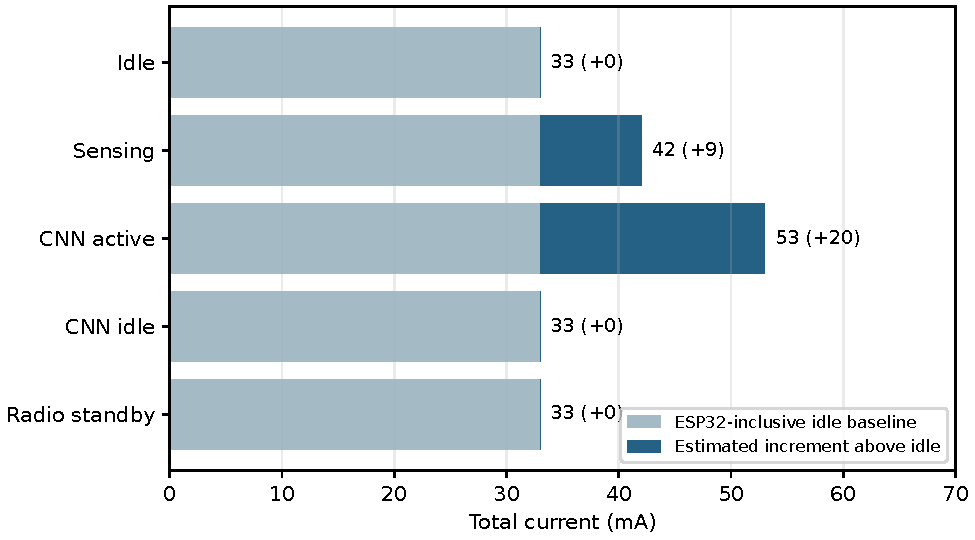
\includegraphics[width=0.9\textwidth]{figures/operating_mode_current.pdf}
\caption{\newrevision{ESP32-inclusive readings split into the 33 mA idle baseline and estimated increments. Equal indicated readings do not establish zero component consumption.}}
\label{fig:mode_current}
\end{figure}

\begin{table}[htbp]
\centering
\caption{\newrevision{LoRa transmission current at 3.3 V and calculated power and energy. Energy calculations use the full indicated current.}}
\label{tab:lora_power}
\begin{tabular}{rrrrrr}
\toprule
TX setting & Current & Power & Run energy & Packet energy & DATA energy \\
(dBm) & (mA) & (mW) & (J) & (mJ) & (mJ/byte) \\
\midrule
10 & 20 & 66 & 2.8 & 2.8 & 0.35 \\
15 & 30 & 99 & 4.2 & 4.2 & 0.52 \\
17 & 40 & 132 & 5.5 & 5.5 & 0.69 \\
19 & 60 & 198 & 8.3 & 8.3 & 1.04 \\
\bottomrule
\end{tabular}
\end{table}

\newrevision{Measurement repeatability and instrument accuracy remain unquantified. The table reports rounded energy values.}

\newrevision{Power is calculated as $P=VI$, run energy as $E=Pt$, and energy per packet as $E/N$, using a 42 s run and 1,000 transmitted packets per setting. Energy per DATA byte divides packet energy by eight, the DATA packet length in this experiment. The calculations assume the indicated current represents the run average. The measurement instrument, repetition count, radio parameters, receiver delivery count, and measurement boundary remain undocumented. The results estimate run energy and energy per transmitted packet and DATA byte.}

\begin{figure}[htbp]
\centering
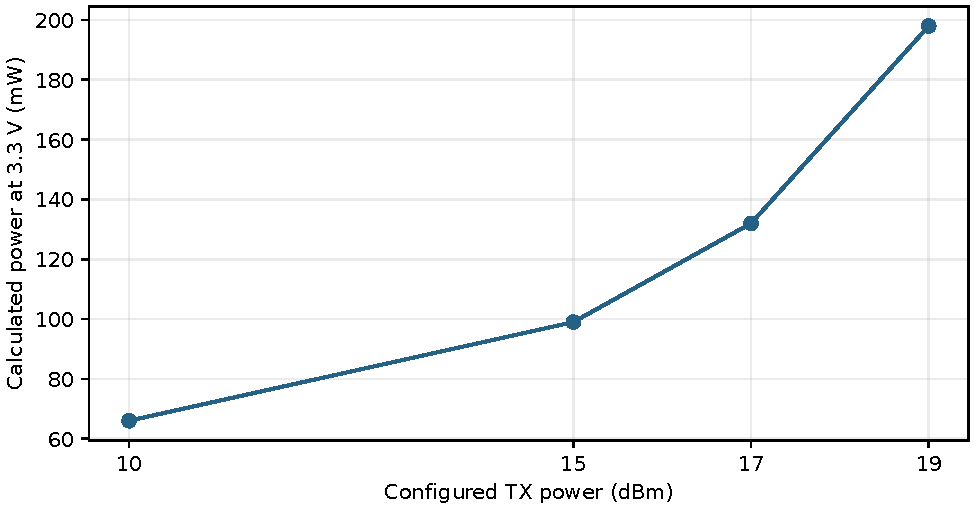
\includegraphics[width=0.9\textwidth]{figures/lora_power_sweep.pdf}
\caption{\newrevision{Calculated LoRa power at a 3.3 V supply for four transmit-power settings.}}
\label{fig:lora_power_sweep}
\end{figure}

\newrevision{Calculated power rises from 66 mW at 10 dBm to 198 mW at 19 dBm, a threefold increase. Selecting a TX setting also requires packet-delivery and range measurements under the permitted local radio settings. The 3.3 V sweep and the operating-mode measurements characterize separate test setups. Comparing their readings requires equivalent supply conditions and measurement boundaries.}
\FloatBarrier

\subsection{Communication Test Results}
\label{sec:communication_results}
\newrevision{The historical eight-byte experiment is separate from the current version-5, 34-byte result demonstration in Section~\ref{sec:communication_protocol}. The supplied \texttt{Com Logs.csv} contains 50 runs requesting 1,000 packets each. The team confirmed the test settings and packet layout in Tables~\ref{tab:communication_setup} and~\ref{tab:communication_payload}. Tests included different distances and did not have full line of sight: objects and reflective materials were present around the test area. Their individual effects were not isolated. The furthest successful communication distance reached was 350 m with the current hardware and spring antennas. This is the maximum distance reached during these tests, rather than an established maximum radio range. Individual CSV rows are not mapped to distance, and the test date remains unreported.}

\begin{table}[htbp]
\centering
\caption{\newrevision{Team-confirmed communication experiment configuration.}}
\label{tab:communication_setup}
\begin{tabular}{p{0.40\textwidth}p{0.50\textwidth}}
\toprule
Setting & Value \\
\midrule
Radio / frequency & SX1278 / 433 MHz \\
Spreading factor & SF7 \\
Bandwidth & 125 kHz \\
Coding rate & 4/5 \\
Configured TX power & 10 dBm \\
Antennas & 433 MHz spring antennas \\
Test conditions & Partial obstruction; objects and reflective materials nearby \\
\newrevision{DATA / application} & \newrevision{8 bytes / 6 bytes, synthetic records} \\
\bottomrule
\end{tabular}
\end{table}

\begin{table}[htbp]
\centering
\caption{\newrevision{Historical eight-byte DATA packet: two-byte sequence and six-byte application record.}}
\label{tab:communication_payload}
\begin{tabular}{p{0.16\textwidth}p{0.74\textwidth}}
\toprule
Byte offsets & Contents \\
\midrule
0--1 & Sequence number: unsigned 16-bit integer, little-endian \\
2 & Node ID \\
3 & Day (five bits) and battery code (three bits) \\
4--7 & Synthetic probability: \texttt{(sequence \% 101) / 100.0f}, float32, little-endian \\
\bottomrule
\end{tabular}
\end{table}

\newrevision{The probability field is generated from the sequence number; it is not a classifier prediction. These packets contain neither MFCC coefficients nor measured RPW detection results. DATA byte 3 holds day in bits 7--3 and battery in bits 2--0. The battery code is $\operatorname{round}(7\,\operatorname{clamp}(P,0,100)/100)$ for input percentage $P$; codes are 0--7. Day is 1--31. The experimental defaults (node 1, day 15, simulated battery 80\%, code 6) are not measured calendar/battery telemetry. The eight DATA bytes comprise two sequence bytes and six application bytes; PHY and control-message overhead are additional.}
\FloatBarrier

\begin{table}[htbp]
\centering
\caption{\newrevision{Summary of 50 historical eight-byte communication runs.}}
\label{tab:communication_results}
\begin{tabular}{p{0.51\textwidth}p{0.39\textwidth}}
\toprule
Measure & Result \\
\midrule
Original packets requested & 50,000 \\
Furthest distance reached (team-reported) & 350 m, current hardware and antenna \\
Initial unique packets received & 49,710 (99.42\%) \\
Initial missing packets & 290 (0.58\%) \\
Additional ARQ DATA transmissions & 290 \\
Recovered packets & 290 \\
Final unique packets received & 50,000 (100\%) \\
Final missing / reported duplicates & 0 / 0 \\
Initial loss per run & 0--2.2\% \\
Observation duration & Mean 113.147 s; range 110.483--119.138 s \\
Delivered records per second & Mean 8.869; range 8.418--9.080 \\
Logged application goodput & Mean 425.704 bit/s; range 404.040--435.853 \\
Logged DATA goodput & Mean 567.606 bit/s; range 538.721--581.137 \\
Mean send-call duration & 36.871 ms; run means 36.865--36.875 ms \\
RSSI run averages & $-103.70$ to $-52.57$ dBm \\
SNR run averages & 3.69--9.87 dB \\
\bottomrule
\end{tabular}
\end{table}

\newrevision{Automatic repeat request (ARQ) recovered all initial misses. Each run completed 1,000 original transmissions, with no locally failed/skipped records reported. Additional DATA retransmissions equal 0.58\% of original packets; this excludes control-message and acknowledgement overhead. Final delivery was 100\% in every recorded run, rather than a guarantee for other conditions.}

\begin{figure}[htbp]
\centering
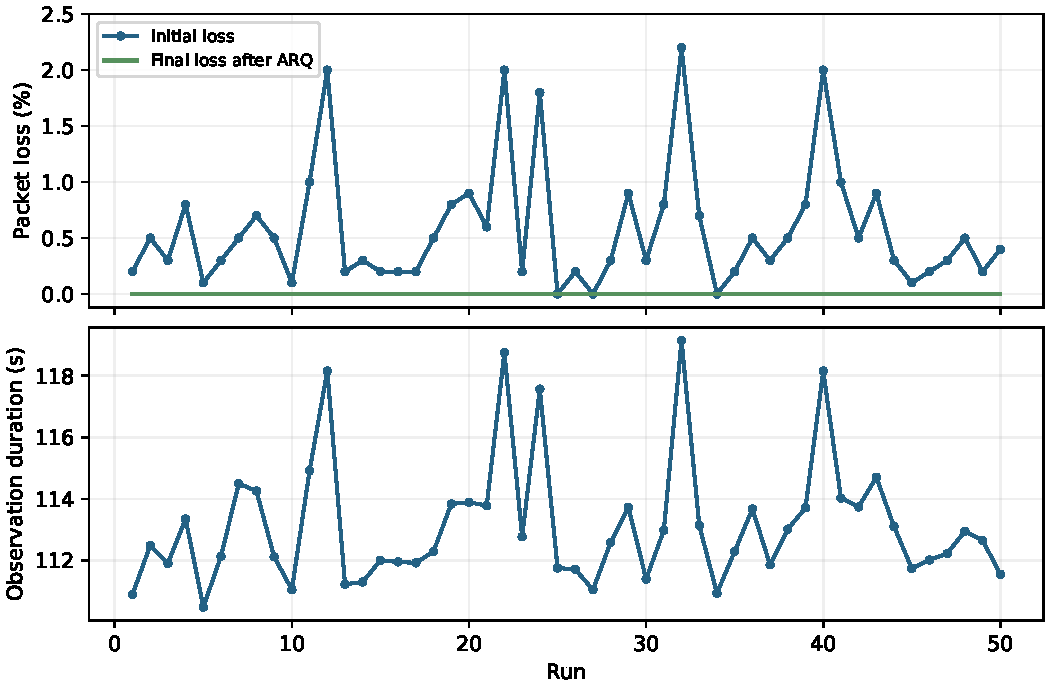
\includegraphics[width=\textwidth]{figures/communication_runs.pdf}
\caption{\newrevision{Initial/final loss and observation duration in CSV row order across tests that included different distances. Distances are not assigned to individual rows, so the horizontal axis is run number.}}
\end{figure}

\newrevision{DATA send calls total approximately 36.9--37.7 s per run, while receiver observation averages approximately 113 s. Send-call duration is not end-to-end latency. The historical Control-Fix scheduler reserves 125 eight-record windows of 872 ms (109 s) plus a fixed 10 s retry allowance, giving a 119 s single-session assignment. The reported timing is consistent with that configuration; the 50-run binary/build provenance still needs confirmation. This is unrelated to the current 1,099 ms per-node slot. Overrun compares actual sender slot elapsed with the fixed assignment on the sender clock, excluding START setup and final END reporting. Receiver START-to-first-END observation has different boundaries: a 119.138 s observation does not establish overrun when the corresponding sender schedule is about 118.8 s. Runs continue after the assignment for measurement and must report the sender overrun flag.}

\newrevision{Logger definitions are available from the experimental source. For $U$ final unique valid records and actual sender slot elapsed $T$ seconds, delivered records/s is $U/T$, application goodput is $48U/T$ bit/s and DATA goodput is $64U/T$ bit/s. Retries and control delays contribute to $T$ but their bytes are not additional useful delivery. The 48:64 ratio agrees with the six- versus eight-byte definitions. These are neither 34-byte-demo nor compressed-MFCC throughput measurements. Means are arithmetic run averages across the combined tests; RSSI/SNR ranges describe run averages, not instantaneous extremes. Without a run-to-distance mapping, these aggregate delivery and throughput values cannot be assigned specifically to 350 m or used to plot performance versus distance. These logs demonstrate packet reception and recovery but do not establish Wi-Fi/cloud forwarding or classifier and codec correctness. The power experiment also used eight-byte packets. Its 42 s run duration differs from the communication-log observation durations, so combining the energy and delivery results still requires matched timing and measurement boundaries. Per-run distances, radio airtime, and end-to-end latency remain pending.}
\FloatBarrier

\subsection{\newrevision{Offline MFCC Compression-Size Results}}
\label{sec:codec_results}
\begingroup
\color{green!45!black}
The team-supplied \texttt{compression.md} summarizes \nolinkurl{recording_size_comparison.csv}: 58,797 recordings, with six size observations per recording. The handoff reports no missing size values or duplicate source/path keys. The underlying CSV and optimization artifacts were not supplied with this report update, so these statistics are reproduced from the handoff rather than independently recomputed.

\begin{table}[htbp]
\centering
\color{green!45!black}
\small
\caption{\newrevision{Offline recording counts and supplied split labels.}}
\label{tab:codec_counts}
\begin{tabular}{lrrrrr}
\toprule
Source & Train & Validation & Test & Total & Int8 values \\
\midrule
Lab & 32,729 & 10,957 & 10,957 & 54,643 & 10,655,385 \\
Field & 1,434 & 427 & 2,293 & 4,154 & 810,030 \\
Total & 34,163 & 11,384 & 13,250 & 58,797 & 11,465,415 \\
\bottomrule
\end{tabular}
\end{table}

The distributions pool training, validation, and test recordings. They describe full-dataset sizes, not held-out generalization: the bank-construction process and group separation are not established by the handoff. Values exclude eight metadata bytes under the offline experiment's convention. They are not verified on-air payload lengths, and adding the current six-byte header to them would require matching the original codec and packing rules.

\begin{table}[htbp]
\centering
\color{green!45!black}
\small
\caption{\newrevision{Lab compression sizes in bytes, excluding eight metadata bytes (54,643 recordings).}}
\label{tab:codec_lab}
\begin{tabular}{lrrrrrr}
\toprule
Bank & Mean & Median & P90 & P95 & P99 & Max \\
\midrule
Balanced 2 & 46.27 & 46 & 48.0 & 49 & 51 & 68 \\
Field-only 1 & 49.19 & 49 & 51.0 & 52 & 53 & 68 \\
Field-only 2 & 47.01 & 47 & 49.0 & 50 & 51 & 69 \\
Field-only 4 & 46.40 & 46 & 49.0 & 49 & 51 & 68 \\
Field-only 8 & 46.51 & 46 & 49.0 & 49 & 51 & 68 \\
Field-only 16 & 46.64 & 47 & 49.0 & 49 & 51 & 68 \\
\bottomrule
\end{tabular}
\end{table}

\begin{table}[htbp]
\centering
\color{green!45!black}
\small
\caption{\newrevision{Field compression sizes in bytes, excluding eight metadata bytes (4,154 recordings).}}
\label{tab:codec_field}
\begin{tabular}{lrrrrrr}
\toprule
Bank & Mean & Median & P90 & P95 & P99 & Max \\
\midrule
Balanced 2 & 65.81 & 64 & 81.7 & 87 & 102 & 140 \\
Field-only 1 & 66.90 & 63 & 84.0 & 91 & 109 & 151 \\
Field-only 2 & 65.66 & 64 & 81.0 & 87 & 101 & 140 \\
Field-only 4 & 65.30 & 64 & 80.0 & 85 & 96 & 128 \\
Field-only 8 & 65.20 & 63 & 80.0 & 85 & 94 & 117 \\
Field-only 16 & 65.20 & 63 & 80.0 & 85 & 94 & 119 \\
\bottomrule
\end{tabular}
\end{table}
\FloatBarrier

\begin{figure}[htbp]
\centering
\color{green!45!black}
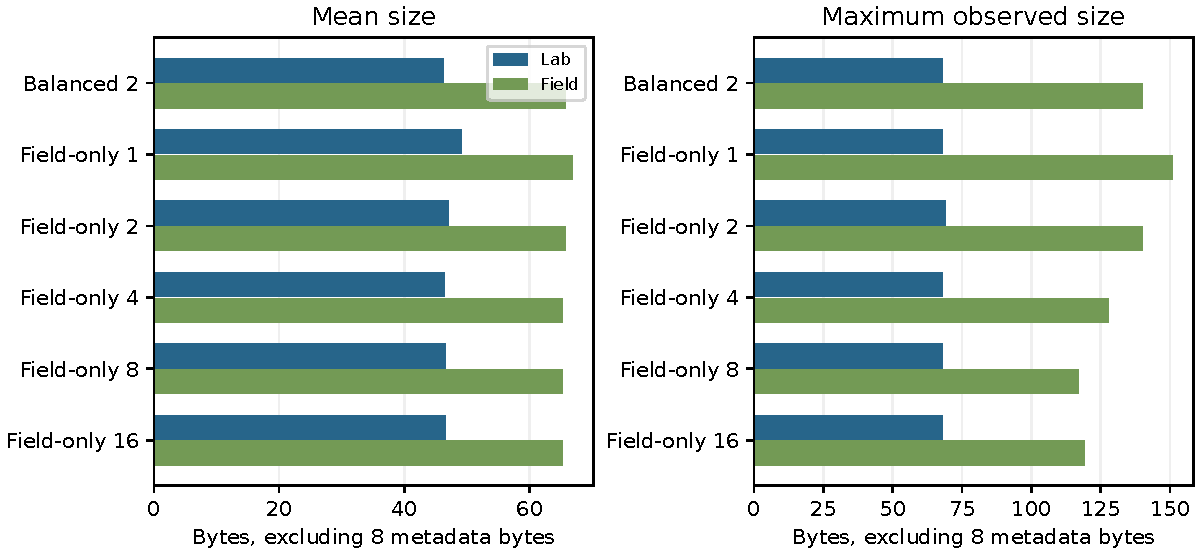
\includegraphics[width=\linewidth]{figures/compression_bank_summary.pdf}
\caption{\newrevision{Offline bank comparison reproduced from the supplied summary. Left: mean size; right: maximum observed size. Both exclude eight metadata bytes and pool all dataset splits.}}
\label{fig:codec_bank_summary}
\end{figure}
\FloatBarrier

Balanced 2 has the lowest lab mean (46.27 B); Field-only 8 averages 46.51 B. On field recordings, Field-only 8 averages 65.20 B and has a maximum of 117 B, compared with 65.81 B and 140 B for Balanced 2. Field-only 16 has the same rounded field mean but a maximum of 119 B. Field sizes are higher and more dispersed; these distributions alone do not identify a causal noise mechanism.

\begin{table}[htbp]
\centering
\color{green!45!black}
\small
\caption{\newrevision{Paired size comparison on the same recordings. Negative mean difference favors Field-only 8.}}
\label{tab:codec_paired}
\begin{tabular}{lrrrr}
\toprule
Source & Field-only 8 smaller & Equal & Balanced 2 smaller & Mean difference (B) \\
\midrule
Lab & 320 & 40,951 & 13,372 & $+0.238$ \\
Field & 1,522 & 2,082 & 550 & $-0.618$ \\
\bottomrule
\end{tabular}
\end{table}

For accounting only, an uncompressed $15\times13$ float32 matrix occupies 780 B; int8 coefficients occupy 195 B, or 199 B with a float32 scale. A hypothetical raw-int8 packet with the six-byte application header would occupy 201 B, since that header already includes the scale. These are arithmetic baselines, not additional measured CSV variants. The supplied comparison does not establish raw/int4/fixed-$k$/Huffman benchmark results, classifier accuracy, quantization error, ESP32 runtime or memory use, airtime, RF delivery, or battery savings.
\endgroup
\FloatBarrier


\section{Performance Analysis Plan}
\label{sec:PerformanceAnalysisPlan}

\newrevision{Results will be compared across the distance, amplitude, and noise conditions in Section~\ref{sec:Testing}, using the metrics in Section~\ref{sec:PerformanceMetrics}.}

\newrevision{The communication analysis will compare baseline features, compact features, and classification-result packets. It will report payload bytes, airtime, packet loss, and energy, together with ESP32 memory and runtime for the corresponding processing path. A smaller packet is useful only when it preserves the required detection performance.}

\chapter{Project Management}
\label{ch:ProjectManagement}

% ===============================
% CHAPTER 7: PROJECT MANAGEMENT
% ===============================

\section{Life Cycle Model}
\label{sec:SWLifecycle}

\subsection{Overview and Rationale}

\earlierrevision{The project combines hardware, embedded firmware, wireless networking, cloud software, and machine learning. Each subsystem depends on experimental results, especially sensor coupling, outdoor noise, communication reliability, and model performance. The team therefore uses an Agile-Spiral hybrid: each spiral addresses a major technical risk, while short iterations produce and test a working increment.}

\subsection{Model Structure and Phases}

The Agile-Spiral life cycle adopted for this project consists of five major spiral iterations, each structured around four quadrants consistent with Boehm's original Spiral Model formulation: (1) Determine objectives, (2) Identify and resolve risks, (3) Develop and test, and (4) Plan the next iteration. Within the development and test quadrant of each spiral, Agile sprint cycles of two to three weeks are conducted to produce testable increments of the system.

\earlierrevision{The five spiral iterations cover the six design objectives in Section 1.4. Objectives 4 and 5 are combined in the integration and field-validation spiral, while Objective 6 is delivered through the deployment guides and calibration procedures produced at the end of that spiral.}

\begin{table}[h!]
\centering
\caption{Agile-Spiral Iteration Plan}
\label{tab:spiral_plan}
\renewcommand{\arraystretch}{1.3}
\begin{tabular}{>{\raggedright\arraybackslash}p{2.2cm} >{\raggedright\arraybackslash}p{3.8cm} >{\raggedright\arraybackslash}p{3.8cm} >{\raggedright\arraybackslash}p{1.8cm}}
\toprule
\textbf{Spiral / Phase} & \textbf{Primary Objectives} & \textbf{Key Deliverables} & \textbf{Duration} \\
\midrule
Spiral 1: Requirements \& Architecture &
Finalize system architecture; define sensor node hardware specifications; establish dataset and labeling strategy &
System architecture diagram; hardware BoM; dataset acquisition plan &
3 weeks \\
Spiral 2: Acoustic Sensing Unit &
Prototype piezoelectric sensing node; calibrate the mechanical exciter and reference sensor; run controlled wood-plank trials; implement bandpass filtering pipeline &
\newrevision{Functional sensor node prototype; calibrated bench apparatus; controlled wood-plank test report} &
4 weeks \\
Spiral 3: Wireless Sensor Network &
Implement WSN architecture; compare baseline and compact LoRa packets; optimize power management; environmental enclosure &
\newrevision{Communication reliability report; packet-compaction comparison; power consumption analysis} &
4 weeks \\
Spiral 4: Deep Learning Classifier &
Train and validate CNN/BiLSTM/hybrid classifiers on TreeVibes dataset; optimize hyperparameters; 10-fold cross-validation &
\newrevision{Selected classification model; confusion matrix; recall, false-negative rate, F1 score, and cross-validation variance report} &
5 weeks \\
Spiral 5: Integration \& Field Validation &
Cloud platform integration; dashboard development; end-to-end testing; live-palm validation only where naturally infested palms are available &
\newrevision{Monitoring dashboard; bench-validation report; live-palm validation report only if available; final performance metrics} &
4 weeks \\
\bottomrule
\end{tabular}
\end{table}

\newrevision{The phase gate after the wood-plank campaign requires the team to review playback fidelity, SNR versus distance, and recall versus distance/noise before making a live-palm claim. If naturally infested palms are unavailable, the team will complete the emulation study and report it as controlled bench validation rather than as proof of real RPW detection.}

\FloatBarrier

\subsection{Agile Practices Within Each Spiral Iteration}

Within each spiral iteration, the development team applies core Agile engineering practices to manage task decomposition, progress tracking, and quality assurance. These include:

\begin{itemize}
    \item \textbf{Sprint Planning:} At the start of each two-to-three-week sprint, team members
    identify and assign user stories and engineering tasks relevant to the active spiral
    objective. Tasks are drawn from a maintained product backlog and prioritized based on
    risk criticality and functional dependencies.

    \item \textbf{Iterative Prototyping and Testing:} Hardware and software components are built in
    small, testable increments. Each sprint concludes with a working prototype or testable
    software module. This enables rapid detection of integration failures. For instance,
    incompatibility between the microcontroller sampling rate and the cloud preprocessing
    pipeline before they propagate to later development stages.

    \item \earlierrevision{\textbf{Continuous Integration and Validation:} Automated training and evaluation scripts
    are run after changes to the model or data pipeline. Recall is the primary selection metric,
    with false-negative rate, precision, F1 score, and data-split variance reported alongside it.}

    \item \textbf{Sprint Review and Retrospective:} Each sprint concludes with a structured review in
    which completed increments are demonstrated to advisors (Dr. Mohamed Alhajri and Dr.
    Taha Landolsi) for validation against the project objectives. A retrospective session
    identifies process impediments and adjusts task allocation for the subsequent sprint.

    \item \textbf{Risk Register Maintenance:} Consistent with the Spiral Model's risk-driven
    approach, a living risk register is maintained throughout the project. Risks identified
    during each spiral, including environmental noise interference, sensor calibration drift,
    and wireless packet loss under field conditions are formally assessed, prioritized, and
    mitigated before progressing to the next iteration.
\end{itemize}

\newrevision{The iteration plan maps sensing, networking, classification, integration, and deployment work to the design objectives in Section 1.4.}

\section{Work Breakdown Structure}
\label{sec:WBS}

\subsection{Top Level Work}

\earlierrevision{The Work Breakdown Structure (WBS) divides the project into five packages: (1) Requirements \& Architecture, (2) Acoustic Sensing Unit, (3) Wireless Sensor Network, (4) Deep Learning Classifier, and (5) Integration \& Field Validation. Together, these packages cover the design, implementation, and validation of the complete prototype. The following subsections summarize the purpose and outputs of each package.}

\begin{figure}[H]
\centering
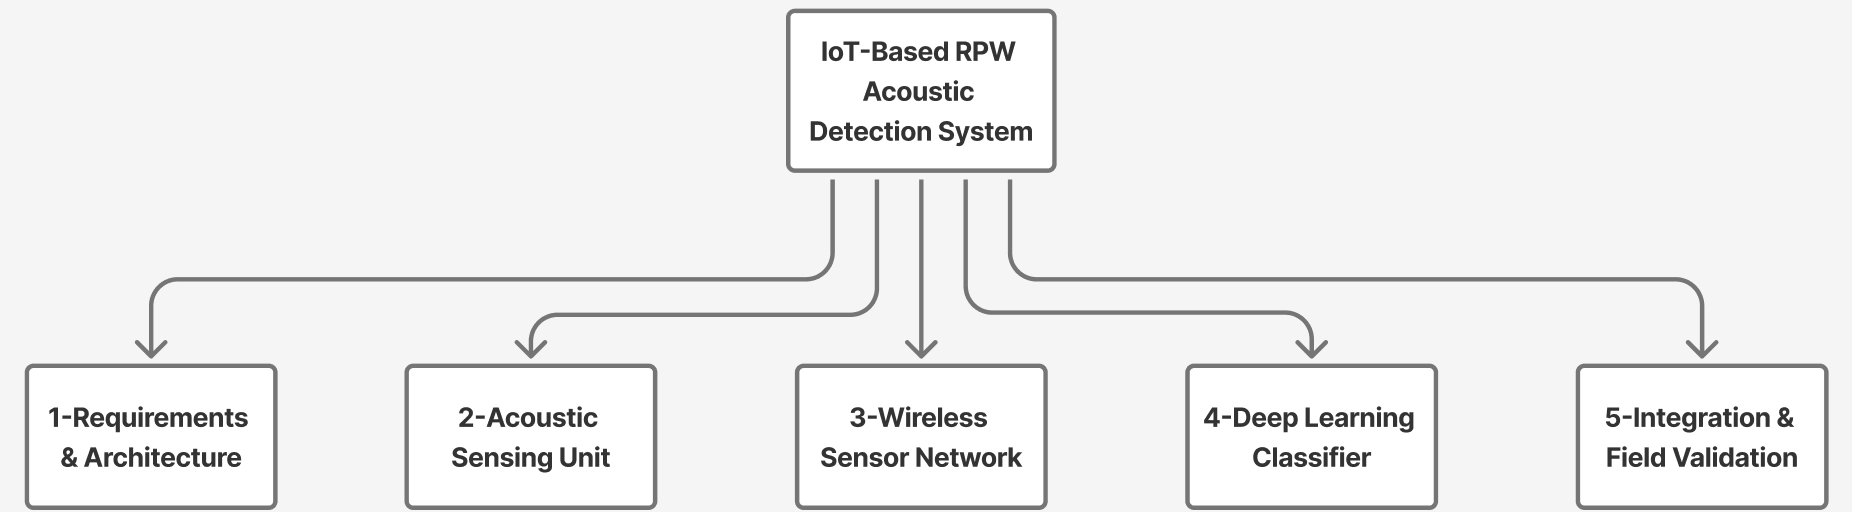
\includegraphics[width=0.85\textwidth]{figures/TLP.png}
\caption{Top Level Breakdown}
\label{fig:wbs_toplevel}
\end{figure}

\subsection{WP1 --- Requirements \& Architecture}

This work package establishes the technical and operational foundation for the entire system. It encompasses four tasks: defining the overall system architecture and interface specifications; preparing the hardware bill of materials; planning the acoustic dataset acquisition process; and designing the labeling strategy that will guide supervised model training. Outputs from this package directly inform all subsequent work packages.

\begin{figure}[H]
\centering
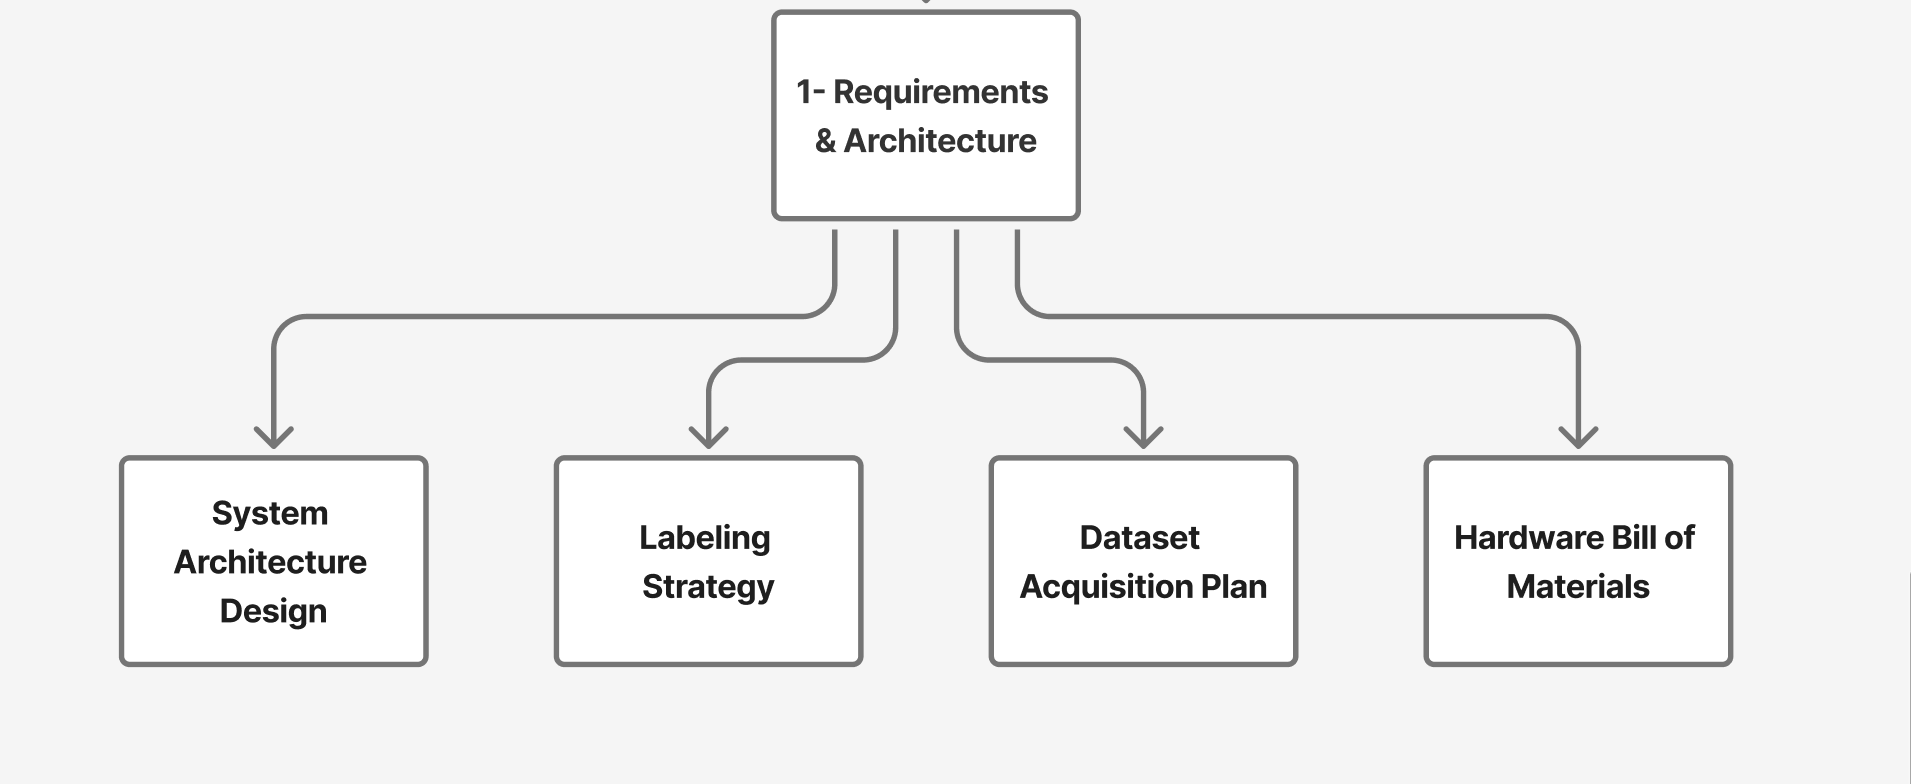
\includegraphics[width=0.85\textwidth]{figures/WP1.png}
\caption{WP1 --- Requirements \& Architecture}
\label{fig:wbs_wp1}
\end{figure}

\subsection{WP2 --- Acoustic Sensing Unit}

The Acoustic Sensing Unit translates RPW mechanical vibrations inside palm tree trunks into clean electrical signals ready for wireless transmission. The five tasks span hardware prototyping of piezoelectric sensors, plate-assisted surface coupling, construction of the signal acquisition pipeline, implementation of bandpass filters to isolate the RPW frequency band, and a controlled lab validation campaign to confirm performance before field deployment.

\begin{figure}[H]
\centering
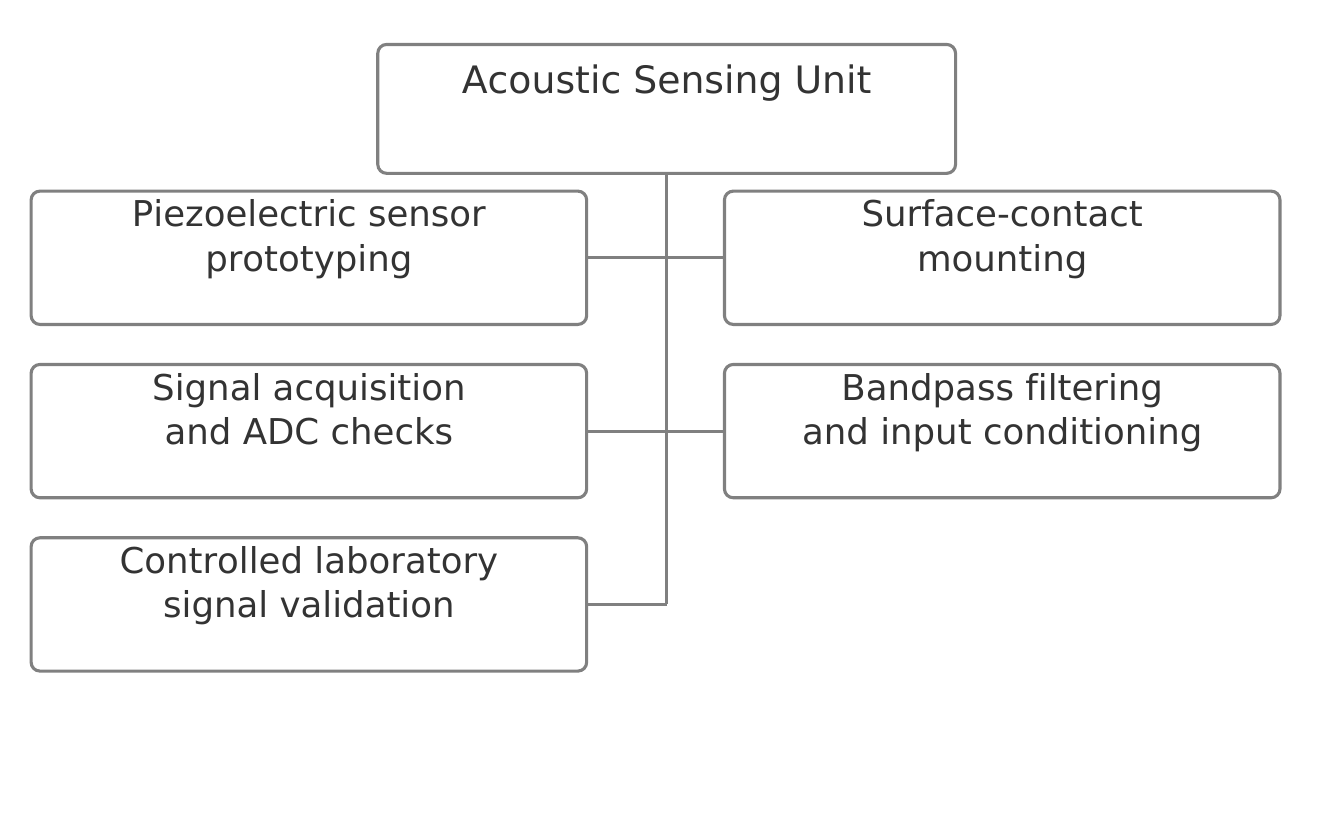
\includegraphics[width=0.85\textwidth]{figures/WP2.png}
\caption{WP2 --- Acoustic Sensing Unit}
\label{fig:wbs_wp2}
\end{figure}

\subsection{WP3 --- Wireless Sensor Network}

The Wireless Sensor Network (WSN) package ensures that acoustic data collected by individual sensing nodes is reliably transmitted to the cloud processing backend. Tasks address WSN topology design, selection and configuration of LoRa communication modules, power management strategies for extended battery life in remote plantations, weatherproof enclosure design, and the multi-node deployment and integration tests that confirm network-wide reliability.

\begin{figure}[H]
\centering
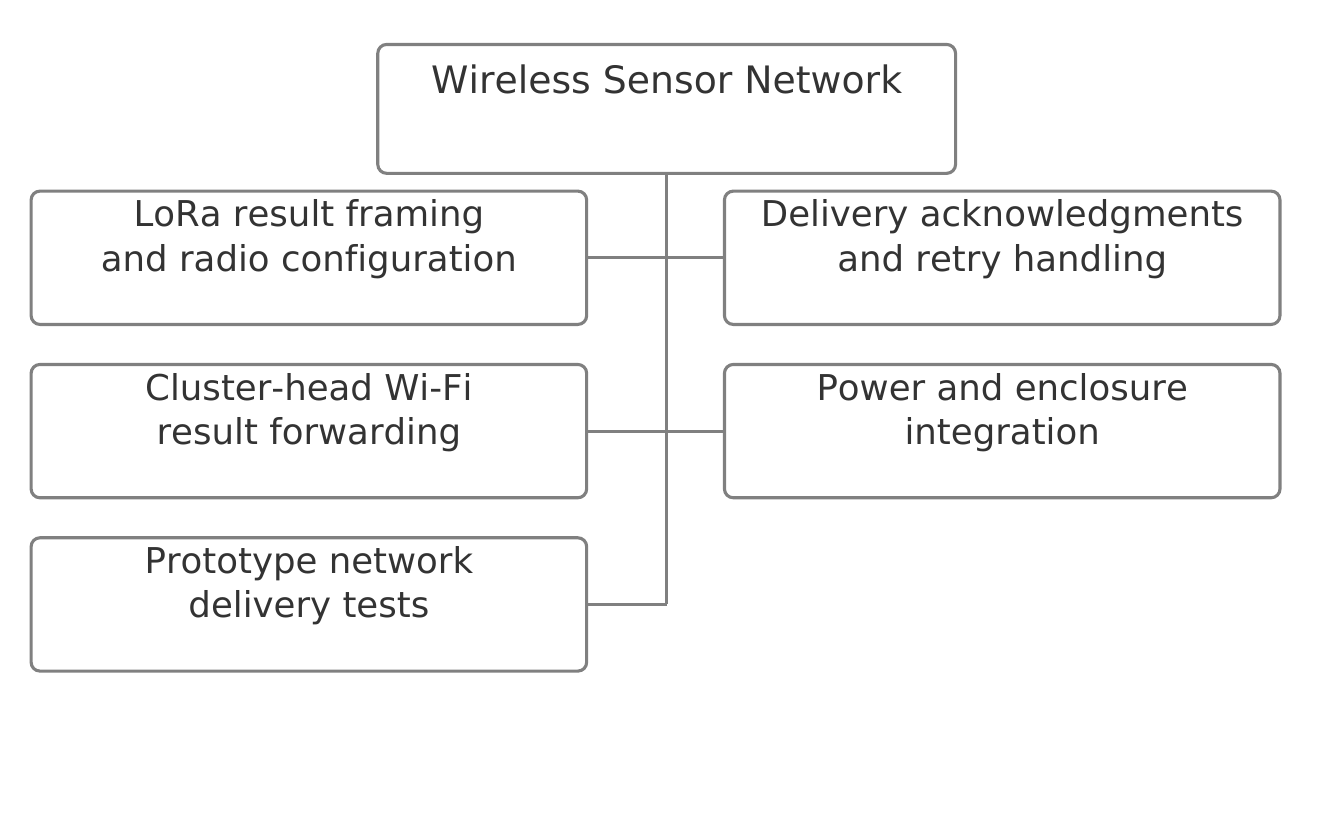
\includegraphics[width=0.85\textwidth]{figures/WP3.png}
\caption{WP3 --- Wireless Sensor Network}
\label{fig:wbs_wp3}
\end{figure}

\subsection{WP4 --- Deep Learning Classifier}

The Deep Learning Classifier is the intelligence core of the system. It processes raw acoustic data through a multi-stage pipeline: data preprocessing and augmentation to improve model generalization; feature extraction using four complementary spectral representations; and training of three candidate model architectures --- CNN Transfer Learning, BiLSTM, and a CNN-LSTM Hybrid. Hyperparameter tuning and 10-fold cross-validation ensure rigorous, reproducible performance estimation. Task 4.2 (Feature Extraction) is further broken down into four sub-tasks covering MFCC, BFCC, CQCC, and STFT Spectrogram methods.

\begin{figure}[H]
\centering
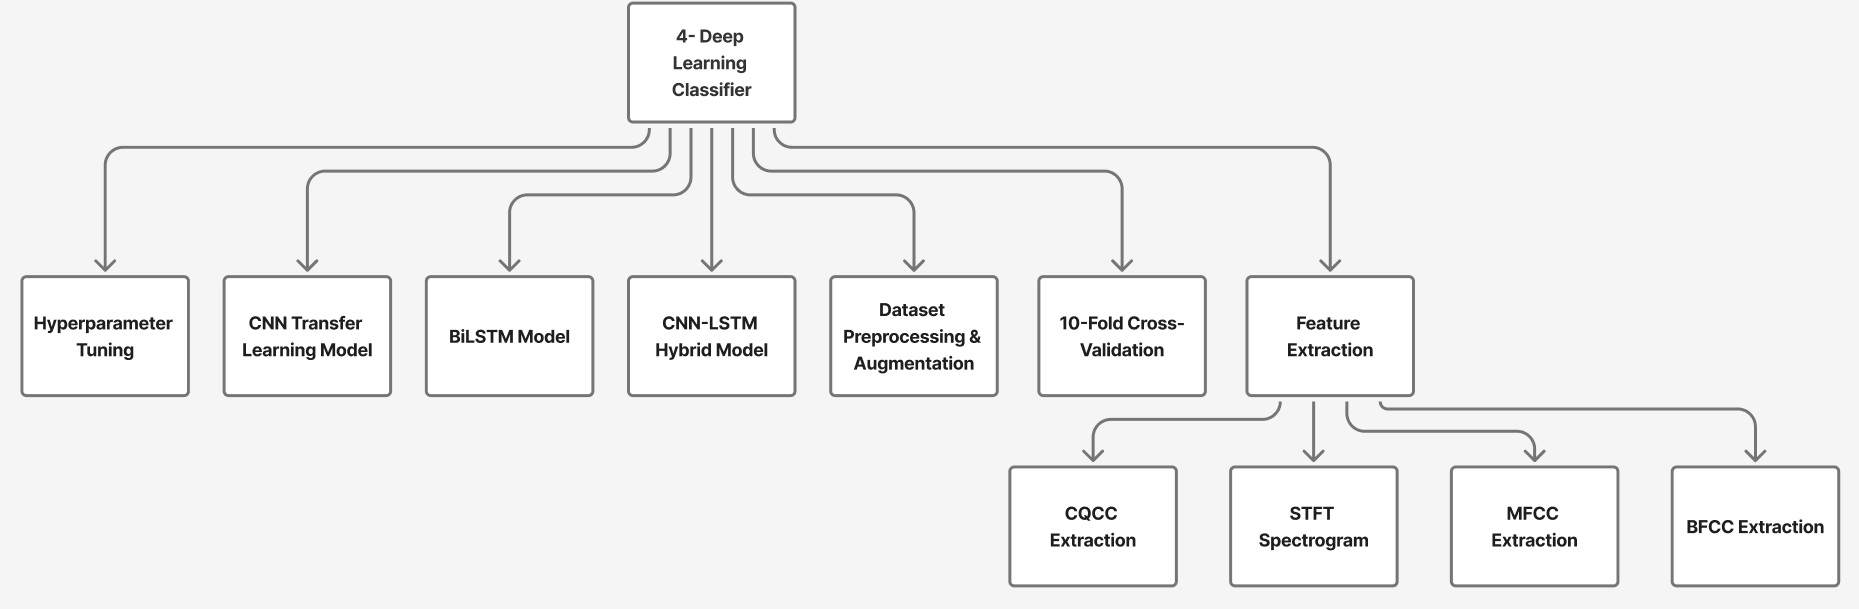
\includegraphics[width=0.85\textwidth]{figures/WP4.png}
\caption{WP4 --- Deep Learning Classifier}
\label{fig:wbs_wp4}
\end{figure}

\subsection{WP5 --- Integration \& Field Validation}

The final work package closes the loop by deploying the full system end-to-end in real agricultural environments. Seven tasks cover cloud infrastructure provisioning, automated preprocessing pipelines, the model inference and alert engine, a real-time monitoring dashboard for farm operators, field deployment and sensor calibration at palm plantation sites, holistic end-to-end system validation, and a head-to-head comparative analysis against conventional manual inspection methods to quantify the detection advantages offered by the IoT solution.

\begin{figure}[H]
\centering
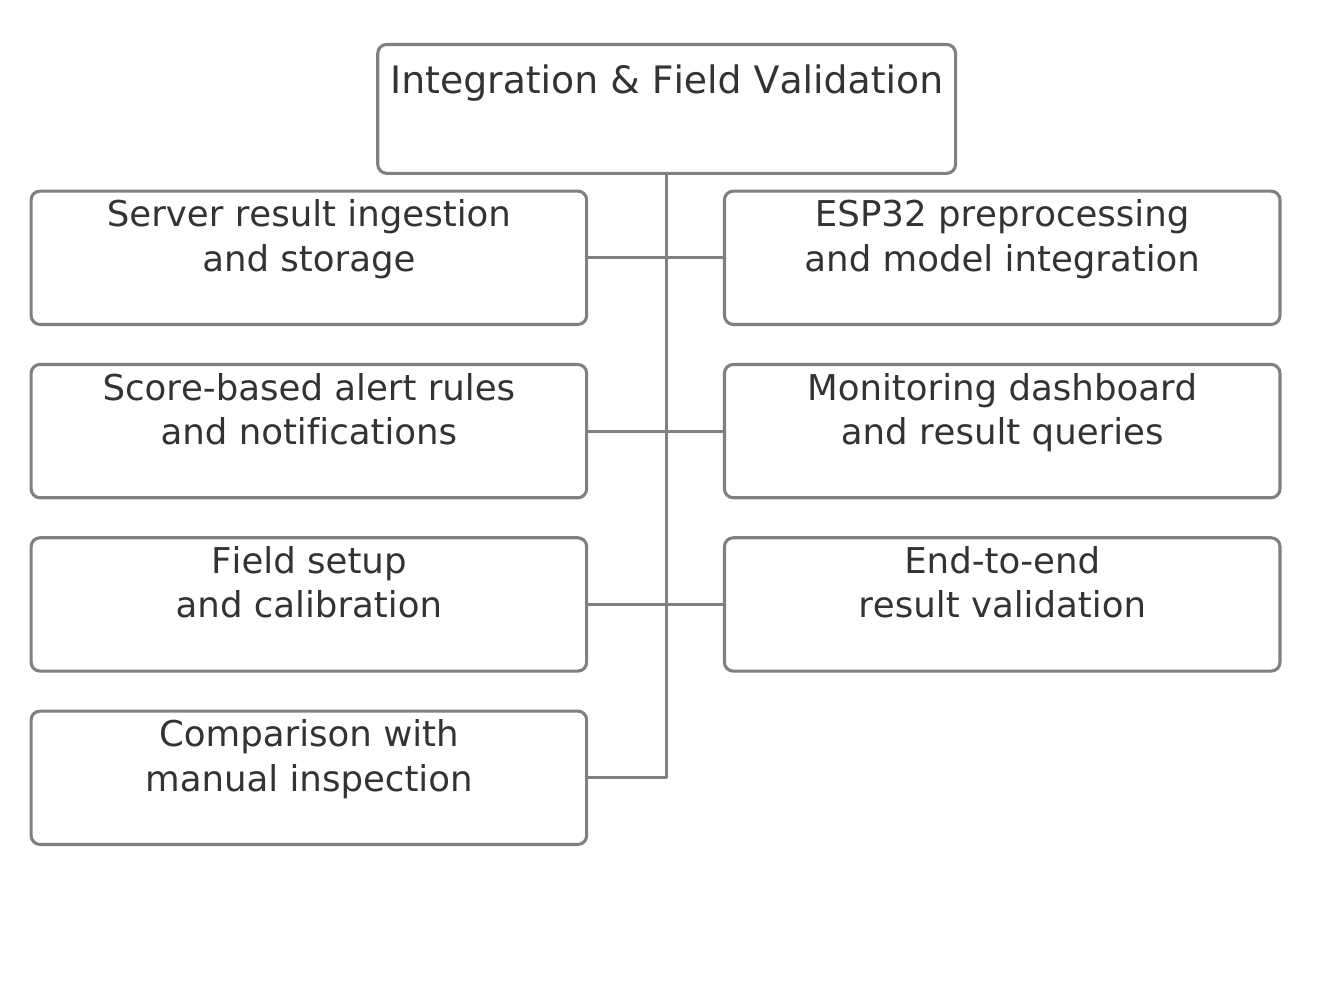
\includegraphics[width=0.85\textwidth]{figures/WP5.png}
\caption{WP5 --- Integration \& Field Validation}
\label{fig:wbs_wp5}
\end{figure}

\section{Project Schedule and Resource Assignments (Gantt Chart)}
\label{sec:Schedule}

\earlierrevision{The original planning schedule covers six objectives from January to June 2026. Senior Design II implementation is now in progress; this historical plan does not indicate current completion dates. Revised dates and completion status remain to be supplied. Some tasks overlap so that hardware, networking, and machine-learning work can progress in parallel, while integration tasks depend on earlier prototype outputs. Table~\ref{tab:gantt} assigns a lead, support member where needed, and a delivery window to each task. Progress is reviewed weekly, and delays that affect integration are recorded in the risk register and reflected in the next iteration plan.}

\renewcommand{\arraystretch}{1.3}
\begin{longtable}{>{\raggedright\arraybackslash}p{6.5cm} >{\raggedright\arraybackslash}p{2.8cm} >{\raggedright\arraybackslash}p{1.8cm} >{\raggedleft\arraybackslash}p{1.8cm}}
\caption{RPW Detection System --- Original Project Schedule with Resource Assignments (January -- June 2026)}\label{tab:gantt}\\
\toprule
\textbf{Task / Deliverable} & \textbf{Schedule} & \textbf{Lead} & \textbf{Support} \\
\midrule
\multicolumn{4}{l}{\textbf{O1 $\cdot$ Acoustic Sensing Unit (Spiral 1--2)}} \\
Physical Sensor Assembly \& Surface Mounting & Jan 19 -- Feb 2 & Abdurrahman & --- \\
MCU Programming \& ADC Sampling & Jan 19 -- Feb 2 & Khalid & --- \\
Analog Signal Conditioning \& Pre-filtering & Jan 26 -- Feb 5 & Khalid & --- \\
Bandpass Filter Pipeline 100--2500 Hz & Feb 2 -- Feb 9 & Khalid & --- \\
Outdoor Enclosure \& Rugged Casing & Feb 2 -- Feb 9 & Abdurrahman & --- \\
Lab Signal Validation & Feb 9 -- Feb 16 & Abdurrahman & Khalid \\
\midrule
\multicolumn{4}{l}{\textbf{O2 $\cdot$ Wireless Sensor Network (Spiral 3)}} \\
WSN Topology \& Protocol Design & Feb 16 -- Feb 23 & Kareem & --- \\
LoRa Module Config \& Packet Formatting & Feb 23 -- Mar 5 & Kareem & --- \\
MCU $\leftrightarrow$ Wireless Firmware \& Scheduling & Feb 23 -- Mar 5 & Khalid & Kareem \\
Battery \& Power Regulation Circuit & Feb 23 -- Mar 2 & Abdurrahman & --- \\
Network Reliability \& Sync Testing & Mar 9 -- Mar 16 & Kareem & Abdurrahman, Khalid \\
\midrule
\multicolumn{4}{l}{\textbf{O3 $\cdot$ Deep Learning Classifier (Spiral 4)}} \\
Dataset Preprocessing \& Augmentation & Mar 16 -- Mar 23 & Khalid & --- \\
Feature Extraction --- MFCC / BFCC / CQCC / STFT & Mar 16 -- Mar 26 & Khalid & --- \\
CNN Transfer Learning Model & Mar 23 -- Apr 2 & Haitham & --- \\
BiLSTM Model Architecture & Mar 23 -- Apr 2 & Haitham & --- \\
CNN-LSTM Hybrid Model & Apr 6 -- Apr 13 & Haitham & Khalid \\
Hyperparameter Tuning & Apr 13 -- Apr 20 & Haitham & Khalid \\
10-Fold Cross-Validation (variance $<$ 3\%) & Apr 13 -- Apr 20 & Haitham & Khalid \\
\midrule
\multicolumn{4}{l}{\textbf{O4 $\cdot$ Cloud Platform \& Dashboard (Spiral 5)}} \\
Cloud Server Setup \& Data Ingestion API & Apr 20 -- Apr 27 & Kareem & --- \\
Database Schema \& Security Setup & Apr 20 -- Apr 25 & Kareem & --- \\
Model Inference Service Deployment & Apr 27 -- May 4 & Haitham & --- \\
Automated Preprocessing on Server & Apr 27 -- May 4 & Haitham & --- \\
Alert Threshold Logic \& Delivery & May 4 -- May 9 & Kareem & Haitham \\
Monitoring Dashboard UI & May 4 -- May 11 & Kareem & --- \\
\midrule
\multicolumn{4}{l}{\textbf{O5 $\cdot$ Field Testing \& Validation}} \\
Hardware Durability \& Weatherproofing Checks & May 11 -- May 18 & Abdurrahman & --- \\
Network Stability \& Latency Logging & May 11 -- May 18 & Kareem & --- \\
Signal Quality \& Noise Benchmarking & May 11 -- May 18 & Khalid & --- \\
Model Accuracy vs Manual Inspection & May 11 -- May 18 & Haitham & --- \\
End-to-End System Validation & May 18 -- May 25 & All & --- \\
\midrule
\multicolumn{4}{l}{\textbf{O6 $\cdot$ Field Deployment \& Calibration}} \\
Physical Installation \& Mounting Guide & May 25 -- May 30 & Abdurrahman & --- \\
Network Configuration \& Expansion Guide & May 25 -- May 30 & Kareem & --- \\
Sensor Calibration \& Signal Verification Procedure & May 25 -- May 30 & Khalid & --- \\
Model Retraining \& Update Procedure & May 25 -- May 30 & Haitham & --- \\
End-to-End Integration Guide & May 28 -- Jun 2 & Khalid & Kareem \\
\bottomrule
\multicolumn{4}{l}{\footnotesize Note: ``Lead'' denotes the primary responsible team member; ``Support'' indicates a secondary} \\
\multicolumn{4}{l}{\footnotesize contributor. A dash (---) indicates no supporting member was assigned for that task.} \\
\end{longtable}

\clearpage
\begin{landscape}
\thispagestyle{plain}
\begin{figure}[p]
\centering
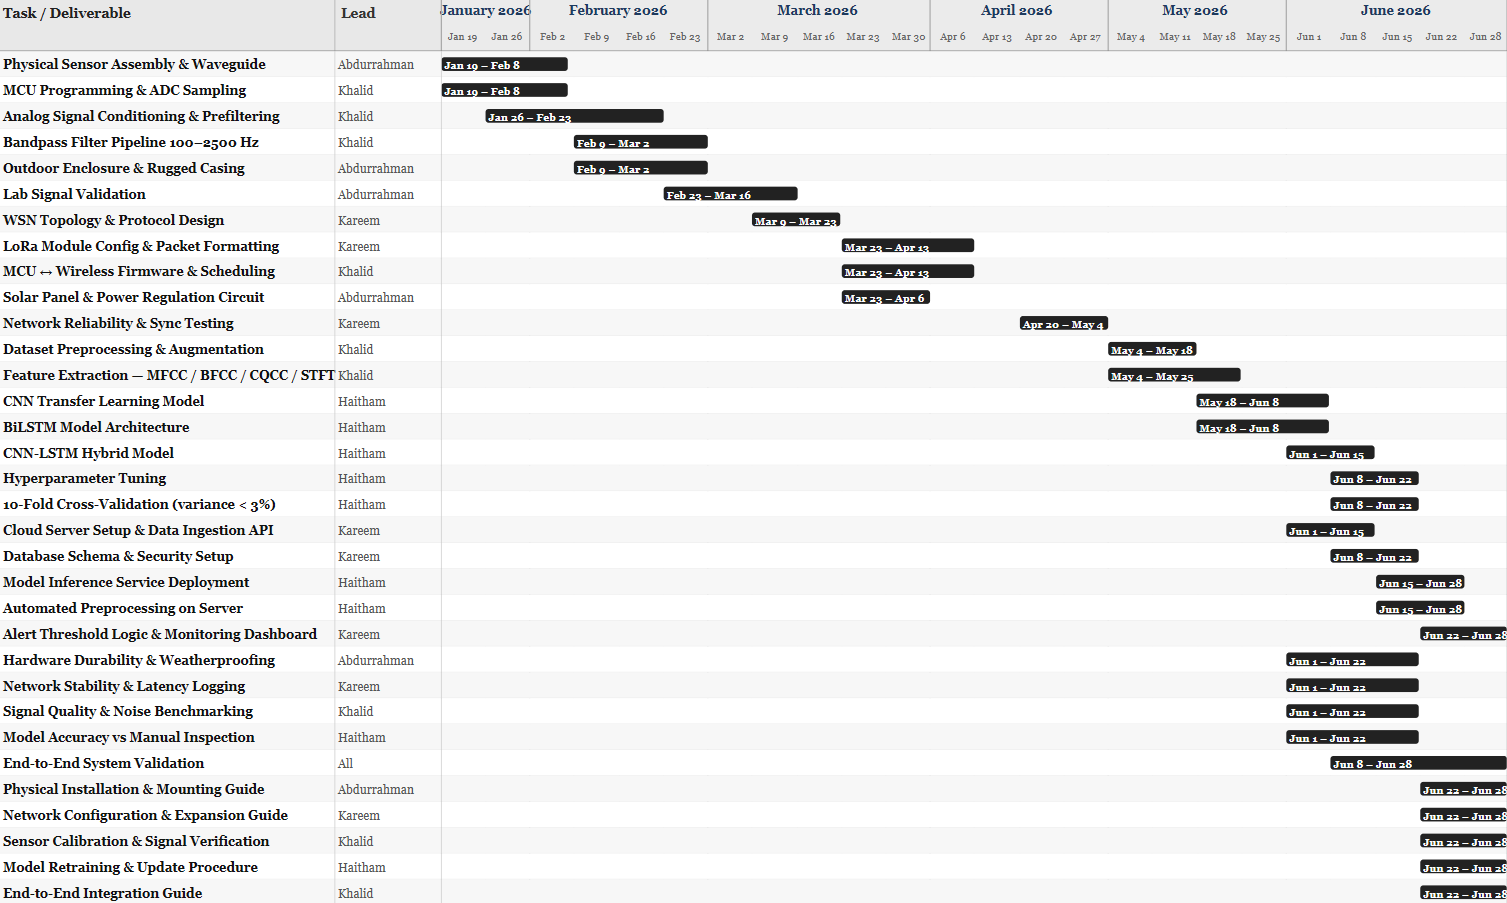
\includegraphics[width=\linewidth,height=1.12\textheight,keepaspectratio]{figures/The Gantt Chart.png}
\caption{Project Gantt Chart}
\label{fig:gantt_chart}
\end{figure}
\end{landscape}
\clearpage
\section{Team Organization}
\label{sec:TeamOrg}

\earlierrevision{The team includes three Computer Engineering students---Khalid Hamdan, Kareem Mahmoud, and Abdurrahman Maricar---and one Computer Science student, Haitham Ayyash. Their combined experience covers embedded systems, wireless networking, cloud software, and deep learning.}

\earlierrevision{The team uses a flat decision-making structure. Each member leads assigned technical work and presents progress, evidence, and blockers at the weekly meeting. Decisions are made by team consensus and reviewed with the project advisors, Dr. Mohamed Alhajri and Dr. Taha Landolsi, when they affect scope, safety, or major design choices.}

\earlierrevision{The role tables use three labels. A \emph{Lead} coordinates an objective and is accountable for its acceptance criteria. \emph{Support} contributes to work led by another member. An \emph{Owner} is accountable for a clearly bounded task within a shared objective. During field testing and deployment, all members are owners of different tasks in their own areas; this does not mean that every member owns the entire objective.}

\begin{table}[H]
\centering
\caption{Khalid Hamdan --- Roles and Responsibilities}
\label{tab:roles_khalid}
\renewcommand{\arraystretch}{1.3}
\begin{tabular}{>{\raggedright\arraybackslash}p{3.5cm} p{1.8cm} p{8.0cm}}
\toprule
\textbf{Objective} & \textbf{Role} & \textbf{Tasks} \\
\midrule
Acoustic Sensing Unit & Support & Microcontroller programming; ADC sampling rate
configuration; analog signal conditioning circuitry; on-device
pre-filtering pipeline \\
Wireless Sensor Network & Support & MCU wireless module firmware; buffering and transmission
scheduling logic \\
Deep Learning Classifier & Lead & Signal preprocessing pipeline; feature extraction (MFCC,
BFCC, CQCC, STFT spectrograms); dataset preparation and
augmentation; TinyML edge inference feasibility study \\
Field Testing \& Validation & Owner & Signal quality validation in-field; noise condition
benchmarking (wind, birds, machinery) \\
Deployment \& Documentation & Owner & Sensor calibration and signal verification procedure; joint
authorship of system integration guide \\
\bottomrule
\end{tabular}
\end{table}

\begin{table}[H]
\centering
\caption{Kareem Mahmoud --- Roles and Responsibilities}
\label{tab:roles_kareem}
\renewcommand{\arraystretch}{1.3}
\begin{tabular}{>{\raggedright\arraybackslash}p{3.5cm} p{1.8cm} >{\raggedright\arraybackslash}p{8.0cm}}
\toprule
\textbf{Objective} & \textbf{Role} & \textbf{Tasks} \\
\midrule
Wireless Sensor Network & Lead & WSN topology and protocol design; LoRa module
configuration; data packet formatting and transmission;
network reliability and synchronization testing \\
Cloud Platform \& Dashboard & Lead & Cloud server setup and data ingestion API; database schema
for acoustic readings and alerts; network security and access
control; alert delivery (SMS/email/push) \\
Field Testing \& Validation & Owner & Network stability and uptime measurement; data loss rate and
latency logging \\
Deployment \& Documentation & Owner & Network configuration and expansion guide; joint authorship
of system integration guide \\
\bottomrule
\end{tabular}
\end{table}

\begin{table}[H]
\centering
\caption{Abdurrahman Maricar --- Roles and Responsibilities}
\label{tab:roles_abd}
\renewcommand{\arraystretch}{1.3}
\begin{tabular}{>{\raggedright\arraybackslash}p{3.5cm} p{1.8cm} >{\raggedright\arraybackslash}p{8.0cm}}
\toprule
\textbf{Objective} & \textbf{Role} & \textbf{Tasks} \\
\midrule
O1: Acoustic Sensing Unit & Lead & Physical sensor assembly and mounting; piezoelectric
element selection and coupling; surface-contact plate design
and installation; outdoor enclosure and rugged casing \\
O2: Wireless Sensor Network & Support & Physical integration of wireless modules onto node PCB;
battery power circuit; optional future solar integration; power regulation
components \\
O5: Field Testing \& Validation & Owner & Hardware durability and weatherproofing checks; physical
sensor re-mounting and re-calibration \\
O6: Field Deployment \& Calibration & Owner & Physical installation and mounting guide \\
\bottomrule
\end{tabular}
\end{table}

\begin{table}[H]
\centering
\caption{Haitham Ayyash --- Roles and Responsibilities}
\label{tab:roles_haitham}
\renewcommand{\arraystretch}{1.3}
\begin{tabular}{>{\raggedright\arraybackslash}p{3.5cm} p{1.8cm} >{\raggedright\arraybackslash}p{8.0cm}}
\toprule
\textbf{Objective} & \textbf{Role} & \textbf{Tasks} \\
\midrule
O3: Deep Learning Classifier & Lead & CNN/BiLSTM/hybrid model architecture design; model
training, fine-tuning, and hyperparameter search; 10-fold
cross-validation and variance analysis ($<$3\%); confusion
matrix, precision, and recall evaluation \\
O4: Cloud Platform \& Dashboard & Support & Model inference service deployment; automated
preprocessing on server side; alert threshold logic and
confidence scoring \\
O5: Field Testing \& Validation & Owner & Model accuracy comparison against conventional inspection;
false positive and negative analysis on field data \\
O6: Field Deployment \& Calibration & Owner & Model retraining and update procedure \\
\bottomrule
\end{tabular}
\end{table}

\clearpage

\section{\newrevision{Cost Analysis}}
\label{sec:Budget}
\newrevision{Table~\ref{tab:bom} replaces the original component-price estimates with the itemized reimbursement schedule dated 26 October 2026. The listed project expenditure totals AED 1,150.23 and includes shared prototyping supplies, battery and charging parts, enclosure material, and bench-test equipment. It is a project procurement total, not the cost of one sensing node or a farm deployment. The cluster-head design now uses another ESP32; no Raspberry Pi, microSD card, or separate 915 MHz antenna purchase is included in this schedule.}

\begingroup
\color{green!45!black}
\small
\setlength{\tabcolsep}{4pt}
\begin{longtable}{r p{0.64\textwidth} r}
\caption{Itemized project reimbursement schedule (AED).}\label{tab:bom}\\
\toprule
No. & Item and purchased quantity & Amount (AED) \\
\midrule
\endfirsthead
\toprule
No. & Item and purchased quantity & Amount (AED) \\
\midrule
\endhead
1 & Breadboard kit with 120 jumper wires (1 kit) & 28.99 \\
2 & SX1278 LoRa kits (2 kits, 2 modules each) & 96.00 \\
3 & WANGCL piezo vibration sensor kit (5 pieces) & 19.90 \\
4 & ESP32 board pack (3 boards) & 70.96 \\
5 & CC3D white PLA+ filament (1 spool) & 65.00 \\
6 & TP4056 USB-C charger pack (3 modules) & 29.00 \\
7 & 12 V, 3 A power adapter (1) & 22.90 \\
8 & Breadboard jumper cable set (1) & 36.68 \\
9 & VENTION audio adapter cable (1) & 15.48 \\
10 & TPA3116D2 amplifier board (1) & 56.59 \\
11 & 3.7 V, 2,600 mAh LiPo batteries (3) & 168.00 \\
12 & CC3D white PLA+ filament (2 spools) & 130.00 \\
13 & Soldering flux paste, 10 g (1) & 5.00 \\
14 & Soldering wire, 100 g (1) & 10.00 \\
15 & Male header pins, $1\times40$ (4 strips) & 4.00 \\
16 & XL6009E1 step-up modules (3) & 36.00 \\
17 & Prototype PCB kit (32 pieces) & 45.00 \\
18 & MCP602E dual op-amps (4) & 40.00 \\
19 & Mini SPDT slide switches (8) & 4.00 \\
20 & 10 $\mu$F, 25 V electrolytic capacitors (5) & 5.00 \\
21 & Ceramic capacitors, receipt description ``104pF'' (8) & 4.00 \\
22 & VAT, Besomi receipt 1 & 5.00 \\
23 & VAT, Besomi receipt 2 & 2.73 \\
24 & Palm tree trunk piece (1) & 250.00 \\
\midrule
\multicolumn{2}{r}{\textbf{Itemized reimbursement total}} & \textbf{1,150.23} \\
\bottomrule
\end{longtable}
\endgroup

\newrevision{Pack prices are shown as purchased, including spare components and supplies shared across prototypes. Allocating these purchases to individual nodes would require an assembled component count and an allocation of shared materials. The previous AED 143.32 sensing-node estimate, AED 680.62 cluster-head estimate, and their scaling formula are therefore withdrawn.}

\newrevision{The schedule includes the amplifier, audio cable, power adapter, and palm specimen. A vibration exciter is not itemized, so its cost remains unreported. Solar equipment, cloud hosting, installation, maintenance, and future replacements are also outside this schedule. The palm specimen is listed on the form without a separate supporting receipt in the supplied attachment.}

\newrevision{The AED 1,150.23 figure reconciles to the form's 24 rows. It is not a reconciliation of every supplier payment: the supporting Besomi order shows AED 15 shipping absent from the schedule, while one Amazon order has a net AED 2.20 shipping/promotion adjustment not allocated to its item rows. These differences are disclosed rather than silently changing the reimbursement amount. The ceramic-capacitor description is reproduced as invoiced; its actual capacitance must be checked before use in circuit calculations.}


\section{\newrevision{Development Tools and Collaboration}}
\label{ch:engineering_env}



\subsection{Development Tools}
\label{sec:dev_tools}

\subsubsection{Arduino IDE}

The Arduino Integrated Development Environment is used for writing, compiling, and flashing embedded firmware onto the ESP32-based sensing nodes. It provides built-in library management, a serial monitor for real-time debug output, and board manager support for ESP32 targets.

\subsubsection{Visual Studio Code (VS Code)}

\newrevision{For cloud/backend Python development, machine learning scripts, and dashboard development,} the code editor is Visual Studio Code (VS Code). Extensions include a Python extension with Pylance, Jupyter for interactive notebook-based model development; and Pylint to enforce compliance with the PEP8 standard.

\subsubsection{GitHub}

We use GitHub to manage our version control and team collaboration. The source code for everything, \newrevision{ESP32 sensing-node and cluster-head firmware, cloud backend, and dashboard}, is kept in a private shared repository. Each feature or subsystem is developed on its own branch in a branch-based workflow, but merged into the main branch only after peer review. GitHub Issues will be used to keep track of outstanding tasks and bugs.

\newrevision{Weekly team meetings review completed work, blockers, and next assignments. The iteration structure and review practices are defined in Section~\ref{sec:SWLifecycle}.}

\section{Risk Analysis}
\label{sec:RiskAnalysis}

\earlierrevision{This section identifies the main risks that could prevent the prototype from meeting its objectives and defines practical mitigation and verification actions.}

\subsection{Bench Emulation and Edge--Cloud Feasibility}

\newrevision{Mechanical coupling, mounting pressure, and calibration can change the vibration injected into the material. The reference sensor will therefore be checked before each test series, and failed coupling conditions will be recorded rather than hidden. Signal quality may also fall with distance or added noise; the controlled matrix will report this as SNR and recall trends rather than relying on a single result.}

\newrevision{Naturally infested palms may not be accessible during the project. The mitigation is to complete the wood-plank emulation campaign and state its limitation clearly; no live-detection conclusion will be inferred from it. Packet compaction also creates a communication risk: a proposed representation may use more bytes than the baseline. The team will keep only variants that meet measured uplink, ESP32-resource, energy, and classification criteria.}

\subsection{Machine Learning Model Accuracy Dropping in Outdoor Field Testing}

Models trained on indoor or curated recordings may perform worse outdoors because wind, birds, machinery, and sensor-placement differences alter the measured signal \cite{pinhas2008,rach2013,ashry2022cnn}. The team will collect representative background and field recordings, keep recordings from the same tree or session in only one data split, and report field recall and false-negative rate separately from laboratory results. Bandpass filtering and noise augmentation will be evaluated as mitigations, but neither will be assumed to remove outdoor noise completely.

\subsection{Training Dataset Not Representative of Early-Stage Infestation}

The TreeVibes dataset \cite{rigakis2021}, which is planned for training, is not explicitly organized around early-stage infestation labels. Since early-stage infestations often do not yet produce visible external symptoms \cite{pinhas2008,sutanto2023}, relying exclusively on TreeVibes may bias the machine learning model toward patterns associated with more advanced infestations, directly undermining a crucial objective of the project.

The team will continue seeking piezoelectric recordings with documented larval age or infestation stage. TreeVibes can support initial model development, but it cannot by itself validate the early-stage claim. If a small early-stage dataset becomes available, it will be reserved for grouped validation or carefully controlled fine-tuning. Augmented versions of one recording will remain in the same fold as the original to prevent data leakage. Augmentation may improve robustness, but it does not create new biological subjects and cannot replace independent early-stage field samples \cite{rezaul2024,turskis}.

\subsection{Losing Wireless Communication Between the Sensor Nodes and the Cluster Head}

\newrevision{Communication can fail through distance, obstruction, interference, power loss or network outage. The current demo uses identified records, bounded selective retries and finite RAM queues. A full head queue leaves new results unacknowledged; a head reset loses pending uploads. No flash outbox or automatic reboot replay is implemented. Deployment durability would require separately designed, budgeted and tested storage; it must not be assumed from the LoRa ACK.}

\chapter{Conclusions}
\label{ch:conclusions}

\section{Summary}
\label{sec:summary}

This report has presented the design of a low-cost, Internet of Things (IoT)-based acoustic detection system for the early identification of Red Palm Weevil (RPW) (Rhynchophorus ferrugineus) larvae in date palm trees. The system was motivated by the critical gap between infestation onset and visible symptom appearance, which renders conventional visual inspection and pheromone trapping insufficient for early-stage intervention. The proposed solution is intended to address this gap through the integration of non-invasive piezoelectric acoustic sensing, wireless sensor networking, and cloud-based deep learning classification.

The literature review established that acoustic methods are among the most reliable modalities for early RPW detection, with reported classification accuracies exceeding 97\% under controlled laboratory conditions. However, the review also identified key limitations of existing approaches: probe-based piezoelectric systems require invasive trunk penetration and exhibit a restricted sensing radius of 1.5--2.0 metres; Distributed Acoustic Sensing (DAS) systems achieve high performance but at a cost that renders large-scale plantation deployment impractical; and chemical, molecular, and pheromone-based methods, while highly specific, are incompatible with continuous, autonomous real-time monitoring. The proposed system was positioned to address this unmet need by combining low-cost hardware with intelligent signal classification.

\newrevision{The proposed three-tier system combines local acoustic feature extraction, LoRa aggregation, and cloud classification. Its technical design is documented in Chapter~\ref{ch:TechnicalApproach}.}

The system specifications were formally defined through fifteen functional and ten non-functional requirements, covering signal acquisition, on-node processing, wireless transmission, cloud classification, database storage, alert generation, and user interface accessibility. The hardware selection was justified against evaluated alternatives, including invasive probe-based systems, DAS, VOC biosensing, molecular marker detection, pheromone trapping, edge classification, and Wi-Fi-only communication, with each alternative found to be unsuitable on grounds of invasiveness, cost, scalability, or operational complexity. An Agile-Spiral hybrid development lifecycle was adopted to manage the inherent uncertainties of field-deployable bioacoustic sensing systems, structured across five spiral iterations that trace directly to the project’s six design objectives.

\newrevision{Senior Design II implementation and evaluation are in progress. Available evidence includes prototype current observations and communication tests reaching 350 m with the current hardware and antenna. The project uses TreeVibes for model development. The report also includes the updated codec specification and full-dataset offline compression-size distributions. Embedded codec, final-model, mechanical-playback, cloud-integration, and biological-validation results remain pending; the supplied measurements do not establish end-to-end RPW detection.}

\section{Future Work}
\label{sec:futurework}

\newrevision{The remaining Senior Design II work is to complete subsystem documentation, integration, and validation. The following activities describe unfinished work rather than a new project phase.}

The sensing node prototype uses the piezoelectric vibration sensor, MCP602E signal conditioning, ESP32, and SX1278 LoRa transceiver. Remaining acquisition and bench checks will be documented as they are completed. Signal fidelity will be verified using a function generator and oscilloscope, and the complete on-device pipeline from ADC sampling through SNR-gated MFCC transmission will be validated before field deployment.

The LoRa-based wireless sensor network will be deployed with multiple sensing nodes operating concurrently under a single cluster head. Network reliability metrics, including packet loss rate, end-to-end latency from signal capture to cloud receipt, and TDMA scheduling stability, will be measured under laboratory and field conditions to confirm that the architecture meets the scalability and reliability requirements defined in Section 3.

Three candidate classification architectures, a CNN transfer learning model, a CNN-LSTM hybrid, and the Mamba selective state-space model, will be trained and evaluated on the TreeVibes acoustic dataset. Model selection will prioritize recall, as missed infestations directly undermine the early-detection objective of the project. Ten-fold cross-validation will be performed, and variance across folds must remain below 3\% in the primary metric to confirm model robustness. The false negative rate and F1 score will be reported as supporting metrics. Evaluating the Mamba architecture alongside the established CNN and CNN-LSTM baselines would constitute a novel contribution of this work, as the architecture has not previously been applied to RPW acoustic classification.

\newrevision{The later server/dashboard infrastructure, including any feature preprocessing, time-series storage, inference, alerts and authenticated APIs, remains an integration task. It must consume a defined ingest contract and be validated separately from the present binary HTTP/SQLite receiver; no MQTT broker is part of the current bench communication path.}

Following laboratory integration, the complete system will be deployed in a controlled plantation environment. Performance will be evaluated against the metrics defined in Section 6.4, and a comparative analysis will be conducted against conventional manual visual inspection to quantify the detection advantage offered by the system. This validation will determine whether the system achieves earlier detection than visual inspection and whether it satisfies the scalability and affordability targets established in the design objectives.

The impact of environmental noise sources, including wind speeds exceeding 9 mph, rainfall, bird activity, and agricultural machinery, on classification performance will be evaluated systematically. Strategies for improving robustness, including adaptive SNR thresholding and outdoor dataset augmentation, will be investigated and applied as necessary to ensure reliable operation under real plantation conditions.

Standardized installation protocols, sensor calibration procedures, network configuration guides, and operational manuals will be produced to support the deployment and maintenance of the system by plantation staff without requiring specialist technical expertise.

\printbibliography[title=References]

\appendix
\begingroup
\color{green!45!black}
\chapter{Dashboard Prototype Generation}
\label{app:dashboard_prompt}
\endgroup

\begingroup
\color{green!45!black}
The dashboard prototype screens shown in Figures~\ref{fig:dashboard_screen_sensormap}--\ref{fig:dashboard_screen_systemhealth} were designed using Claude Sonnet 4.6 LLM, using the following prompt (Claude also had previous context about this project outside this prompt):

\begin{quote}
\textit{I am designing a web dashboard for farms to user, it should show stats such as number of trees currently being monitored, trees suspecteted to have infection and the confidence of that infection. It should show the number of nodes currently linked to the system, and the number of measurements we are currently getting. Under these dashboard stats, there should be a view of all trees currently being monitored, with each tree represented as a card, showing infection health of the tree, frequency at which measurements are being done, and the average model infestaton prediciton over last 3 runs. each tree id should be present on the card as well. for accents and ctas, use this green color : \#7CEA9C show  sensor status, historical feature records, classification results, and alert logs to the web-based monitoring dashboard. The single-page dashboard application provides real-time visualization of sensor node and cluster head locations on a map with color-coded infestation status markers, time-series graphs of acoustic energy levels per node, detection event timestamps with confidence scores, and system health indicators including battery levels and connectivity status for all nodes in the network., change the name of that application to be NAKHEL}
\end{quote}
\endgroup

\begingroup
\color{green!45!black}
\chapter{Specified Rice Schedule Bank}
\label{app:rice_bank}
The ordered eight-entry bank below is reproduced from the updated project handoff. Each vector lists $k_0,\ldots,k_{12}$ for the MFCC coefficient columns. Index order is part of the specified protocol and must be identical at encoder and decoder. These vectors are a specification; their identity with the CSV's Field-only 8 variant and their optimization provenance remain unverified.
\begin{table}[htbp]
\centering
\color{green!45!black}
\small
\caption{\newrevision{Predefined coefficient-specific Rice schedules.}}
\label{tab:codec_bank}
\begin{tabular}{rc l}
\toprule
Index & Bits & $k$ across coefficients 0--12 \\
\midrule
0 & 000 & \texttt{[0,0,0,0,0,0,0,0,0,0,0,0,0]} \\
1 & 001 & \texttt{[1,0,0,0,0,0,0,0,0,0,0,0,0]} \\
2 & 010 & \texttt{[1,1,0,0,0,0,0,0,0,0,0,0,0]} \\
3 & 011 & \texttt{[2,1,0,0,0,0,0,0,0,0,0,0,0]} \\
4 & 100 & \texttt{[2,1,1,1,0,0,0,0,0,0,0,0,0]} \\
5 & 101 & \texttt{[2,2,1,1,1,1,1,1,0,0,0,0,0]} \\
6 & 110 & \texttt{[3,2,2,1,1,1,1,1,1,1,1,0,0]} \\
7 & 111 & \texttt{[4,1,1,1,1,1,0,0,0,0,0,0,0]} \\
\bottomrule
\end{tabular}
\end{table}
\endgroup
\FloatBarrier


\end{document}
